\documentclass[11pt]{report}

% ============================================================
%  preamble.tex  --  packages, styling, custom environments
% ============================================================

% ---------- page ----------
\usepackage[a4paper,margin=1in,marginparwidth=1.1in,headheight=14pt]{geometry}

% ---------- math ----------
\usepackage{amsmath,amssymb,amsthm}
\usepackage{mathtools}
\usepackage{bm}

% ---------- fonts ----------
\usepackage[T1]{fontenc}
\usepackage{newpxtext}
\usepackage{newpxmath}
\usepackage[scaled=0.90]{helvet}   % sans face for box titles / headers
% expansion=false: some newpx faces here are not scalable, and font expansion
% is a fatal error with those. Protrusion still works and does most of the good.
\usepackage[expansion=false]{microtype}

% ---------- graphics / tables ----------
\usepackage{graphicx}
\usepackage{booktabs}
\usepackage{tabularx}
\usepackage{enumitem}
\usepackage{caption}
\usepackage{subcaption}
\usepackage{tikz}
\usetikzlibrary{arrows.meta,positioning,calc,patterns,
                decorations.pathmorphing,decorations.pathreplacing}
\usepackage{pgfplots}
\pgfplotsset{compat=1.18}

% ---------- headers ----------
\usepackage{fancyhdr}
\pagestyle{fancy}
\fancyhf{}
\fancyhead[L]{\small\sffamily\nouppercase{\leftmark}}
\fancyhead[R]{\small\sffamily\thepage}
\renewcommand{\headrulewidth}{0.4pt}

% ---------- colors ----------
\usepackage{xcolor}
\definecolor{IntFrame}{HTML}{1F6F8B}   % intuition   - teal
\definecolor{IntBack} {HTML}{EAF3F6}
\definecolor{DicFrame}{HTML}{6B4E9E}   % dictionary  - purple
\definecolor{DicBack} {HTML}{F2EEF9}
\definecolor{PitFrame}{HTML}{B23A3A}   % pitfall     - red
\definecolor{PitBack} {HTML}{FBEDED}
\definecolor{RecFrame}{HTML}{7A7A7A}   % recall      - grey
\definecolor{RecBack} {HTML}{F4F4F4}
\definecolor{MEFrame} {HTML}{2E7D4F}   % worked ME   - green
\definecolor{MEBack}  {HTML}{EBF5EF}
\definecolor{RoadFrame}{HTML}{B5651D}   % roadmap     - burnt orange
\definecolor{RoadBack} {HTML}{FDF3E9}
\definecolor{LinkCol} {HTML}{16506B}

% ---------- links ----------
\usepackage{hyperref}
\hypersetup{
  colorlinks=true,
  linkcolor=LinkCol, citecolor=LinkCol, urlcolor=LinkCol,
  pdfborder={0 0 0}
}
\usepackage{xurl}

% ---------- theorem environments ----------
\theoremstyle{definition}
\newtheorem{definition}{Definition}[section]
\newtheorem{example}[definition]{Example}
\newtheorem{exercise}[definition]{Exercise}

\theoremstyle{plain}
\newtheorem{theorem}[definition]{Theorem}
\newtheorem{lemma}[definition]{Lemma}
\newtheorem{proposition}[definition]{Proposition}
\newtheorem{corollary}[definition]{Corollary}

\theoremstyle{remark}
\newtheorem{remark}[definition]{Remark}

% ---------- boxes ----------
\usepackage[most]{tcolorbox}
\tcbset{
  femboxbase/.style={
    enhanced, breakable, sharp corners=downhill,
    boxrule=0.8pt, left=8pt, right=8pt, top=6pt, bottom=6pt,
    fonttitle=\bfseries\sffamily\small,
    attach boxed title to top left={xshift=8pt, yshift=-\tcboxedtitleheight/2},
    boxed title style={sharp corners, boxrule=0pt, size=small},
    toptitle=2pt,
  }
}

% Intuition: the "why does this object exist / what is it really" box.
\NewTColorBox{intuition}{ o }{%
  femboxbase, colback=IntBack, colframe=IntFrame,
  coltitle=white, colbacktitle=IntFrame,
  title={Intuition\IfValueT{#1}{: #1}}
}

% Pitfall: the specific place ME students get derailed.
\NewTColorBox{pitfall}{ o }{%
  femboxbase, colback=PitBack, colframe=PitFrame,
  coltitle=white, colbacktitle=PitFrame,
  title={Where this trips people up\IfValueT{#1}{: #1}}
}

% Recall: prerequisite you were assumed to already have.
\NewTColorBox{recall}{ o }{%
  femboxbase, colback=RecBack, colframe=RecFrame,
  coltitle=white, colbacktitle=RecFrame,
  title={Recall\IfValueT{#1}{: #1}}
}

% Mechanics: the concrete engineering instance of the abstract statement.
\NewTColorBox{mechanics}{ o }{%
  femboxbase, colback=MEBack, colframe=MEFrame,
  coltitle=white, colbacktitle=MEFrame,
  title={In mechanics terms\IfValueT{#1}{: #1}}
}

% Roadmap: the bullet-point big picture, at the top of every lecture.
% The lecturer writes maybe half of what he says; this is the half that
% went missing -- what the lecture is for and what it buys you.
\NewTColorBox{roadmap}{ o }{%
  femboxbase, colback=RoadBack, colframe=RoadFrame,
  coltitle=white, colbacktitle=RoadFrame,
  title={The big picture\IfValueT{#1}{: #1}},
  after skip=14pt
}
\newlist{roadlist}{itemize}{1}
\setlist[roadlist]{label=\textcolor{RoadFrame}{\small$\blacktriangleright$},
  leftmargin=1.6em, topsep=4pt, itemsep=3.5pt, parsep=0pt}
% the one-line question the lecture answers, and the one-line payoff
\newcommand{\roadq}[1]{\noindent\textit{#1}}
\newcommand{\payoff}[1]{\par\smallskip\noindent
  \textbf{\color{RoadFrame}Use it for:}\ #1}

% Dictionary: two-column math <-> mechanics translation table.
\NewTColorBox{dictbox}{ o }{%
  femboxbase, colback=DicBack, colframe=DicFrame,
  coltitle=white, colbacktitle=DicFrame,
  title={Translation\IfValueT{#1}{: #1}}
}

% tabularx must see its whole body at once, so the rows are captured with
% environ's \BODY rather than split across a \newenvironment.
\usepackage{environ}
\NewEnviron{dictionary}[1][]{%
  \ifstrempty{#1}{\begin{dictbox}}{\begin{dictbox}[#1]}%
  \renewcommand{\arraystretch}{1.25}%
  \begin{tabularx}{\linewidth}{@{}>{\raggedright\arraybackslash}X@{\hspace{1em}}>{\raggedright\arraybackslash}X@{}}
  \toprule
  \textbf{Math department writes} & \textbf{You should hear}\\
  \midrule
  \BODY
  \bottomrule
  \end{tabularx}%
  \end{dictbox}%
}

% ---------- lecture heading ----------
\usepackage{titlesec}
\newcommand{\lecture}[3]{%
  \section[#1]{#1}%
  \noindent{\small\sffamily\color{RecFrame} #2 \hfill #3}\par
  \vspace{0.4em}\hrule\vspace{1em}%
}

% ---------- transcript switch ----------
% \transcripttrue in a master file  ->  suppress the added commentary,
% leaving only the transcribed lecture. Default: full annotated notes.
\newif\iftranscript
\transcriptfalse

% ---------- verdict marks ----------
\newcommand{\cmark}{\textcolor{MEFrame}{\ensuremath{\checkmark}}}
\newcommand{\xmark}{\textcolor{PitFrame}{\ensuremath{\times}}}

% ---------- open questions marker ----------
\newcommand{\todoq}[1]{%
  \par\noindent{\color{PitFrame}\sffamily\small$\blacktriangleright$ \textbf{Unclear in my notes:} #1}\par
}

\allowdisplaybreaks

% ============================================================
%  macros.tex  --  FEM notation shortcuts
% ============================================================

% ---------- sets ----------
\newcommand{\R}{\mathbb{R}}
\newcommand{\N}{\mathbb{N}}
\newcommand{\Z}{\mathbb{Z}}
\newcommand{\Om}{\Omega}
\newcommand{\dOm}{\partial\Omega}
\newcommand{\GD}{\Gamma_{\!D}}          % Dirichlet boundary
\newcommand{\GN}{\Gamma_{\!N}}          % Neumann boundary

% ---------- function spaces ----------
\newcommand{\Ltwo}[1][\Om]{L^{2}(#1)}
\newcommand{\Hs}[2][\Om]{H^{#2}(#1)}
\newcommand{\Hone}[1][\Om]{H^{1}(#1)}
\newcommand{\Honez}[1][\Om]{H^{1}_{0}(#1)}
\newcommand{\Ck}[2][\Om]{C^{#2}(#1)}
\newcommand{\Cinfz}[1][\Om]{C^{\infty}_{c}(#1)}
\newcommand{\Vsp}{V}                    % trial/test space
\newcommand{\Vh}{V_{h}}                 % discrete subspace

% ---------- solutions ----------
\newcommand{\uh}{u_{h}}
\newcommand{\vh}{v_{h}}
\newcommand{\eh}{e_{h}}
\newcommand{\Ih}{\mathcal{I}_{h}}       % interpolant
\newcommand{\Th}{\mathcal{T}_{h}}       % triangulation
\newcommand{\Kel}{K}                    % generic element
\newcommand{\Kref}{\widehat{K}}         % reference element

% ---------- operators ----------
\renewcommand{\div}{\operatorname{div}}
\newcommand{\grad}{\nabla}
\newcommand{\lap}{\Delta}
\newcommand{\dd}{\,\mathrm{d}}
\newcommand{\dx}{\dd x}
\newcommand{\ds}{\dd s}
\newcommand{\pd}[2]{\frac{\partial #1}{\partial #2}}
\newcommand{\nn}{\bm{n}}                % outward normal
\newcommand{\supp}{\operatorname{supp}}
\newcommand{\tr}{\operatorname{tr}}

% ---------- forms, norms, pairings ----------
\newcommand{\bl}[2]{a(#1,#2)}                            % bilinear form
\newcommand{\Lf}[1]{\ell(#1)}                            % linear functional
\DeclarePairedDelimiter{\abs}{\lvert}{\rvert}
\DeclarePairedDelimiter{\norm}{\lVert}{\rVert}
\newcommand{\Lnorm}[2][\Om]{\norm{#2}_{\Ltwo[#1]}}
\newcommand{\Hnorm}[2][\Om]{\norm{#2}_{\Hone[#1]}}
\newcommand{\Enorm}[1]{\vertiii{#1}}                     % energy norm
\newcommand{\vertiii}[1]{{\left\vert\kern-0.25ex\left\vert\kern-0.25ex\left\vert #1
  \right\vert\kern-0.25ex\right\vert\kern-0.25ex\right\vert}}
\newcommand{\ipL}[3][\Om]{\left(#2,#3\right)_{#1}}       % L2 inner product
\newcommand{\dual}[2]{\left\langle #1,#2\right\rangle}   % duality pairing

% ---------- discrete / matrix ----------
\newcommand{\Kmat}{\bm{K}}              % stiffness matrix
\newcommand{\Mmat}{\bm{M}}              % mass matrix
\newcommand{\Fvec}{\bm{F}}              % load vector
\newcommand{\Uvec}{\bm{U}}              % dof vector
\newcommand{\phih}{\varphi}             % basis function
\newcommand{\dofs}{\mathrm{dof}}

% ---------- misc ----------
\newcommand{\eps}{\varepsilon}
\newcommand{\defeq}{\coloneqq}
\newcommand{\ie}{i.e.\ }
\newcommand{\eg}{e.g.\ }
\newcommand{\wrt}{with respect to }


\title{\bfseries Finite Element Methods\\[0.3em]
       \large Lecture Notes, Fall 2027\\[0.6em]
       \normalsize\normalfont\itshape
       transcribed, typeset, and annotated for a mechanics reader}
\author{Hasan}
\date{\today}

\begin{document}

\pagenumbering{roman}
\maketitle
\thispagestyle{empty}

\chapter*{How to read these notes}
\addcontentsline{toc}{chapter}{How to read these notes}
\markboth{How to read these notes}{}

These are my notes for a graduate finite element course taught out of the
mathematics department. The mathematical content is transcribed from lecture;
the coloured boxes are mine, added while working through the material.

Every lecture opens with an orange \emph{big picture} box. The lecturer writes
down perhaps half of what he says, so that box is the missing half: what this
lecture is for, in bullets, and what it buys an engineer. Read it first.

\begin{roadmap}[what this box is for]
\roadq{The question the lecture answers.}
\begin{roadlist}
\item Three or four bullets --- what actually gets built, and why that step is
  needed rather than the one before it.
\end{roadlist}
\payoff{The concrete thing you can do afterwards that you could not do before.}
\end{roadmap}

\begin{intuition}[what this box is for]
Explains what an object \emph{is}, stripped of formalism --- what it measures,
why it was invented, and what would break without it.
\end{intuition}

\begin{mechanics}
Restates the same statement as a bar, a beam, a heat-conducting slab, or a
stiffness matrix --- something with units.
\end{mechanics}

\begin{dictionary}
$a(u,v)$, bilinear form & internal virtual work; the stiffness operator \\
$V$, Hilbert space       & the set of displacement fields with finite strain energy \\
coercivity               & the stiffness matrix is positive definite \\
\end{dictionary}

\begin{pitfall}
Marks a specific place where the mathematician's phrasing and the engineer's
phrasing describe the same thing but sound unrelated.
\end{pitfall}

\begin{recall}
Background the lecturer assumed everyone had.
\end{recall}

\noindent
\todoq{Marks something I could not read or did not follow in my own handwriting
--- these are the questions to bring to office hours.}

\tableofcontents

\cleardoublepage
\pagenumbering{arabic}

\chapter{Lectures}

\lecture{Why FEM, and the two-point BVP}{Lecture 1 --- Monday, August 24, 2026}{Math 6660}

\begin{roadmap}[Lecture 1]
\roadq{Why does FEM not just solve the differential equation?}
\begin{roadlist}
\item The model problem for the whole course is $-(au')'=f$. Read it as an
  \textbf{axial bar}: $a=EA$ is the stiffness, $f$ the distributed load, $u$ the
  displacement. Everything later is this equation or a relative of it.
\item FEM never attacks the \emph{strong} form (the ODE holding at every point).
  It rewrites the problem as one \emph{integral} identity, tested against
  arbitrary virtual displacements. That is the weak form.
\item The operator turns out to be \textbf{self-adjoint} --- which is
  Betti--Maxwell reciprocity wearing a different hat.
\item The space $\Vsp$ of admissible displacements is defined by
  \textbf{finite strain energy}, not by smoothness. That choice is what lets
  kinked, piecewise-linear elements be legal functions.
\end{roadlist}
\payoff{Knowing why every element derivation you have ever seen starts from
virtual work rather than from the governing PDE.}
\end{roadmap}

% ==================================================================
\subsection*{Context}

Where this course sits relative to the rest of the numerical sequence:

\begin{center}
\begin{tabular}{@{}ll@{}}
\toprule
\textbf{Prerequisites} & \textbf{The discretisation courses}\\
\midrule
5610: interpolation, integration, ODEs & \textbf{6660}: FEMs \quad(this course)\\
5620: numerical linear algebra          & 6670: FVMs\\
                                        & 5170: FDMs\\
\bottomrule
\end{tabular}
\end{center}

% ==================================================================
\subsection*{Why FEM?}

\paragraph{(1) Theoretical.}
The original problem is continuous.
\begin{itemize}[leftmargin=1.6em,itemsep=1pt]
  \item \textbf{FDM}: approximate the solution at a discrete number of points.
  \item \textbf{FEM}: keep the original continuous problem (the PDE), but
        replace (approximate) the \emph{function spaces}.
\end{itemize}
All the theory of PDEs carries over to FEM.

\begin{intuition}[FDM discretises the equation; FEM discretises the space]
This is the single most important sentence of the lecture, and it is the
reason the rest of the course looks like functional analysis rather than
calculus.

FDM replaces $\dd/\dx$ by a difference quotient --- it attacks the
\emph{operator}, and what survives is a list of nodal values with no meaning in
between. FEM leaves the equation alone and instead shrinks the \emph{set of
candidate shapes} from ``all displacement fields with finite energy'' to ``all
piecewise polynomials on this mesh.'' The answer is still a function defined
everywhere; you can differentiate it, integrate it, and ask for its value
between nodes.

That is why an FE result gives you a stress field over the whole part while a
finite-difference result gives you numbers at grid points, and it is why FEM
inherits the PDE's theory: the problem was never changed, only the space it is
posed over.
\end{intuition}

\paragraph{(2) Practical reasons.}
\begin{itemize}[leftmargin=1.6em,itemsep=1pt]
  \item Can be formulated on an unstructured grid.
  \item Lots of flexibility in the choice of function spaces.
\end{itemize}

\begin{mechanics}
Both bullets are why FEM won in engineering practice and FDM did not. An
unstructured grid is what lets you mesh a bracket with a fillet and three bolt
holes; a structured finite-difference grid cannot follow that boundary.
``Flexibility in the choice of function spaces'' is element selection --- linear
vs.\ quadratic, Lagrange vs.\ Hermite, beam vs.\ shell vs.\ solid. Choosing an
element type \emph{is} choosing $\Vh$.
\end{mechanics}

\paragraph{(3) Note.}
Much of the theory of FEMs is based on \emph{elliptic} PDE theory. Parabolic
PDEs are OK. Hyperbolic PDEs are more challenging.

\begin{intuition}[why elliptic problems are the friendly case]
Elliptic $=$ steady-state and diffusive: static stress analysis, steady heat
conduction, incompressible potential flow. Information propagates
instantaneously in all directions, the solution is as smooth as the data
allows, and --- the part that matters for this course --- the problem has an
associated \emph{energy} that the solution minimises. That energy is what
becomes the bilinear form $a(u,v)$, and its positivity is what makes every
existence proof work.

Hyperbolic $=$ wave-like: information travels along characteristics at finite
speed, discontinuities (shocks, wavefronts) propagate rather than smooth out,
and there is no energy functional to minimise. Standard Galerkin FEM has no
mechanism to respect a direction of propagation, which is why it produces
spurious oscillations on advection-dominated problems and why that case needs
separate machinery (SUPG, discontinuous Galerkin). If you have run an explicit
crash or blast simulation and wondered why it uses such different technology
from a static solve, this is why.
\end{intuition}

% ==================================================================
\subsection*{The two-point BVP}

The 1D version of Poisson's equation. On the fixed domain $0<x<1$:
\begin{equation}\label{eq:bvp}
  -\bigl(a(x)\,u'\bigr)' = f(x),
  \qquad u(0)=u(1)=0 .
\end{equation}

\begin{center}
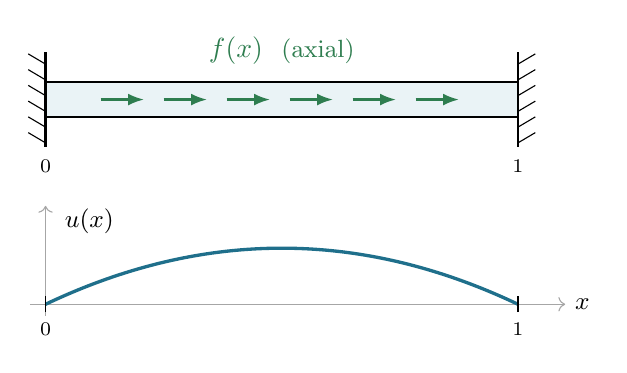
\begin{tikzpicture}[scale=1.0]
  % ---- the bar, loaded AXIALLY ----
  \draw[thick,fill=IntBack] (0,-0.22) rectangle (6,0.22);
  % supports (hatched walls)
  \draw[thick] (0,-0.6) -- (0,0.6);
  \foreach \y in {-0.55,-0.35,...,0.45} \draw (0,\y) -- (-0.22,\y+0.13);
  \draw[thick] (6,-0.6) -- (6,0.6);
  \foreach \y in {-0.55,-0.35,...,0.45} \draw (6,\y) -- (6.22,\y+0.13);
  % axial distributed load: arrows ALONG the bar
  \foreach \x in {0.7,1.5,...,5.1}
    \draw[-{Latex[length=2mm]},MEFrame,thick] (\x,0) -- (\x+0.55,0);
  \node[MEFrame] at (3.0,0.62) {$f(x)$ \ \small(axial)};
  \node at (0,-0.85) {\scriptsize$0$};
  \node at (6,-0.85) {\scriptsize$1$};
  % ---- u(x) plotted below, NOT as a sag ----
  \begin{scope}[shift={(0,-2.6)}]
    \draw[->,gray!70] (-0.2,0) -- (6.6,0) node[right,font=\small,black] {$x$};
    \draw[->,gray!70] (0,-0.15) -- (0,1.25);
    \node[right,font=\small] at (0.12,1.05) {$u(x)$};
    \draw[very thick,IntFrame] (0,0) .. controls (2,0.95) and (4,0.95) .. (6,0);
    \foreach \x/\l in {0/0, 6/1}{\draw (\x,-0.1)--(\x,0.1); \node[below,font=\scriptsize] at (\x,-0.12) {$\l$};}
  \end{scope}
\end{tikzpicture}
\end{center}

\begin{pitfall}[do not draw this as a sagging beam]
The obvious picture --- downward arrows and a drooping curve --- is
\textbf{wrong}, and the lecturer flags it directly: \emph{``misleading figure;
try to think of it as a heat transfer problem rather than a structural
mechanics problem.''}

Here $u$ is \emph{axial} displacement and $f$ is an \emph{axial} load, so the
load arrows point along the bar, and the curve below is a \emph{plot of $u$
against $x$}, not the shape the bar takes. A sagging picture silently imports
bending, which is a fourth-order problem with a different energy
($\int EI(w'')^{2}$) and different elements --- see the $H^{1}$ vs $H^{2}$
discussion later in this lecture.

The safest reading of \eqref{eq:bvp} is steady heat conduction: $u$
temperature, $a$ conductivity, $f$ a heat source. Nothing there tempts you into
bending. Use the bar for the \emph{algebra} ($au'=N$, $\int a(u')^{2}=$ strain
energy); use heat conduction for the \emph{picture}.
\end{pitfall}

\noindent
\begin{tabular}{@{}r@{\;}c@{\;}l@{\qquad}l@{}}
$u$ & $\defeq$ & ``displacement''          & \\
$f$ & $\defeq$ & ``external load''         & given\\
$a$ & $=$      & ``modulus of elasticity'' & given\\
\end{tabular}

\medskip
\noindent\textbf{Assume:}
\begin{equation}\label{eq:abounds}
  0 < a_{1} \le a(x) \le a_{2} < \infty
  \qquad \forall\, x\in[0,1].
\end{equation}

\begin{mechanics}[the model problem is an axially loaded bar]
The lecturer's own naming makes this explicit, so take it literally. Let
$a(x)=E(x)A(x)$. Then $a u'$ is the internal axial force $N(x) = EA\,\eps$, and
\eqref{eq:bvp} reads
\[
  -\frac{\dd N}{\dx} = f
  \qquad\text{i.e.}\qquad
  \frac{\dd N}{\dx} + f = 0,
\]
which is nothing but axial equilibrium of a differential slice of bar. The
boundary condition $u(0)=u(1)=0$ pins both ends.

So \eqref{eq:bvp} is: \emph{a bar, fixed at both ends, under distributed axial
load $f$, made of a material whose stiffness $a$ may vary along its length.}
Every abstract statement in the next four lectures can be checked against this
picture.

Read \eqref{eq:abounds} the same way: $a_1>0$ says the bar is nowhere made of
nothing (no zero-stiffness segment, or it would separate freely), and
$a_2<\infty$ says it is nowhere rigid. These two constants will reappear later
as the coercivity and continuity constants, and their ratio $a_2/a_1$ is the
material contrast that controls how bad the error bound gets.
\end{mechanics}

\todoq{Page 3 of my notes writes the boundary condition as $u(0)=u(1)=1$ at the
top, but every subsequent line --- and all of Lecture 2 --- uses
$u(0)=u(1)=0$. I have transcribed it as $0$. Confirm it was a slip.}

% ==================================================================
\subsection*{The operator is self-adjoint}

Note that
\begin{equation}\label{eq:Ldef}
  \mathcal{L}(u) = -(a u')'
  \qquad\text{with}\qquad u(0)=u(1)=0
\end{equation}
is a linear differential operator, and $\mathcal{L}$ is \emph{self-adjoint}.

To see it, integrate by parts twice:
\begin{align}
  \int_{0}^{1} v\,\mathcal{L}(u)\dx
    &= -\int_{0}^{1} v\,(au')'\dx \notag\\[2pt]
    &= \int_{0}^{1} v'\,a\,u'\dx - \Bigl[v\,a\,u'\Bigr]_{x=0}^{x=1}.
    \label{eq:sa1}
\end{align}
Assume $u(0)=u(1)=0$ and $v(0)=v(1)=0$; the boundary term drops:
\begin{align}
  &= \int_{0}^{1} v'\,a\,u'\dx \notag\\[2pt]
  &= -\int_{0}^{1} u\,(a v')'\dx + \Bigl[u\,a\,v'\Bigr]_{x=0}^{x=1} \notag\\[2pt]
  &= -\int_{0}^{1} u\,(a v')'\dx
   = \int_{0}^{1} u\,\mathcal{L}(v)\dx .
\end{align}

\begin{equation}\label{eq:selfadjoint}
  \boxed{\;\int_{0}^{1} v\,\mathcal{L}(u)\dx = \int_{0}^{1} u\,\mathcal{L}(v)\dx\;}
  \qquad v = \text{test function}
\end{equation}
This is what it means to be self-adjoint.

\todoq{My notes write line \eqref{eq:sa1} as
$\int v\,\mathcal{L}(u) = \int v\,(au')'$, without the minus sign, even though
$\mathcal{L}(u)=-(au')'$ two lines above. The very next line \emph{does} carry
the sign correctly, so it is a copying slip and I have restored the minus here.}

\begin{intuition}[self-adjointness is Betti's reciprocal theorem]
Equation~\eqref{eq:selfadjoint} is not a piece of abstract bookkeeping --- it is
a theorem you were taught in structures, under a different name.

Read $\mathcal{L}(u)$ as ``the load distribution that produces displacement
field $u$.'' Then the left side is \emph{the work done by load system $u$ moving
through the displacements of system $v$}, and the right side is the work done by
load system $v$ moving through the displacements of $u$. Equation
\eqref{eq:selfadjoint} says these are equal.

That is \textbf{Betti--Maxwell reciprocity}: push at $A$ and measure the
deflection at $B$; you get the same number as pushing at $B$ and measuring at
$A$. It is also exactly why the flexibility and stiffness matrices are
symmetric.
\end{intuition}

\medskip
\noindent
\textbf{Note.} A self-adjoint differential operator $\mathcal{L}$ is analogous
to a symmetric matrix.

\begin{dictionary}
$\mathcal{L}$ self-adjoint & $\Kmat = \Kmat^{T}$ \\
$\int v\,\mathcal{L}(u) = \int u\,\mathcal{L}(v)$ & $\bm{v}^{T}\Kmat\bm{u} = \bm{u}^{T}\Kmat\bm{v}$ \\
the boundary term $[v\,a\,u']_{0}^{1}$ & end reactions doing work; killed by the pinned BCs \\
$a\,u'$ & internal axial force $N = EA\,\eps$ \\
\end{dictionary}

\begin{pitfall}[the boundary term is where BCs actually enter]
Watch what happened in \eqref{eq:sa1}: the essential boundary condition was not
imposed on the equation, it was used to \emph{delete the boundary term}. This
is the mechanism for the whole subject.

Kill the term by forcing $v=0$ at the end $\Rightarrow$ that end carries an
\emph{essential} (Dirichlet, prescribed-displacement) condition, and it must be
built into the space. Kill it instead by prescribing $a u' = $ given
$\Rightarrow$ that end carries a \emph{natural} (Neumann, prescribed-traction)
condition, and it appears in the load vector for free, with nothing imposed on
the space.

That is the real content of ``essential vs.\ natural,'' and it is why in a
commercial FE code you constrain displacement DOFs explicitly but simply
\emph{apply} a traction and let the formulation absorb it.
\end{pitfall}

% ==================================================================
\subsection*{Invertibility and regularity}

\noindent\textbf{Note.} Consider
\[
  \mathcal{L}(w)=0,\qquad w(0)=w(1)=0 .
\]
The only solution that satisfies $\mathcal{L}$ and the BCs is $w=0$. Therefore
$\mathcal{L}$ is ``invertible'': for given $a$ and $f$ there exists a unique
$u$.

\begin{intuition}[trivial null space $=$ no rigid-body modes]
$\mathcal{L}(w)=0$ with $w=0$ at both ends asks: \emph{is there a nonzero
displacement field that requires no load?} For a bar pinned at both ends,
obviously not --- any nonzero shape stretches some fibre, which needs force.
Release one end and the answer changes: $w = \text{const}$ becomes a free
translation, the null space is nontrivial, and the problem has no unique
solution.

In matrix terms: $\Kmat\bm{w}=\bm{0}\Rightarrow\bm{w}=\bm{0}$ means
$\Kmat$ is nonsingular. It is the same check as ``did I constrain enough DOFs
to remove all rigid body motion,'' which is the first thing a solver complains
about when it reports a singular stiffness matrix.
\end{intuition}

\todoq{My notes read ``there exist a unique $u$ and $f$'' --- but $f$ is given
data, not something solved for. I have written ``for given $a$ and $f$ there
exists a unique $u$.'' Check the phrasing.}

\medskip
\noindent\textbf{Note (regularity).} If $0<a<\infty$ and $f$ are sufficiently
smooth --- specifically, if
\[
  a \in \Ck[(0,1)]{1}\quad\text{and}\quad f\in\Ck[(0,1)]{0},
\]
then $u\in\Ck[(0,1)]{2}$.

\begin{intuition}[the solution is two derivatives smoother than the load]
$\mathcal{L}$ takes two derivatives, so solving with $\mathcal{L}^{-1}$ gives
two back. This is the \emph{elliptic regularity} pattern, and it is why the
elliptic case is the friendly one.

It also tells you where it breaks: the hypothesis needs $a\in C^{1}$, and a bar
made of two glued materials has $a$ \emph{jumping} at the interface. Then
$u\notin C^{2}$, the strong form \eqref{eq:bvp} is not satisfied in the
classical sense, and there is no classical solution at all --- even though the
bar plainly has a displacement field. Resolving that is precisely what the
variational formulation is for, and Lecture 2 closes the loop on it.
\end{intuition}

% ==================================================================
\subsection*{Variational formulation}

Multiply our BVP by a \underline{test function} and integrate over the domain
$[0,1]$:
\begin{equation}\label{eq:mult}
  -\int_{0}^{1}(au')'\,v\dx = \int_{0}^{1} \underbrace{f}_{\text{force}} v\dx .
\end{equation}
Then integrate by parts:
\begin{equation}\label{eq:ibp1d}
  \int_{0}^{1} a\,u'v'\dx - \Bigl[a\,u'v\Bigr]_{0}^{1} = \int_{0}^{1} f v\dx .
\end{equation}
Assume $v$ satisfies the BCs:
\[
  v(0)=v(1)=0 .
\]
In particular, define the solution space
\begin{equation}\label{eq:Vdef}
  V = \left\{\, v \;:\;
    \int_{0}^{1} v^{2}\dx < \infty,\quad
    \int_{0}^{1} \bigl[v'\bigr]^{2}\dx < \infty,\quad
    v(0)=v(1)=0 \,\right\}.
\end{equation}

\begin{intuition}[$V$ is ``every shape the bar could actually take'']
Read the three conditions in \eqref{eq:Vdef} physically, in order:
\begin{itemize}[leftmargin=1.4em,itemsep=2pt]
  \item $\int v^{2}<\infty$ --- the displacement is finite in the mean. The bar
        does not fly off to infinity.
  \item $\int (v')^{2}<\infty$ --- \textbf{finite strain energy.} Since
        $v'=\eps$, this integral is (up to the factor $a/2$) the stored elastic
        energy. This is the condition that does all the work.
  \item $v(0)=v(1)=0$ --- kinematically admissible: the shape respects the
        supports.
\end{itemize}
So $V$ is the set of \emph{kinematically admissible displacement fields with
finite strain energy}. Nothing more exotic than that. This space is called
$H^{1}_{0}(0,1)$ once the course introduces Sobolev notation; when you meet that
symbol, substitute this sentence.

\medskip
\noindent\textbf{What each rung of the derivative ladder is.}
Every condition defining $V$ is a statement about one of these, and nothing in
the list goes past the first derivative:
\begin{center}\small
\renewcommand{\arraystretch}{1.15}
\begin{tabular}{@{}llll@{}}
\toprule
\textbf{Object} & \textbf{Mechanics} & \textbf{Units} & \textbf{Where it appears}\\
\midrule
$v$          & displacement            & m       & $\int v^{2}<\infty$; the BCs $v(0)=v(1)=0$\\
$v'$         & strain $\eps$           & ---     & $\int (v')^{2}<\infty$: the energy condition\\
$a v'$       & stress $\sigma$ (times area) & Pa & the flux; continuous across a material joint\\
$(a v')'$    & net force per length    & N/m     & \emph{only} in the strong form $-(av')'=f$\\
\bottomrule
\end{tabular}
\end{center}

\noindent
Because $0<a_{1}\le a\le a_{2}<\infty$, the middle two rows say the same thing:
$a_{1}^{2}\int(v')^{2}\le\int\sigma^{2}\le a_{2}^{2}\int(v')^{2}$, so ``finite
strain energy'', ``$v'$ square integrable'' and ``$\sigma$ square integrable''
are interchangeable. That two-sided bound on $a$ is exactly what keeps them
from coming apart.

\medskip
\noindent\textbf{Why $v''$ is not required.}
Two independent reasons, and it is worth holding both:
\begin{enumerate}[label=(\roman*),leftmargin=1.8em,itemsep=2pt]
  \item \textbf{The energy never contains it.} Strain energy is
        $\tfrac12\int a(v')^{2}$ --- first derivative only. A condition on
        $v''$ would be restricting something the physics does not charge for.
  \item \textbf{Integration by parts removed it.} The strong form demands
        $u''$; \eqref{eq:ibp1d} moved one derivative onto $v$, leaving $u'$ and
        $v'$. After that step $v''$ has left the problem entirely, and $u'$,
        $v'$ appear \emph{only inside integrals} --- never evaluated at a point.
\end{enumerate}

\noindent
Hence what $V$ does \emph{not} require: $v''$ need not exist, and $v'$ need not
exist in the classical sense everywhere. A hat function --- kinked, not
differentiable at its peak --- is in $V$, because that single bad point has zero
length and contributes nothing to $\int(v')^{2}$. That is deliberate: the space
was designed to be exactly big enough to hold the piecewise-linear shapes
finite elements are built from.

The whole distinction comes down to \textbf{kink versus jump}
(Figure~\ref{fig:kinkjump}), and it is worth learning once because the same two
words recur throughout the course.
\end{intuition}

% ------------------------------------------------------------------
\iftranscript\else % --- kink/jump figure: added analysis, not lecture content
\begin{figure}[htbp]
\centering
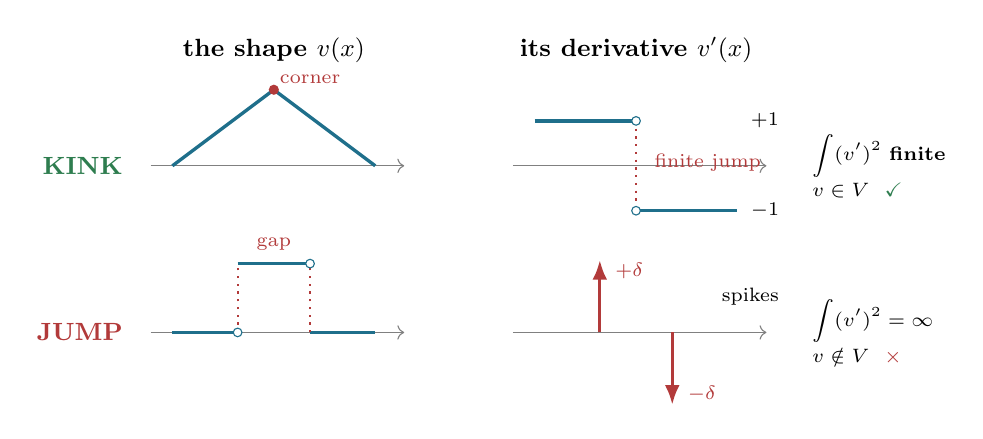
\begin{tikzpicture}[scale=0.92, every node/.style={font=\small}]

% ---------- column headers ----------
\node[font=\small\bfseries] at (1.6,3.15) {the shape $v(x)$};
\node[font=\small\bfseries] at (6.6,3.15) {its derivative $v'(x)$};

% ================= ROW 1 : KINK =================
\begin{scope}[shift={(0,1.55)}]
  \draw[->,gray] (-0.1,0) -- (3.4,0);
  \draw[very thick,IntFrame] (0.2,0) -- (1.6,1.05) -- (3.0,0);
  \fill[PitFrame] (1.6,1.05) circle (2pt);
  \node[PitFrame,above right,font=\scriptsize] at (1.55,1.0) {corner};
\end{scope}
\begin{scope}[shift={(5,1.55)}]
  \draw[->,gray] (-0.1,0) -- (3.4,0);
  \draw[very thick,IntFrame] (0.2,0.62) -- (1.6,0.62);
  \draw[very thick,IntFrame] (1.6,-0.62) -- (3.0,-0.62);
  \draw[dotted,PitFrame,thick] (1.6,0.62) -- (1.6,-0.62);
  \draw[IntFrame,fill=white] (1.6,0.62) circle (1.7pt);
  \draw[IntFrame,fill=white] (1.6,-0.62) circle (1.7pt);
  \node[right,font=\scriptsize] at (3.05,0.62) {$+1$};
  \node[right,font=\scriptsize] at (3.05,-0.62) {$-1$};
  \node[PitFrame,right,font=\scriptsize] at (1.72,0.05) {finite jump};
\end{scope}
\node[left,font=\small\bfseries,MEFrame] at (-0.35,1.55) {KINK};
\node[right,align=left,font=\scriptsize] at (8.9,1.55)
  {$\displaystyle\int (v')^{2}$ \textbf{finite}\\[1pt] $v\in V$ \ \cmark};

% ================= ROW 2 : JUMP =================
\begin{scope}[shift={(0,-0.75)}]
  \draw[->,gray] (-0.1,0) -- (3.4,0);
  \draw[very thick,IntFrame] (0.2,0) -- (1.1,0);
  \draw[very thick,IntFrame] (1.1,0.95) -- (2.1,0.95);
  \draw[very thick,IntFrame] (2.1,0) -- (3.0,0);
  \draw[dotted,PitFrame,thick] (1.1,0) -- (1.1,0.95);
  \draw[dotted,PitFrame,thick] (2.1,0) -- (2.1,0.95);
  \draw[IntFrame,fill=white] (1.1,0)    circle (1.7pt);
  \draw[IntFrame,fill=white] (2.1,0.95) circle (1.7pt);
  \node[PitFrame,above,font=\scriptsize] at (1.6,1.0) {gap};
\end{scope}
\begin{scope}[shift={(5,-0.75)}]
  \draw[->,gray] (-0.1,0) -- (3.4,0);
  \draw[very thick,-{Latex[length=2.5mm]},PitFrame] (1.1,0) -- (1.1,1.0);
  \draw[very thick,-{Latex[length=2.5mm]},PitFrame] (2.1,0) -- (2.1,-1.0);
  \node[PitFrame,right,font=\scriptsize] at (1.18,0.85) {$+\delta$};
  \node[PitFrame,right,font=\scriptsize] at (2.18,-0.85) {$-\delta$};
  \node[right,font=\scriptsize] at (2.65,0.5) {spikes};
\end{scope}
\node[left,font=\small\bfseries,PitFrame] at (-0.35,-0.75) {JUMP};
\node[right,align=left,font=\scriptsize] at (8.9,-0.75)
  {$\displaystyle\int (v')^{2}=\infty$\\[1pt] $v\notin V$ \ \xmark};

\end{tikzpicture}

\caption{\textbf{Kink versus jump.} A \emph{kink} is a break in the slope: the
shape stays connected, so the strain merely jumps between two finite values and
the energy $\int(v')^{2}$ stays finite. A \emph{jump} is a break in the shape
itself: the strain becomes a delta spike and the energy is infinite.
Mechanically, a kink is a \textbf{material interface} (steel glued to
aluminium: displacement continuous, strain jumps because $E$ jumps) --- ordinary
and everywhere. A jump is a \textbf{broken bar}. $V$ admits the first and
excludes the second, automatically, with no continuity rule written
anywhere.}
\label{fig:kinkjump}
\end{figure}
\fi

\begin{mechanics}[the same rule for beams: why they need rotational DOFs]
The rule generalises: \emph{the highest derivative appearing in the energy
fixes the space, which fixes the continuity the elements must have.} Working it
out for a beam explains an element-selection rule you already follow.

For a beam the derivative ladder is shifted up by one rung, because bending
energy lives in \emph{curvature} rather than in stretch:

\begin{center}\small
\renewcommand{\arraystretch}{1.2}
\begin{tabular}{@{}l l l@{}}
\toprule
 & \textbf{Bar (this course, for now)} & \textbf{Beam (Euler--Bernoulli)}\\
\midrule
field                & $v$ = axial displacement      & $w$ = transverse deflection\\
first derivative     & $v'$ = strain $\eps$          & $w'$ = slope $\theta$\\
second derivative    & ---                            & $w''$ = curvature $\kappa$\\
internal measure     & $\sigma = E v'$                & $M = EI\,w''$ (bending moment)\\
\textbf{energy}      & $\tfrac12\int EA\,(v')^{2}$    & $\tfrac12\int EI\,(w'')^{2}$\\
equilibrium          & $-(EA\,v')' = f$ \ (2nd order) & $(EI\,w'')'' = q$ \ (4th order)\\
space                & $H^{1}$: $\int (v')^{2}<\infty$ & $H^{2}$: $\int (w'')^{2}<\infty$\\
must stay continuous & $v$                            & $w$ \emph{and} $w'$\\
forbidden            & jump in $v$ (a break)          & jump in $w'$ (a hinge)\\
element              & $C^{0}$, DOF $\{w\}$           & $C^{1}$, DOF $\{w,\theta\}$\\
basis                & linear hat (Lagrange)          & cubic Hermite\\
\bottomrule
\end{tabular}
\end{center}

Now run the Figure~\ref{fig:kinkjump} argument one rung higher. For the bar, a
\emph{jump in $v$} gives a delta in $v'$ and infinite energy, so it is
forbidden; a \emph{kink in $v$} is fine. For the beam the energy contains
$w''$, so the thing that must not jump is $w'$:
\begin{center}
\begin{tabular}{@{}l@{\ }c@{\ }l@{\ }c@{\ }l@{}}
bar:  & jump in $v$  & $\Rightarrow$ $\delta$ in $v'$   & $\Rightarrow$ & $\int(v')^{2}=\infty$ \ \xmark\\
beam: & jump in $w'$ & $\Rightarrow$ $\delta$ in $w''$  & $\Rightarrow$ & $\int(w'')^{2}=\infty$ \ \xmark\\
\end{tabular}
\end{center}

\textbf{What a slope jump physically is: a hinge.} A kink in a beam's deflected
shape means the two sides meet at an angle. The curvature there is infinite ---
you have turned through a finite angle over zero length --- so the bending
energy $\tfrac12\int EI\kappa^{2}$ is infinite. A genuine continuous beam
cannot do this. (A real hinge \emph{can}, but only because it has $EI=0$ there,
so it stores no energy; that is a different structure, and you model it by
deliberately releasing the rotational DOF.)

\textbf{The consequence for elements.} Two adjacent bar elements sharing a node
share one number, the displacement --- and that alone makes $v$ continuous, so
$C^{0}$ suffices. Two adjacent beam elements must agree on \emph{both} the
deflection and the rotation at the shared node, or a hinge appears at every
node of your mesh. That is why a beam element carries $\{w_{1},\theta_{1},
w_{2},\theta_{2}\}$ --- four DOFs, hence a cubic ($C^{1}$ Hermite) shape
function --- while a bar element carries only $\{w_{1},w_{2}\}$.

So when a solver gives a beam or shell node rotational degrees of freedom and a
truss or solid node none, that is not a modelling convention. It is forced by
which derivative appears in the energy. Plates and shells are the 2D version of
the same statement.
\end{mechanics}

\begin{pitfall}[why the trial space suddenly needs only \emph{one} derivative]
Compare \eqref{eq:mult} with \eqref{eq:ibp1d}. Before integrating by parts, $u$
is hit with two derivatives. After, the derivatives are shared: one on $u$, one
on $v$. Nothing was approximated --- the two lines are equal --- but the
smoothness demanded of $u$ has dropped from $C^{2}$ to ``$u'$ square
integrable.''

That trade is the entire reason the weak form exists, and it is why FEM can use
$C^{0}$ elements to solve a second-order PDE. In ME language: the principle of
virtual work never asked for the second derivative of displacement in the first
place. It only ever needed strains.
\end{pitfall}

\medskip
\noindent\textbf{Note.} Functions in $V$ are continuous.
\begin{enumerate}[label=(\arabic*),leftmargin=2em,itemsep=3pt]
  \item $\displaystyle\int_{0}^{1} v^{2}\dx < \infty$ \emph{admits}
        discontinuous functions:
        \begin{center}
        \begin{tikzpicture}[scale=0.9]
          \draw[-] (-0.3,0) -- (4.3,0);
          \draw[thick] (1.0,0) -- (1.0,0.9) -- (1.8,0.9) -- (1.8,0);
          \draw (0,-0.12) -- (0,0.12);
          \draw (4,-0.12) -- (4,0.12);
          \node[below] at (0,-0.12) {\scriptsize$0$};
          \node[below] at (4,-0.12) {\scriptsize$1$};
        \end{tikzpicture}
        \end{center}
  \item $\displaystyle\int_{0}^{1}\bigl[v'\bigr]^{2}\dx$ does \emph{not} allow
        discontinuities in $V$.
\end{enumerate}

\begin{intuition}[a jump in displacement means the bar is broken]
It is condition (2), not (1), that forces continuity --- and the mechanical
reading is immediate. If $v$ jumps at a point, the bar has separated there:
a gap has opened. The strain at that point is infinite (a finite displacement
change over zero length), so the strain energy is infinite.

$V$ therefore excludes cracked configurations automatically, without anyone
writing down a continuity requirement. Requiring finite energy \emph{implies}
$C^{0}$. Lecture 2 verifies this by explicit computation with a step function,
and the answer comes out $+\infty$ exactly as this picture predicts.

This also explains the $C^{0}$ compatibility requirement you know from element
selection: adjacent elements must share displacement along their common edge,
or the assembled field has a jump there and the energy is meaningless.
\end{intuition}

% ==================================================================
\subsection*{Summary: what the strong and weak forms each demand}

\begin{pitfall}[the weak form needs $H^{1}$, \emph{not} $C^{1}$]
An easy slip is to say ``strong needs $C^{2}$, weak needs $C^{1}$.'' The second
half is wrong, and the difference is the whole point:
\begin{align*}
  C^{1}&:\ u' \text{ exists \emph{and is continuous}}
       &&\Longrightarrow\ \textbf{no kink in } u\\[2pt]
  H^{1}&:\ \textstyle\int (u')^{2}\dx<\infty,\ u' \text{ may jump}
       &&\Longrightarrow\ \textbf{kink in } u \textbf{ allowed}
\end{align*}
$H^{1}$ is \emph{weaker} than $C^{1}$:
\[
  C^{2}\ \subset\ C^{1}\ \subset\ H^{1}\ \subset\ C^{0}.
\]
Had the weak form demanded $C^{1}$, hat functions would be illegal and
piecewise-linear FEM could not exist.
\end{pitfall}

\begin{center}\small
\renewcommand{\arraystretch}{1.25}
\begin{tabular}{@{}l l l@{}}
\toprule
 & \textbf{Strong form} ($u\in\Ck[(0,1)]{2}$) & \textbf{Weak form} ($u\in V=H^{1}_{0}$)\\
\midrule
demands on $u$   & $u,u',u''$ all continuous & $u$ continuous, $\int(u')^{2}<\infty$\\
$u'$ may jump?   & no  \xmark               & \textbf{yes} \cmark\\
$u''$ required?  & yes                       & never appears\\
equation holds   & at every point            & in an integral (averaged) sense\\
\bottomrule
\end{tabular}
\end{center}

\paragraph{What the weak form buys.}
\begin{center}\small
\renewcommand{\arraystretch}{1.2}
\begin{tabular}{@{}l l l@{}}
\toprule
 & \textbf{strong} & \textbf{weak}\\
\midrule
material interface ($a$ jumps) & no solution \xmark & fine \cmark\\
point load, re-entrant corner  & no solution \xmark & fine \cmark\\
hat functions                  & illegal \xmark     & legal \cmark \ (FEM exists only here)\\
element must compute           & $u''$              & only $u'$ (the $\bm{B}$ matrix)\\
natural BC (traction)          & imposed by hand    & free --- appears in the load vector\\
existence/uniqueness           & no theory          & Lax--Milgram ($H^{1}$ is Hilbert)\\
sparsity                       & ---                & small-support kinked basis $\Rightarrow$ banded $\Kmat$\\
\bottomrule
\end{tabular}
\end{center}

\paragraph{What it costs.}
\begin{itemize}[leftmargin=1.5em,itemsep=1pt]
  \item The PDE cannot be checked at a point --- only weighted averages of it.
  \item Strain and stress come out \emph{discontinuous} across element
        boundaries; contour plots need smoothing before presentation.
  \item Derivatives are one order less accurate than the displacement, and are
        best sampled at Gauss points rather than nodes.
  \item Conceptual overhead: Sobolev spaces and weak derivatives, i.e.\ the
        first two lectures of this course.
\end{itemize}

\begin{intuition}[the trade in one line]
\[
  \textbf{strong: } \text{demand a lot of } u \;\Rightarrow\;
  \text{pointwise information, but usually \emph{no solution}}
\]
\[
  \textbf{weak: } \text{demand little of } u \;\Rightarrow\;
  \text{a solution always exists, but only in energy terms}
\]
Engineering keeps the weak form because ``no solution at all'' is a worse
problem than ``stress needs smoothing before you plot it.''
\end{intuition}

\lecture{Weak solutions: the three claims}{Lecture 2}{Math 6660 --- continues in the same OneNote export, from p.~7}

\begin{roadmap}[Lecture 2]
\roadq{Is the weak solution the same thing as the real solution?}
\begin{roadlist}
\item A weak solution is allowed to have a \textbf{kink}; a strong solution is
  not. The example: a bar whose $EA$ jumps at a point --- physically fine, but
  $u''$ does not exist there.
\item \textbf{Claim 1:} the weak solution is unique. One problem, one answer.
\item \textbf{Claim 2:} strong $\Rightarrow$ weak. Nothing is invented by going
  to the integral form.
\item \textbf{Claim 3:} weak $+$ enough smoothness $\Rightarrow$ strong. Nothing
  is lost either.
\end{roadlist}
\payoff{Trusting that the answer a virtual-work formulation produces is
\emph{the} answer, not an approximation to some neighbouring problem.}
\end{roadmap}

% ==================================================================
\subsection*{Setup, restated}

\paragraph{Two-point BVP.} On the fixed domain $0<x<1$:
\begin{equation}\label{eq:bvp2}
  -(au')' = f,
  \qquad u(0)=u(1)=0,
  \qquad \text{find } u\in\Ck[(0,1)]{2}.
\end{equation}

\paragraph{Variational formulation.}
\begin{equation}\label{eq:Vdef2}
  V = \left\{\, v \;:\;
    \int_{0}^{1} v^{2}\dx < \infty,\quad
    \int_{0}^{1} (v')^{2}\dx < \infty,\quad
    v(0)=v(1)=0 \,\right\}
  \qquad\text{(defining a space)}
\end{equation}

\noindent\textbf{Note.} Functions in $V$ are continuous
$\bigl(v\in\Ck[(0,1)]{0}\bigr)$.

\todoq{Page 7 of my notes writes the first condition as
$\int_{0}^{1}v^{2}\dx < 0$. That must be $<\infty$ --- the integrand is a
square, so $<0$ is impossible. Transcribed as $<\infty$.}

% ==================================================================
\subsection*{Example of a discontinuity}

Let
\begin{equation}\label{eq:H}
  H(x)=\begin{cases}
    1, & \tfrac14 < x < \tfrac34,\\[2pt]
    0, & \text{otherwise,}
  \end{cases}
\end{equation}
which is not continuous: $H\notin\Ck[(0,1)]{0}$, but $H\in \Ck[(0,1)]{-1}$ ---
it has a finite jump.

\begin{figure}[htbp]
\centering
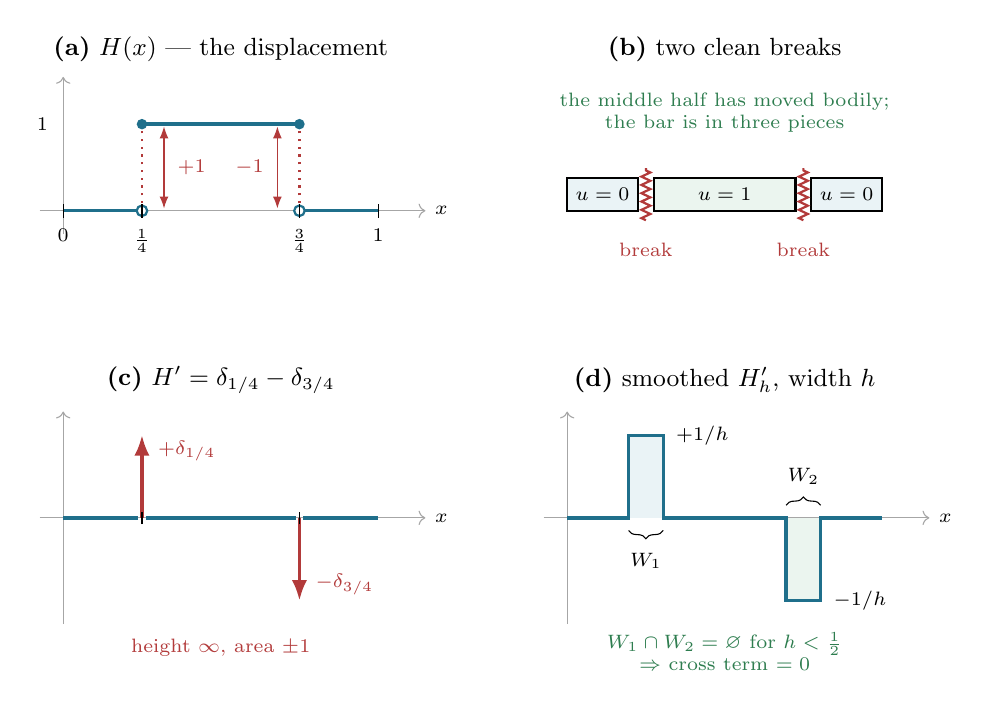
\begin{tikzpicture}[scale=1.0, every node/.style={font=\small}]

% ================= (a) H(x) =================
\begin{scope}
  \draw[->,gray!70] (-0.3,0) -- (4.6,0) node[right,font=\scriptsize,black] {$x$};
  \draw[->,gray!70] (0,-0.3) -- (0,1.7);
  \draw[very thick,IntFrame] (0,0) -- (1,0);
  \draw[very thick,IntFrame] (1,1.1) -- (3,1.1);
  \draw[very thick,IntFrame] (3,0) -- (4,0);
  \draw[dotted,thick,PitFrame] (1,0) -- (1,1.1);
  \draw[dotted,thick,PitFrame] (3,0) -- (3,1.1);
  \draw[IntFrame,fill=white,thick] (1,0)   circle (1.9pt);
  \fill[IntFrame]                  (1,1.1) circle (1.9pt);
  \fill[IntFrame]                  (3,1.1) circle (1.9pt);
  \draw[IntFrame,fill=white,thick] (3,0)   circle (1.9pt);
  \draw[{Latex[length=1.5mm]}-{Latex[length=1.5mm]},PitFrame] (1.28,0.03) -- (1.28,1.07);
  \node[PitFrame,right,font=\scriptsize] at (1.33,0.55) {$+1$};
  \draw[{Latex[length=1.5mm]}-{Latex[length=1.5mm]},PitFrame] (2.72,1.07) -- (2.72,0.03);
  \node[PitFrame,left,font=\scriptsize] at (2.67,0.55) {$-1$};
  \foreach \x/\l in {0/0, 1/{\tfrac14}, 3/{\tfrac34}, 4/1}{
    \draw (\x,-0.09) -- (\x,0.09);
    \node[below,font=\scriptsize] at (\x,-0.11) {$\l$};}
  \node[left,font=\scriptsize] at (-0.07,1.1) {$1$};
  \node[font=\small] at (2.0,2.05) {\textbf{(a)} $H(x)$ --- the displacement};
\end{scope}

% ================= (b) the bar =================
\begin{scope}[shift={(6.4,0)}]
  \fill[IntBack] (0,0) rectangle (0.9,0.42);   \draw[thick] (0,0) rectangle (0.9,0.42);
  \fill[MEBack]  (1.1,0) rectangle (2.9,0.42); \draw[thick] (1.1,0) rectangle (2.9,0.42);
  \fill[IntBack] (3.1,0) rectangle (4,0.42);   \draw[thick] (3.1,0) rectangle (4,0.42);
  \draw[decorate,decoration={zigzag,segment length=3pt,amplitude=1.6pt},PitFrame,thick]
        (1.0,-0.12) -- (1.0,0.54);
  \draw[decorate,decoration={zigzag,segment length=3pt,amplitude=1.6pt},PitFrame,thick]
        (3.0,-0.12) -- (3.0,0.54);
  \node[PitFrame,font=\scriptsize,align=center] at (1.0,-0.5) {break};
  \node[PitFrame,font=\scriptsize,align=center] at (3.0,-0.5) {break};
  \node[font=\scriptsize] at (0.45,0.21) {$u=0$};
  \node[font=\scriptsize] at (2.0,0.21)  {$u=1$};
  \node[font=\scriptsize] at (3.55,0.21) {$u=0$};
  \node[font=\small] at (2.0,2.05) {\textbf{(b)} two clean breaks};
  \node[font=\scriptsize,align=center,MEFrame] at (2.0,1.25)
       {the middle half has moved bodily;\\ the bar is in three pieces};
\end{scope}

% ================= (c) H'(x) : deltas =================
\begin{scope}[shift={(0,-3.9)}]
  \draw[->,gray!70] (-0.3,0) -- (4.6,0) node[right,font=\scriptsize,black] {$x$};
  \draw[->,gray!70] (0,-1.35) -- (0,1.35);
  \draw[very thick,IntFrame] (0,0) -- (0.95,0);
  \draw[very thick,IntFrame] (1.05,0) -- (2.95,0);
  \draw[very thick,IntFrame] (3.05,0) -- (4,0);
  \draw[very thick,-{Latex[length=2.6mm]},PitFrame] (1,0) -- (1,1.05);
  \draw[very thick,-{Latex[length=2.6mm]},PitFrame] (3,0) -- (3,-1.05);
  \node[PitFrame,right,font=\scriptsize] at (1.08,0.85)  {$+\delta_{1/4}$};
  \node[PitFrame,right,font=\scriptsize] at (3.08,-0.85) {$-\delta_{3/4}$};
  \foreach \x/\l in {1/{\tfrac14}, 3/{\tfrac34}}{
    \draw (\x,-0.08) -- (\x,0.08);}
  \node[font=\small] at (2.0,1.75) {\textbf{(c)} $H'=\delta_{1/4}-\delta_{3/4}$};
  \node[font=\scriptsize,PitFrame] at (2.0,-1.65) {height $\infty$, area $\pm1$};
\end{scope}

% ================= (d) smoothed H_h' =================
\begin{scope}[shift={(6.4,-3.9)}]
  \draw[->,gray!70] (-0.3,0) -- (4.6,0) node[right,font=\scriptsize,black] {$x$};
  \draw[->,gray!70] (0,-1.35) -- (0,1.35);
  \fill[IntBack] (0.78,0) rectangle (1.22,1.05);
  \fill[MEBack]  (2.78,0) rectangle (3.22,-1.05);
  \draw[very thick,IntFrame] (0,0) -- (0.78,0) -- (0.78,1.05) -- (1.22,1.05) -- (1.22,0)
        -- (2.78,0) -- (2.78,-1.05) -- (3.22,-1.05) -- (3.22,0) -- (4,0);
  \node[right,font=\scriptsize] at (1.26,1.05)  {$+1/h$};
  \node[right,font=\scriptsize] at (3.26,-1.05) {$-1/h$};
  \draw[decorate,decoration={brace,amplitude=3pt,mirror},thin] (0.78,-0.16) -- (1.22,-0.16);
  \node[below,font=\scriptsize] at (1.0,-0.32) {$W_{1}$};
  \draw[decorate,decoration={brace,amplitude=3pt},thin] (2.78,0.16) -- (3.22,0.16);
  \node[above,font=\scriptsize] at (3.0,0.3) {$W_{2}$};
  \node[font=\small] at (2.0,1.75) {\textbf{(d)} smoothed $H_{h}'$, width $h$};
  \node[font=\scriptsize,MEFrame,align=center] at (2.0,-1.7)
       {$W_{1}\cap W_{2}=\varnothing$ for $h<\tfrac12$\\ $\Rightarrow$ cross term $=0$};
\end{scope}

\end{tikzpicture}
\caption{The step $H$: (a) the displacement field, jumping $+1$ then $-1$;
(b) the same thing as a bar --- three pieces, two breaks; (c) its derivative,
a pair of deltas; (d) the smoothed version used for the honest calculation.}
\label{fig:step}
\end{figure}

So
\begin{equation}
  \int_{0}^{1} H^{2}\dx = \int_{1/4}^{3/4}\dx = \tfrac12 \;<\;\infty .
\end{equation}
The first condition in \eqref{eq:Vdef2} is satisfied. Now the derivative:
\begin{equation}\label{eq:Hprime}
  H'(x) = \delta\!\left(x-\tfrac14\right) - \delta\!\left(x-\tfrac34\right)
        \;=\; \delta_{1/4} - \delta_{3/4},
\end{equation}
writing $\delta_{1/4}\equiv\delta(x-\tfrac14)$ and
$\delta_{3/4}\equiv\delta(x-\tfrac34)$ --- the same objects, shorter names.
Each jump contributes one delta, sited at the jump, with coefficient equal to
the \emph{signed} jump size:
\begin{center}\small
\renewcommand{\arraystretch}{1.2}
\begin{tabular}{@{}llll@{}}
\toprule
\textbf{at} & \textbf{$H$ goes} & \textbf{size} & \textbf{contributes}\\
\midrule
$x=\tfrac14$ & $0\to1$ & $+1$ & $+\,\delta_{1/4}$\\
$x=\tfrac34$ & $1\to0$ & $-1$ & $-\,\delta_{3/4}$\\
\bottomrule
\end{tabular}
\end{center}

\begin{recall}[$\delta$ properties]
For $\delta(x-x_{0})$:
\begin{align}
  \int_{x_{0}-\eps_{1}}^{x_{0}+\eps_{2}} \delta(x-x_{0})\dx &= 1
    \qquad\text{for any }\eps_{1},\eps_{2}>0, \label{eq:delta1}\\[4pt]
  \int_{x_{0}-\eps_{1}}^{x_{0}+\eps_{2}} f(x)\,\delta(x-x_{0})\dx &= f(x_{0}),
    \qquad f \text{ a continuous function.} \label{eq:delta2}
\end{align}
\end{recall}

Now expand the square --- three terms, and \emph{all three} must be accounted
for:
\begin{align}\label{eq:Hsq}
  \int_{0}^{1}(H')^{2}\dx
    &= \int_{0}^{1}\left(\delta_{1/4}-\delta_{3/4}\right)^{2}\dx \notag\\[2pt]
    &= \int_{0}^{1}\underbrace{\delta_{1/4}^{2}}_{\text{(i)}}\dx
       \;-\;2\!\int_{0}^{1}\underbrace{\delta_{1/4}\,\delta_{3/4}}_{\text{(ii)}}\dx
       \;+\;\int_{0}^{1}\underbrace{\delta_{3/4}^{2}}_{\text{(iii)}}\dx .
\end{align}
An arrow is then drawn from term (i) down to the assertion
\begin{equation}\label{eq:sq1}
  \int_{0}^{1}\delta\!\left(x-\tfrac14\right)\delta\!\left(x-\tfrac14\right)\dx
  = +\infty ,
\end{equation}
and the conclusion $H\notin V$ follows immediately.

\todoq{Two gaps here, both in the lecture as written. \textbf{(a)} No
justification is offered for \eqref{eq:sq1} --- and \eqref{eq:delta2} cannot
supply one, since it requires $f$ to be a \emph{continuous function} while
$\delta$ is not a function at all, so $f=\delta$ is not a legal substitution.
\textbf{(b)} Only term (i) is touched; (ii) and (iii) are never addressed. The
\emph{conclusion} \eqref{eq:sq1} is correct --- the derivation below supplies
what is missing.}

% ------------------------------------------------------------------
\paragraph{The honest computation.}
Replace each jump by a ramp of width $h$. Then $H_{h}'$ is an ordinary
piecewise-constant \emph{function}:
\begin{equation}\label{eq:Hh}
  H_{h}'(x)=\begin{cases}
    +1/h, & x\in W_{1}=\left(\tfrac14-\tfrac h2,\ \tfrac14+\tfrac h2\right),\\[3pt]
    -1/h, & x\in W_{2}=\left(\tfrac34-\tfrac h2,\ \tfrac34+\tfrac h2\right),\\[3pt]
    0,    & \text{elsewhere,}
  \end{cases}
  \qquad\text{and for } h<\tfrac12,\ \ W_{1}\cap W_{2}=\varnothing .
\end{equation}
Now every term of \eqref{eq:Hsq} can be evaluated with no distributions at all:
\begin{center}\small
\renewcommand{\arraystretch}{1.35}
\begin{tabular}{@{}clll@{}}
\toprule
 & \textbf{term} & \textbf{smoothed integrand} & \textbf{integral}\\
\midrule
(i)   & $\delta_{1/4}^{2}$              & $(1/h)^{2}$ on $W_{1}$, else $0$
      & $\dfrac{1}{h^{2}}\cdot h=\dfrac1h$\\
(ii)  & $-2\,\delta_{1/4}\delta_{3/4}$  & $0$ everywhere ($W_{1}\cap W_{2}=\varnothing$)
      & $0$\\
(iii) & $\delta_{3/4}^{2}$              & $(-1/h)^{2}$ on $W_{2}$, else $0$
      & $\dfrac{1}{h^{2}}\cdot h=\dfrac1h$\\
\midrule
      & \textbf{total} & &
        $\dfrac1h+0+\dfrac1h=\dfrac{2}{h}\ \longrightarrow\ \infty$\\
\bottomrule
\end{tabular}
\end{center}

\noindent
Note (ii): the cross term vanishes for a \emph{rigorous} reason, not a
hand-wave --- the two windows are disjoint, so wherever one factor is nonzero
the other is zero. \textbf{Deltas at different places never interact.} And
(iii) contributes $+1/h$, not $-1/h$: the sign is destroyed by the square, so
the two spikes \emph{add}.

\begin{intuition}[finite area, infinite squared area]
No sampling property is needed anywhere. The one fact is
\[
  \int \delta\dx = 1 \quad\text{(finite \textbf{area})},
  \qquad\text{but}\qquad
  \int \delta^{2}\dx = \infty .
\]
A delta has finite area but \textbf{infinite height}; squaring the height beats
the shrinking width. Seen in the smoothed numbers, with $H=1/h$ and $W=h$:
\[
  \underbrace{H\cdot W = \tfrac1h\cdot h = 1}_{\text{plain: the }h\text{'s cancel}}
  \qquad\text{vs.}\qquad
  \underbrace{H^{2}\cdot W = \tfrac{1}{h^{2}}\cdot h = \tfrac1h}_{\text{squared: one }h\text{ survives below}}
\]
\end{intuition}

\begin{recall}[the plain integral passes --- as always]
Run \eqref{eq:Hh} through the \emph{unsquared} test as a control:
\[
  \int_{0}^{1}H_{h}'\dx
  = \underbrace{\left(+\tfrac1h\right)h}_{W_{1}}
  + \underbrace{\left(-\tfrac1h\right)h}_{W_{2}}
  = 1-1 = 0
  \;=\; H(1)-H(0)\quad\text{\cmark\ (FTC)} .
\]
Finite for every $h$, and independent of $h$. So the plain condition would
\emph{admit} this broken bar. Only the square rejects it.
\end{recall}

\noindent Therefore
\begin{equation}
  \boxed{\;H(x)\notin V\;}
  \qquad\text{because } H' \text{ is not square integrable.}
\end{equation}

\begin{mechanics}[the calculation behind ``the bar is broken'']
$H$ is a bar whose middle half has been translated bodily by $1$ --- two clean
breaks, at $x=\tfrac14$ and $x=\tfrac34$. Its ``strain'' $H'$ is a pair of
deltas: infinite strain at the two break points, so
$\int(H')^{2}=+\infty$ and $H$ is excluded from $V$.

Note \emph{which} test it passes and which it fails:
\begin{center}\small
\begin{tabular}{@{}lll@{}}
\toprule
test & value & verdict\\
\midrule
$\int H^{2}\dx$      & $\tfrac12$ & finite \cmark\ --- the displacement is perfectly reasonable\\
$\int H'\dx$         & $0$        & finite \cmark\ --- the plain derivative test too\\
$\int (H')^{2}\dx$   & $\infty$   & \xmark\ --- \textbf{only the energy condition rejects it}\\
\bottomrule
\end{tabular}
\end{center}
That is the precise sense in which ``finite strain energy'' is a stronger and
more physical requirement than ``bounded''.
\end{mechanics}

\begin{pitfall}[use the smoothing version in a proof]
$\delta^{2}$ is genuinely undefined --- the product of two distributions has no
meaning in general, so \eqref{eq:sq1} cannot be justified as it stands. If a
step like it appears in your own work, write the smoothed version
\eqref{eq:Hh} and take $h\to0$: same conclusion, every object an ordinary
function.
\end{pitfall}

% ==================================================================
\subsection*{The variational problem}

\begin{equation}\label{eq:varprob}
  \text{Find } u\in V \text{ such that }
  \int_{0}^{1} a\,u'v'\dx = \int_{0}^{1} f v\dx
  \qquad \text{for all } v\in V.
\end{equation}

\noindent\textbf{Note.} $u$ is the \emph{trial} function; $v$ are the
\emph{test} functions. In this case $u$ and $v$ come from the same function
space, $V$.

\begin{intuition}[this is the principle of virtual work]
Read it term by term with $a=EA$, $u'=\eps$, $v=\delta u$, $v'=\delta\eps$:
\[
  \underbrace{\int_{0}^{1} \underbrace{a u'}_{\sigma A}\;
    \underbrace{v'}_{\delta\eps}\dx}_{\text{internal virtual work}}
  \;=\;
  \underbrace{\int_{0}^{1} f\,\underbrace{v}_{\delta u}\dx}_{\text{external virtual work}}
\]
The test function is the virtual displacement. ``For all $v\in V$'' is
``for every kinematically admissible virtual displacement.'' The whole statement
is $\delta W_{\text{int}} = \delta W_{\text{ext}}$ --- equilibrium.

You have used this since undergraduate statics. What the math department adds
is not the equation but the precision about \emph{which space} $u$ and $v$ live
in, and that turns out to be the thing that makes the theory work.
\end{intuition}

\begin{pitfall}[trial $=$ test only because the BCs are homogeneous]
The note ``$u$ and $v$ come from the same function space'' is true \emph{here}
and not in general. It holds because $u(0)=u(1)=0$: the prescribed displacement
happens to be zero.

With a nonhomogeneous essential BC, say $u(0)=g\ne0$, the trial function must
satisfy $u(0)=g$ while the test function must satisfy $v(0)=0$ --- the virtual
displacement cannot violate the support. So the trial set is an affine shift of
the test space, not the same space, and it is not even a vector space. The
standard fix is to write $u = \tilde u + u_{g}$ with $\tilde u\in V$, which is
exactly what a solver does internally when it eliminates prescribed DOFs and
moves their contribution to the right-hand side.
\end{pitfall}

\medskip
\noindent\textbf{Q: How are (2-pt BVP) and (variational problem) related?}
\begin{itemize}[leftmargin=1.6em,itemsep=1pt]
  \item BVP requires $u\in\Ck[(0,1)]{2}$.
  \item Variational problem only needs $u\in V$.
\end{itemize}

\begin{intuition}[the question the next three claims answer]
Two different problems are now on the table, and they demand different amounts
of smoothness. The natural worry is whether we have quietly changed the
problem. Claims 1--3 settle it:
\begin{itemize}[leftmargin=1.4em,itemsep=2pt]
  \item \textbf{Claim 1}: the variational problem has at most one solution.
  \item \textbf{Claim 2}: every BVP solution solves the variational problem
        (the weak form is not \emph{more} restrictive).
  \item \textbf{Claim 3}: under extra smoothness, every variational solution
        solves the BVP (a partial converse).
\end{itemize}
Claim 3 needs hypotheses that Claim 2 does not. That gap is not a defect of the
proof --- it is where \emph{weak solutions} live, and the final note of the
lecture names it.
\end{intuition}

% ==================================================================
\subsection*{Claim 1: uniqueness}

\begin{proposition}
If the variational problem has a solution, it is unique.
\end{proposition}

\begin{proof}[Proof (by contradiction)]
Assume there exist 2 different solutions, $u$ and $U$:
\[
  \int_{0}^{1} a u'v'\dx = \int_{0}^{1} fv\dx
  \qquad\Big|\qquad
  \int_{0}^{1} a U'v'\dx = \int_{0}^{1} fv\dx .
\]
Then subtract:
\begin{equation}
  \Rightarrow\quad \int_{0}^{1} a\,(u-U)'\,v'\dx = 0 .
\end{equation}
Take $v = u-U \in V$. Now
\begin{equation}\label{eq:zeroenergy}
  \int_{0}^{1} a\Bigl((u-U)'\Bigr)^{2}\dx = 0
  \quad\Longrightarrow\quad (u-U)' = 0 \ \text{ on } (0,1)
  \quad\Longrightarrow\quad u = U + c .
\end{equation}
But by the BCs, $c=0$, so $u=U$.
\end{proof}

\begin{intuition}[a zero-energy difference is a rigid body motion]
Follow \eqref{eq:zeroenergy} mechanically. Suppose two different displacement
fields both equilibrate the same load. Their difference $u-U$ is then a shape
that stores \emph{zero} strain energy --- the integrand is
$a\cdot(\text{strain})^{2}$ with $a\ge a_{1}>0$, so the only way the integral
vanishes is if the strain vanishes everywhere.

Zero strain everywhere means the difference is a rigid body motion: $u-U=c$, a
uniform translation. And the supports forbid that, so $c=0$.

This is the continuum version of ``$\Kmat$ positive definite $\Rightarrow$
$\Kmat\bm{U}=\bm{F}$ has a unique solution,'' and note precisely where each
hypothesis is spent: $a\ge a_{1}>0$ gives \emph{positive} definiteness (energy
is zero only for zero strain), and the boundary conditions remove the
rigid-body null space. Drop either one and uniqueness fails --- which is exactly
what a solver tells you when it reports a singular stiffness matrix.
\end{intuition}

\begin{remark}
The lecturer labels this ``by contradiction,'' but no contradiction is actually
reached --- the argument derives $u=U$ directly. It is a direct uniqueness
proof.
\end{remark}

% ==================================================================
\subsection*{Claim 2: BVP $\Rightarrow$ variational}

\begin{proposition}
A solution to the BVP is a solution to the variational problem.
\end{proposition}

\begin{proof}
The BVP has a unique solution $u\in\Ck[(0,1)]{2}$ with $u(0)=u(1)=0$.
If $u\in\Ck[(0,1)]{2}$ and satisfies the BCs, then $u\in V$. The BVP and the
variational problem are then equivalent via integration by parts.
\end{proof}

\begin{intuition}[the easy direction, and why it is easy]
$C^{2}$ functions on a bounded interval have bounded derivatives, so
$\int (u')^{2}$ is certainly finite --- a classical solution automatically has
finite strain energy. Add the BCs and it lands in $V$. Then
\eqref{eq:mult}--\eqref{eq:ibp1d} run forward with no extra hypotheses.

The direction that costs something is the other one: going from ``the integral
identity holds for every $v$'' back to ``the differential equation holds
pointwise.'' That is Claim 3, and it needs both extra regularity \emph{and} a
genuine argument.
\end{intuition}

% ==================================================================
\subsection*{Claim 3: variational $\Rightarrow$ BVP}

\begin{proposition}\label{prop:claim3}
If $f\in\Ck[(0,1)]{0}$, $a\in\Ck[(0,1)]{1}$, and
$0<a_{1}\le a(x)\le a_{2}<\infty$ for all $x\in(0,1)$, then a solution to the
variational problem is a solution to the BVP.
\end{proposition}

\begin{proof}
Assume for the moment that $u\in\Ck[(0,1)]{2}$. From \eqref{eq:varprob},
\begin{equation}
  \int_{0}^{1}\bigl(a u'v' - fv\bigr)\dx = 0 .
\end{equation}
Reverse integration by parts:
\begin{equation}\label{eq:Sdef}
  \int_{0}^{1}\underbrace{\Bigl[(au')' + f\Bigr]}_{S(x)} v\dx = 0 .
\end{equation}

\noindent\textbf{Goal:} show $S(x)=0$ for all $x\in(0,1)$.

\medskip
\noindent\textbf{(a)} Assume, for contradiction, that
\[
  S(\xi) = \Bigl[(au')'+f\Bigr]\Big|_{x=\xi} > 0
  \qquad\text{at some point } \xi\in(0,1).
\]
Note that $S(x)$ is continuous in $x$. By continuity, $S(x)>0$ for
$x\in[\xi-\delta,\,\xi+\delta]$ for some $\delta>0$.

Choose $v$ to be the following ``hat'' function:
\begin{center}
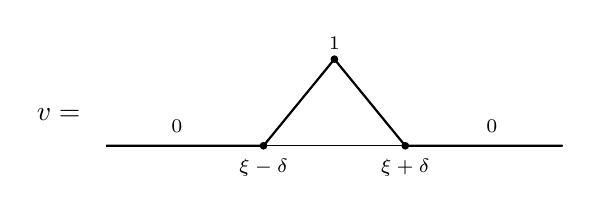
\begin{tikzpicture}[scale=1.0]
  \draw[-] (-0.4,0) -- (5.4,0);
  \draw[thick] (-0.4,0) -- (1.6,0) -- (2.5,1.1) -- (3.4,0) -- (5.4,0);
  \fill (1.6,0) circle (1.4pt);
  \fill (3.4,0) circle (1.4pt);
  \fill (2.5,1.1) circle (1.4pt);
  \node[above] at (2.5,1.1) {\scriptsize$1$};
  \node[below] at (1.6,-0.05) {\scriptsize$\xi-\delta$};
  \node[below] at (3.4,-0.05) {\scriptsize$\xi+\delta$};
  \node[above] at (0.5,0.05) {\scriptsize$0$};
  \node[above] at (4.5,0.05) {\scriptsize$0$};
  \node[left] at (-0.6,0.4) {$v=$};
\end{tikzpicture}
\end{center}
But then
\[
  \int_{0}^{1} S(x)\,v(x)\dx > 0,
\]
which is a contradiction with \eqref{eq:Sdef}. Therefore $S(x)$ cannot be
positive in $(0,1)$.

\medskip
\noindent\textbf{(b)} Redo this argument with $S(\xi)<0$
$\Rightarrow$ $S(x)$ cannot be negative in $(0,1)$.

\medskip
Hence $S\equiv0$, which is \eqref{eq:bvp2}.
\end{proof}

\begin{intuition}[the hat function is not a coincidence]
Two things are worth pausing on here.

\textbf{First, the logic.} This is the \emph{fundamental lemma of the calculus
of variations}: if $\int S v = 0$ for \emph{every} admissible $v$, then $S=0$.
The mechanical reading is the converse of virtual work --- if a leftover force
distribution $S$ does zero virtual work against every admissible virtual
displacement, there is no leftover force. The proof makes that concrete by
picking a virtual displacement that pokes the bar \emph{only} where $S$ is
claimed to be positive, so the work integral cannot cancel.

\textbf{Second, the choice of $v$.} The bump used to localise is the hat
function --- a piecewise-linear tent, one at $\xi$, zero outside
$[\xi-\delta,\xi+\delta]$. That is precisely the linear finite element basis
function $\phih_{i}$ you will build $\Vh$ from in a few lectures, and precisely
why the stiffness matrix comes out sparse (each hat overlaps only its
neighbours).

So the object introduced here as a proof device is the same object that becomes
the computational method. Worth noticing now: it is also the cleanest evidence
that $V$ was built to contain kinked functions, since a hat has no second
derivative at its peak and belongs to $V$ anyway.
\end{intuition}

\begin{pitfall}[the proof assumes what it is trying to conclude]
The proof opens with ``assume for the moment that $u\in C^{2}(0,1)$'' --- but
$u\in C^{2}$ is essentially the conclusion of Proposition~\ref{prop:claim3}.
As written, the argument shows: \emph{if} a variational solution happens to be
$C^{2}$, \emph{then} it satisfies the BVP pointwise.

Closing that gap --- proving the regularity rather than assuming it --- is a
separate theorem (elliptic regularity), and the hypotheses $f\in C^{0}$,
$a\in C^{1}$ are exactly what it needs. The lecturer's ``for the moment''
signals the debt. The final note below is where it gets paid.
\end{pitfall}

% ==================================================================
\subsection*{When can we expect $u\in\Ck[(0,1)]{2}$?}

\begin{equation}\label{eq:star}
  (\star)\qquad
  f\in\Ck[(0,1)]{0},\quad
  a\in\Ck[(0,1)]{1},\quad\text{and}\quad
  0<a_{1}\le a(x)\le a_{2}<\infty
  \quad \forall\, x\in(0,1).
\end{equation}

\noindent\textbf{Note.}
\begin{enumerate}[label=\textcircled{\scriptsize\arabic*},leftmargin=2.2em,itemsep=6pt]
  \item If $(\star)$ is satisfied: $u$ is a \emph{strong} solution of the
        2-pt BVP, and
        \[
          (\text{2-pt BVP}) \;\equiv\; (\text{variational problem}).
        \]
  \item If $(\star)$ is \emph{not} satisfied, the 2-pt BVP will not have a
        solution, but the variational problem may still have one.
        Then $u$ (if it exists) is a \emph{weak} solution of the 2-pt BVP.
\end{enumerate}

\begin{intuition}[case \textcircled{\scriptsize2} is the whole reason for the course]
This is the payoff, and it is worth stating in engineering terms because it
describes a situation you have already simulated.

Take a bar made of two materials --- steel for $x<\tfrac12$, aluminium for
$x>\tfrac12$. Then $a(x)$ \emph{jumps} at the interface, so $a\notin C^{1}$
and $(\star)$ fails. Consequently:
\begin{itemize}[leftmargin=1.4em,itemsep=2pt]
  \item The strong form has \textbf{no solution}. Not ``a hard one'' --- none.
        $u''$ does not exist at the interface, so $-(au')'=f$ is meaningless
        there.
  \item The variational problem is \textbf{completely fine}. It never asked for
        $u''$. It asks for finite strain energy, and a bimaterial bar plainly
        has that.
\end{itemize}
The physically correct answer --- displacement continuous, internal force
$au'$ continuous, strain $u'$ jumping at the interface --- is a weak solution
and not a strong one.

So the weak formulation is not a relaxation adopted for convenience. It is the
formulation under which the problem you actually want to solve \emph{has} an
answer. Every real FE model with more than one material, a contact interface, or
a point load lives in case \textcircled{\scriptsize2}.
\end{intuition}

\begin{pitfall}[``will not have a solution'' is slightly too strong]
$(\star)$ is a \emph{sufficient} condition for $u\in C^{2}$, not a necessary
one, so its failure does not by itself prove that no classical solution exists
--- one might survive by luck. The accurate statement is that the BVP
\emph{need not} have a classical solution when $(\star)$ fails, while the
variational problem still can. The bimaterial bar is a case where it genuinely
does fail.
\end{pitfall}

\begin{dictionary}[strong vs.\ weak]
strong solution & the classical one: $u\in C^{2}$, the PDE holds at every point \\
weak solution & the physical one: finite strain energy, equilibrium holds in the virtual-work sense \\
$(\star)$ fails & material interface, point load, re-entrant corner, contact \\
$u$ solves the variational problem & the structure is in equilibrium against every admissible virtual displacement \\
\end{dictionary}

\begin{intuition}[what the course has actually set up]
Standing back from Lectures 1--2, a chain has been built and it is worth
naming, because everything later hangs off it:
\[
  \underbrace{-(au')'=f}_{\text{strong form}}
  \;\longrightarrow\;
  \underbrace{\int a u'v' = \int fv \ \ \forall v\in V}_{\text{weak form}}
  \;\longrightarrow\;
  \underbrace{\text{same, with } V \text{ replaced by } \Vh}_{\text{Galerkin / FEM}}
\]
The first arrow is what these two lectures did: it costs nothing (Claims 2 and
3) and buys a problem that is solvable in realistic situations. The second arrow
has not happened yet --- it is where approximation enters, and where
$\int a u'v'$ becomes the stiffness matrix $K_{ij} = \int a\phih_{j}'\phih_{i}'$.

Keep the two arrows separate. ``Weak'' refers to the first and involves no
approximation whatsoever; the error you eventually measure comes entirely from
the second.
\end{intuition}

\lecture{Energy minimisation and the first finite element method}{Lecture 3 --- Thursday, August 27, 2026}{Math 6660 --- OneNote export \texttt{3rrd.pdf}, from p.~16}

\begin{roadmap}[Lecture 3]
\roadq{Where does ``minimum potential energy'' come from, and how does it turn
into a computer program?}
\begin{roadlist}
\item Define $F(w)=$ strain energy $-$ work done by the load. Minimising $F$
  over $\Vsp$ is \emph{exactly} the weak form --- proved, not asserted.
\item So the two derivations every FEM textbook gives, virtual work and energy
  minimisation, are one theorem stated twice.
\item Then the actual method: replace the infinite-dimensional $\Vsp$ by a
  finite-dimensional $\Vh$ of piecewise linear functions. That is
  \textbf{CG(1)}.
\item \textbf{Hat functions}: the basis in which each unknown coefficient
  \emph{is} a nodal displacement.
\end{roadlist}
\payoff{Seeing where the discretisation actually enters --- it is one step,
restricting the space, and nothing else about the problem changes.}
\end{roadmap}

% ==================================================================
\subsection*{Setup, restated}

\paragraph{2-pt BVP.}
\begin{equation}\label{eq:bvp3}
  -(au')' = f \ \text{ on } (0,1),
  \qquad u(0)=u(1)=0,
\end{equation}
with $f\in\Ck[(0,1)]{0}$, $a\in\Ck[(0,1)]{1}$, and
$0 < a_{1} \le a(x) \le a_{2} < \infty$ for all $x\in[0,1]$.

\paragraph{Variational problem.}
Find $u\in V$ such that
\begin{equation}\label{eq:var3}
  \int_{0}^{1} a\,u'v'\dx = \int_{0}^{1} f v\dx
  \qquad \forall\, v\in V,
\end{equation}
where
$V = \bigl\{ v : \int v^{2}\dx<\infty,\ \int (v')^{2}\dx<\infty,\ v(0)=v(1)=0 \bigr\}$.

\todoq{Page 16 writes the coefficient bound as $0\le a_{1} < a(x)\le a_{2}$,
but Lectures 1 and 2 both have $0 < a_{1}\le a(x)\le a_{2}$. The difference
matters: if $a_{1}=0$ were allowed, the $\eps^{2}$ coefficient in Claim
\textcircled{\scriptsize2} below could vanish and the minimiser would stop
being unique. I have used the Lecture 1 version.}

% ==================================================================
\subsection*{The ``energy'' minimisation problem}

Define the following energy functional:
\begin{equation}\label{eq:Fdef}
  F(w) \;=\;
  \underbrace{\frac12\int_{0}^{1} a\,(w')^{2}\dx}_{\text{internal energy}}
  \;-\;
  \underbrace{\int_{0}^{1} f\,w\dx}_{\text{potential energy}}
  \qquad w \text{ is a function.}
\end{equation}

\begin{mechanics}[$F$ is the total potential energy $\Pi$]
This is the most familiar object in the course so far, under a name you have
used since undergraduate structures. With $a=EA$ and $w'=\eps$:
\[
  F(w) \;=\;
  \underbrace{\tfrac12\int_{0}^{1} EA\,\eps^{2}\dx}_{\text{strain energy } U}
  \;-\;
  \underbrace{\int_{0}^{1} f\,w\dx}_{\substack{\text{work done by the applied}\\\text{load through } w}}
  \;=\; U - W \;=\; \Pi .
\]
So the Min Problem below is the \textbf{principle of minimum total potential
energy}: of all kinematically admissible displacement fields, the one that
actually occurs is the one that minimises $\Pi$. That is the principle behind
Rayleigh--Ritz, and --- as this lecture proves --- behind FEM.

Your own margin note ``not total energy'' is exactly right and worth keeping:
$F$ is the total \emph{potential} energy. There is no kinetic term because the
problem is static.
\end{mechanics}

\begin{pitfall}[``kinetic energy $-$ potential energy'' is the wrong label]
My notes annotate \eqref{eq:Fdef} with ``kinetic energy $-$ potential energy''.
That label belongs to a different principle and should not be attached here.

$L = T - V$ (kinetic minus potential) is the \emph{Lagrangian}, and the
principle that makes it stationary is Hamilton's principle, which governs
\emph{dynamics}. Equation \eqref{eq:Fdef} is static: the first term is
$\tfrac12\int EA\eps^{2}$, which is \textbf{strain energy}, not kinetic energy
--- there is no velocity anywhere in this problem.

The reason the analogy gets drawn is structural, and it is worth seeing
clearly: both functionals are ``a positive quadratic term minus a linear
term,'' and in both cases the physical state makes the functional stationary.
That shared shape is real. But the physical content of the quadratic term is
different, and conflating them will cause trouble later when the course reaches
time-dependent problems, where a genuine kinetic term $\tfrac12\int\rho\dot u^2$
appears \emph{alongside} the strain energy.
\end{pitfall}

\paragraph{Min problem.} Find $u\in V$ such that
\begin{equation}\label{eq:min}
  F(u) \le F(w) \qquad \forall\, w\in V .
\end{equation}

% ==================================================================
\subsection*{Claim: the Min Problem and the variational problem are equivalent}

\begin{theorem}\label{thm:equiv}
The minimisation problem \eqref{eq:min} and the variational problem
\eqref{eq:var3} are equivalent.
\end{theorem}

% ---------- direction 1 ----------
\paragraph{\textcircled{\scriptsize1} (variational problem) $\Rightarrow$ (Min Prob).}

Assume $u\in V$ satisfies $\int_{0}^{1}au'v'\dx = \int_{0}^{1}fv\dx$ for all
$v\in V$. Let $w\in V$, and set $w = u+v$. Then
\begin{align}
  F(w) &= F(u+v) \notag\\[2pt]
   &= \frac12\int_{0}^{1} a\,(u'+v')^{2}\dx
      - \int_{0}^{1} f u\dx - \int_{0}^{1} f v\dx \notag\\[2pt]
   &= \frac12\int_{0}^{1} a(u')^{2}\dx
    + \underbrace{\int_{0}^{1} a u'v'\dx}_{\text{(A)}}
    + \frac12\int_{0}^{1} a(v')^{2}\dx
    - \int_{0}^{1} f u\dx
    - \underbrace{\int_{0}^{1} f v\dx}_{\text{(B)}} .
    \label{eq:expand}
\end{align}
Terms (A) and (B) cancel, since (A)$\,-\,$(B)$\,=0$ is exactly the variational
problem. What remains is
\begin{equation}\label{eq:completed}
  \boxed{\;F(w) = F(u) + \frac12\int_{0}^{1} a\,(v')^{2}\dx\;}
\end{equation}
and since $a\ge a_{1}>0$, the last term is $\ge 0$. Therefore
\begin{equation}
  F(w) \;\ge\; F(u) \qquad \forall\, w\in V .
\end{equation}

\begin{intuition}[deviating from equilibrium always costs energy]
Equation \eqref{eq:completed} is the whole content of the minimum potential
energy principle, and it is worth reading slowly.

Take the true equilibrium shape $u$ and perturb it by \emph{any} admissible
amount $v$. The potential energy does not change by an amount proportional to
$v$ --- that first-order term is exactly (A)$-$(B), and it vanishes
\emph{because $u$ is in equilibrium}. What is left is a purely second-order
term, $\tfrac12\int a(v')^{2}$, which is the strain energy stored by the
perturbation itself, and it is always positive.

So: \textbf{the equilibrium configuration sits at the bottom of an energy
well.} Any wrong shape you propose stores extra strain energy and has higher
potential energy, by precisely the strain energy of your error. This is also
the algebraic ancestor of Céa's lemma and of ``FEM is too stiff'': when the
course later restricts to $\Vh$, the best you can do is the shape in $\Vh$ that
gets furthest down this well, and it can never get lower than $u$ itself.
\end{intuition}

\begin{recall}[this is just completing the square]
In finite dimensions with $\Kmat$ symmetric positive definite,
$F(\bm{w})=\tfrac12\bm{w}^{T}\Kmat\bm{w}-\bm{w}^{T}\Fvec$. Putting
$\bm{w}=\bm{u}+\bm{v}$ with $\Kmat\bm{u}=\Fvec$ gives
\[
  F(\bm{u}+\bm{v}) = F(\bm{u}) + \bm{v}^{T}(\Kmat\bm{u}-\Fvec)
                     + \tfrac12\bm{v}^{T}\Kmat\bm{v}
                   = F(\bm{u}) + \tfrac12\bm{v}^{T}\Kmat\bm{v},
\]
which is \eqref{eq:completed} term for term. Solving $\Kmat\bm{u}=\Fvec$ and
minimising $F$ are the same task --- exactly what Theorem~\ref{thm:equiv} says
in the continuous setting.
\end{recall}

\todoq{My notes conclude ``$F(w) > F(u)$'' with a strict inequality, but
\eqref{eq:completed} gives equality when $v=0$ (\ie $w=u$). It should be
$F(w)\ge F(u)$, with equality iff $w=u$. Strictness holds only for $w\ne u$.}

% ---------- direction 2 ----------
\paragraph{\textcircled{\scriptsize2} (Min Prob) $\Rightarrow$ (variational problem).}

Assume $u\in V$ satisfies $F(u)\le F(w)$ for all $w\in V$. Let
\begin{equation}
  g(\eps) = F(u+\eps v),
  \qquad\text{where } v\in V \text{ is arbitrary but fixed.}
\end{equation}
Expanding,
\begin{align}
  g(\eps) &= \frac12\int_{0}^{1} a\,(u'+\eps v')^{2}\dx
             - \int_{0}^{1} f\,(u+\eps v)\dx \notag\\[2pt]
    &= \frac12\int_{0}^{1} a(u')^{2}\dx
     + \eps\int_{0}^{1} a u'v'\dx
     + \frac12\eps^{2}\!\int_{0}^{1} a(v')^{2}\dx
     - \int_{0}^{1} f u\dx
     - \eps\int_{0}^{1} f v\dx .
\end{align}

\noindent
$g(\eps)$ is a quadratic polynomial in $\eps$ with a positive quadratic term.
The unique global minimiser happens at $\eps=0$, so $g'(0)=0$. Since
\begin{equation}\label{eq:gprime}
  g'(\eps) = \int_{0}^{1} a\,u'v'\dx - \int_{0}^{1} f v\dx
             + \eps\int_{0}^{1} a\,(v')^{2}\dx,
\end{equation}
setting $\eps=0$ gives
\begin{equation}
  g'(0) = \int_{0}^{1} a\,u'v'\dx - \int_{0}^{1} f v\dx = 0,
\end{equation}
which is exactly the variational problem. Since $v$ was arbitrary, the
variational problem is completely equivalent to this energy minimisation.
\qed

\todoq{Page 19 writes $g'(\eps)=\int u'v'\dx - \int fv\dx$, dropping the
coefficient $a$ from the first term, and the $+$ before the $\eps$ term is
missing. Both are present on the following page, so I have restored them in
\eqref{eq:gprime}.}

\begin{intuition}[$g'(0)=0$ is $\delta\Pi = 0$]
This direction is the \emph{first variation}, written out longhand. When a
mechanics text writes $\delta\Pi=0$, the operation it means is precisely
\[
  \delta\Pi = \frac{\dd}{\dd\eps}\,\Pi(u+\eps\,\delta u)\bigg|_{\eps=0} = 0 .
\]
The trick of introducing a scalar $\eps$, differentiating an ordinary
one-variable function, and setting $\eps=0$ is how a ``variation'' is made
rigorous: it converts a question about a functional on an
infinite-dimensional space into single-variable calculus along one line
through $u$.

$v$ is again the virtual displacement, and ``$v$ arbitrary but fixed'' is
``for an arbitrary admissible virtual displacement.'' So this direction says:
\emph{minimum potential energy $\Rightarrow$ virtual work}. Direction
\textcircled{\scriptsize1} said the converse. Together, they are the statement
that the energy principle and the virtual-work principle are two descriptions
of one fact.
\end{intuition}

\begin{pitfall}[the positive $\eps^{2}$ coefficient is doing real work]
Note the exact phrase: ``a quadratic polynomial in $\eps$ \emph{with a positive
quadratic term}.'' That coefficient is $\tfrac12\int a(v')^{2}$, and it is
positive only because $a\ge a_{1}>0$. It is the same coercivity assumption
that gave uniqueness in Lecture 2.

Why it matters: $g'(0)=0$ alone only makes $u$ a \emph{stationary} point.
A parabola opening upward makes it a minimum; if the quadratic coefficient
could be zero or negative, $g'(0)=0$ would still hold at a saddle or a maximum,
and \eqref{eq:min} would be false.

You have met the moment this fails. In buckling, the second variation of the
potential energy loses positive-definiteness at the critical load --- the
equilibrium is still stationary, but it stops being a minimum, and the
structure snaps to a different configuration. Everything in this course
assumes we are safely on the positive-definite side of that.
\end{pitfall}

\begin{dictionary}[the three formulations]
strong form $-(au')'=f$ & pointwise equilibrium of a differential slice \\
variational problem $\int au'v' = \int fv\ \forall v$ & principle of virtual work, $\delta W_{\text{int}}=\delta W_{\text{ext}}$ \\
min problem $F(u)\le F(w)$ & principle of minimum total potential energy \\
$g'(0)=0$ & $\delta\Pi=0$, stationary potential energy \\
$\eps^{2}$ coefficient $>0$ & $\delta^{2}\Pi>0$: the equilibrium is stable \\
\end{dictionary}

\begin{intuition}[why this equivalence is worth a whole lecture]
Three problems are now known to be the same object: the BVP (Lecture 2), the
variational problem, and the minimisation problem. That is not bookkeeping ---
each gives a different way to \emph{build} a numerical method:
\begin{itemize}[leftmargin=1.4em,itemsep=2pt]
  \item From the variational form, restrict $v$ to $\Vh$ $\Rightarrow$
        \textbf{Galerkin}.
  \item From the energy form, minimise $F$ over $\Vh$ $\Rightarrow$
        \textbf{Rayleigh--Ritz}.
\end{itemize}
For this problem --- symmetric $a$, positive definite --- the two produce the
\emph{identical} linear system. That is why the mechanics literature calls FEM
``Rayleigh--Ritz'' and the mathematics literature calls it ``Galerkin,'' and
why both are right.

The equivalence breaks when the operator is not symmetric: an advection term
$b u'$ has no energy functional to minimise, so Rayleigh--Ritz has nothing to
work with, while Galerkin still applies. That is the first hint of why the
course will keep proving things about $a(\cdot,\cdot)$ rather than about $F$.
\end{intuition}

% ==================================================================
\subsection*{Our first finite element method}

\textbf{Idea:} solve the variational problem (or the Min problem) approximately
by replacing $V$ with a finite-dimensional subspace $\Vh$.

Let $\Th$ be a mesh on $(0,1)$:
\begin{center}
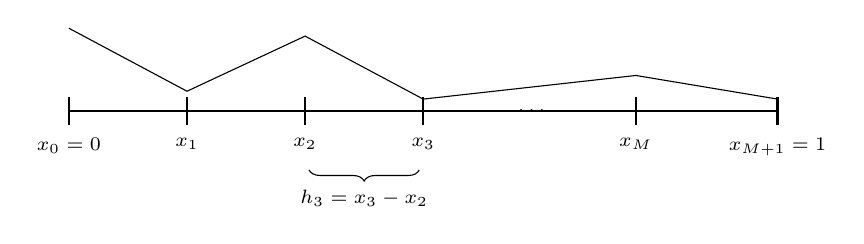
\begin{tikzpicture}[scale=1.0]
  \draw[thick] (0,0) -- (9,0);
  \foreach \x/\lab in {0/{x_{0}=0}, 1.5/{x_{1}}, 3/{x_{2}}, 4.5/{x_{3}}, 7.2/{x_{M}}, 9/{x_{M+1}=1}}{
    \draw[thick] (\x,-0.18) -- (\x,0.18);
    \node[below] at (\x,-0.22) {\scriptsize$\lab$};
  }
  \node at (5.9,0.0) {\scriptsize$\cdots$};
  % a piecewise linear function on the mesh
  \draw[thin] (0,1.05) -- (1.5,0.25) -- (3,0.95) -- (4.5,0.15) -- (7.2,0.45) -- (9,0.15);
  % brace for h_j
  \draw[decorate,decoration={brace,amplitude=4pt,mirror},thin]
        (3.05,-0.75) -- (4.45,-0.75);
  \node[below] at (3.75,-0.88) {\scriptsize$h_{3}=x_{3}-x_{2}$};
\end{tikzpicture}
\end{center}
Let
\begin{equation}
  h_{j} = x_{j} - x_{j-1},
  \qquad j = 1,2,\dots,M+1 .
\end{equation}

\medskip
The simplest $\Vh\subset V$ is the \textbf{space of continuous piecewise linear
polynomials on $\Th$}. This is called the
\begin{equation}
  \boxed{\textbf{CG(1) method}}
  \qquad
  \underbrace{\text{Continuous Galerkin method}}_{}
  \text{ with polynomials of degree } 1 .
\end{equation}

\begin{mechanics}[CG(1) is the 2-node bar element]
Strip the name and this is the element you have built by hand. ``Continuous
piecewise linear on $\Th$'' means: straight-line displacement within each
element, matching at the nodes. That is the linear 2-node bar --- constant
strain per element, and in 2D its cousin is the constant-strain triangle.

Two words carry weight:
\begin{itemize}[leftmargin=1.4em,itemsep=2pt]
  \item \textbf{Continuous}: the pieces join at the nodes. This is what makes
        $\Vh\subset V$ (``conforming''), and Lecture 2 explained why --- a jump
        would mean infinite strain energy, so a discontinuous $\Vh$ would not
        be a subspace of $V$ at all. It is your $C^{0}$ compatibility
        requirement.
  \item \textbf{(1)}: polynomial degree. CG(2) is the 3-node quadratic bar,
        and so on. Raising it is $p$-refinement; shrinking $h_{j}$ is
        $h$-refinement.
\end{itemize}
Note also that the mesh spacing $h_j$ is allowed to vary --- the elements need
not be equal length. That is local mesh refinement, available from the very
first definition.
\end{mechanics}

\medskip
Any function in $\Vh$ can be uniquely written as
\begin{equation}\label{eq:expansion}
  U(x) = \sum_{j=1}^{M} \xi_{j}\,\phih_{j}(x),
\end{equation}
where the $\xi_{j}$ are coefficients and $\phih_{j}(x)$ is the hat function
associated with $x_{j}$:
\begin{equation}\label{eq:hat}
  \phih_{j}(x) = \begin{cases}
    \dfrac{x-x_{j-1}}{h_{j}}, & x_{j-1}\le x\le x_{j},\\[10pt]
    \dfrac{x_{j+1}-x}{h_{j+1}}, & x_{j}\le x\le x_{j+1},\\[8pt]
    0, & \text{everything else, outside those limits.}
  \end{cases}
\end{equation}

\begin{center}
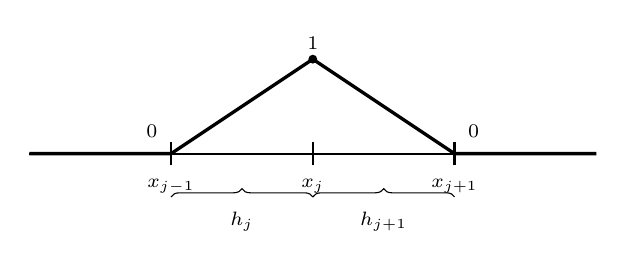
\begin{tikzpicture}[scale=1.0]
  \draw[thick] (-0.6,0) -- (6.6,0);
  \draw[very thick] (-0.6,0) -- (1.2,0) -- (3,1.2) -- (4.8,0) -- (6.6,0);
  \foreach \x/\lab in {1.2/{x_{j-1}}, 3/{x_{j}}, 4.8/{x_{j+1}}}{
    \draw[thick] (\x,-0.15) -- (\x,0.15);
    \node[below] at (\x,-0.2) {\scriptsize$\lab$};
  }
  \fill (3,1.2) circle (1.6pt);
  \node[above] at (3,1.2) {\scriptsize$1$};
  \node[left]  at (1.15,0.28) {\scriptsize$0$};
  \node[right] at (4.85,0.28) {\scriptsize$0$};
  \draw[decorate,decoration={brace,amplitude=3pt},thin] (1.2,-0.55) -- (3,-0.55);
  \node[below] at (2.1,-0.62) {\scriptsize$h_{j}$};
  \draw[decorate,decoration={brace,amplitude=3pt},thin] (3,-0.55) -- (4.8,-0.55);
  \node[below] at (3.9,-0.62) {\scriptsize$h_{j+1}$};
\end{tikzpicture}
\end{center}

\begin{intuition}[the coefficients \emph{are} the nodal displacements]
The definition \eqref{eq:hat} is engineered so that
\[
  \phih_{j}(x_{i}) = \delta_{ij}
  \qquad\text{(one at its own node, zero at every other node),}
\]
and therefore, evaluating \eqref{eq:expansion} at $x_{i}$,
\[
  U(x_{i}) = \sum_{j} \xi_{j}\,\phih_{j}(x_{i}) = \xi_{i}.
\]
So $\xi_{j}$ is not an abstract expansion coefficient --- it is
\textbf{the displacement of node $j$}. This is the property that makes FEM
usable: the unknowns you solve for are physically meaningful, boundary
conditions are imposed by setting nodal values directly, and the answer can be
plotted without post-processing. A basis without this property (a Fourier
basis, say) gives coefficients that mean nothing individually.

This is called a \emph{nodal} or \emph{Lagrange} basis, and $\xi$ is your
DOF vector $\Uvec$.
\end{intuition}

\begin{pitfall}[why the sum starts at $j=1$ and stops at $M$]
The mesh has nodes $x_{0},\dots,x_{M+1}$ --- that is $M+2$ nodes and $M+1$
elements. But \eqref{eq:expansion} sums only $j=1,\dots,M$: the
\emph{interior} nodes. The hats $\phih_{0}$ and $\phih_{M+1}$ at the two
endpoints are deliberately left out.

That omission \emph{is} the boundary condition. Every function built from
interior hats automatically satisfies $U(0)=U(1)=0$, so $\Vh\subset V$ by
construction rather than by an extra constraint. In solver terms, this is
eliminating the fixed DOFs from the system instead of penalising them, and it
is why $\dim\Vh = M$ and the stiffness matrix will be $M\times M$.

If the problem had $u(0)=g\ne0$ you would put $\phih_{0}$ back with its
coefficient \emph{fixed} at $g$ and move its column to the right-hand side ---
which is the discrete version of the trial/test distinction flagged in
Lecture 2.
\end{pitfall}

\begin{intuition}[what happens next, and why the mesh makes $\Kmat$ sparse]
The lecture stops at the definition of $\Vh$, but the next step is mechanical.
Substituting $U=\sum_{j}\xi_{j}\phih_{j}$ into \eqref{eq:var3} and testing
against each $\phih_{i}$ turns the variational problem into
\[
  \Kmat\bm{\xi}=\Fvec,
  \qquad
  K_{ij} = \int_{0}^{1} a\,\phih_{j}'\,\phih_{i}'\dx,
  \qquad
  F_{i} = \int_{0}^{1} f\,\phih_{i}\dx .
\]
Two features fall straight out of \eqref{eq:hat}:
\begin{itemize}[leftmargin=1.4em,itemsep=2pt]
  \item $\phih_{j}$ is nonzero only on $[x_{j-1},x_{j+1}]$, so
        $K_{ij}=0$ unless $\abs{i-j}\le1$: the stiffness matrix is
        \textbf{tridiagonal}. Sparsity is a consequence of choosing basis
        functions with small support, nothing more.
  \item $\phih_{j}'$ is \emph{constant} on each element ($\pm1/h$), so the
        element integrals can be done exactly by hand --- which is why the
        classical bar-element stiffness $\frac{EA}{h}\begin{psmallmatrix}1&-1\\-1&1\end{psmallmatrix}$
        looks the way it does.
\end{itemize}
\end{intuition}

\lecture{The discrete system: stiffness matrix and load vector}{Lecture 4 --- Monday, August 31, 2026}{Math 6660 --- OneNote export \texttt{4th.pdf}}

\begin{roadmap}[Lecture 4]
\roadq{How does an integral identity become $\Kmat\Uvec=\Fvec$?}
\begin{roadlist}
\item Substitute the hat basis into the weak form. The bilinear form evaluated
  on two basis functions \emph{is} the stiffness entry $K_{ij}$; the load
  functional \emph{is} $F_i$. There is nothing else in assembly.
\item \textbf{Galerkin orthogonality}: the error is orthogonal, in the energy
  inner product, to everything the mesh can represent. So the FEM answer is the
  \emph{best} member of $\Vh$, not just some member.
\item For $a\equiv1$ on a uniform mesh, $\Kmat$ comes out as the classical
  central-difference stencil --- same matrix, different reasoning.
\end{roadlist}
\payoff{Reading assembly code, and knowing why refining a mesh can never make
the energy-norm error worse.}
\end{roadmap}

% ==================================================================
\subsection*{Setup}

\paragraph{2-pt BVP.} $-(au')'=f$ on $(0,1)$, $u(0)=u(1)=0$.
\[
  \Big\Downarrow\ \text{variational problem}
\]
Find $u\in V$ such that
\begin{equation}\label{eq:var4}
  \int_{0}^{1} a\,u'v'\dx=\int_{0}^{1} f v\dx \qquad\forall\,v\in V,
\end{equation}
where $V=\bigl\{v:\int_{0}^{1}v^{2}\dx<\infty,\ \int_{0}^{1}(v')^{2}\dx<\infty,\ v(0)=v(1)=0\bigr\}$.

\paragraph{Mesh $\Th$.} Grid points
\[
  x_{0}=0,\ x_{1},\ x_{2},\ \dots,\ x_{M},\ x_{M+1}=1 .
\]

\paragraph{FEM space.}
\begin{equation}\label{eq:Vh4}
  \Vh \defeq \Bigl\{\, v\in V \;:\; v\big|_{[x_{i},x_{i+1}]}
  \in \text{polynomial of degree }1,\ \ \forall\, i=0,\dots,M \,\Bigr\}
\end{equation}

\paragraph{FEM.} Find $U\in\Vh\subset V$ such that
\begin{equation}\label{eq:fem4}
  \int_{0}^{1} a\,U'v'\dx=\int_{0}^{1} f v\dx \qquad\forall\,v\in\Vh .
\end{equation}

\begin{intuition}[the FEM problem is the variational problem with $V$ swapped for $\Vh$]
Compare the two lines: identical, except $V\to\Vh$. Nothing else changed --- not
the equation, not the bilinear form, not the load. \textbf{That single
substitution is the entire finite element method.}

This is the second arrow of Lecture 3's chain, and it is where approximation
finally enters. The first arrow (strong $\to$ weak) cost nothing.
\end{intuition}

% ==================================================================
\subsection*{A basis for $\Vh$}

$\phih_{1}(x),\phih_{2}(x),\dots,\phih_{M}(x)$, where
\begin{equation}\label{eq:hat4}
  \phih_{j}(x)=\begin{cases}
    \dfrac{x-x_{j-1}}{h_{j}}, & x_{j-1}<x<x_{j},\\[10pt]
    \dfrac{x_{j+1}-x}{h_{j+1}}, & x_{j}<x<x_{j+1},
  \end{cases}
\end{equation}
\begin{equation}
  \Vh=\operatorname{span}\{\phih_{1},\phih_{2},\dots,\phih_{M}\},
  \qquad \dim\Vh=M .
\end{equation}
If $U\in\Vh$ then
\begin{equation}\label{eq:Uexp}
  U(x)=\sum_{j=1}^{M}\xi_{j}\,\phih_{j}(x),
  \qquad\text{where}\qquad
  \xi_{j}=U(x_{j}),\quad j=1,\dots,M .
\end{equation}

\todoq{Page 2 writes the second branch of \eqref{eq:hat4} as
$(x_{j+1}-x_{j})/h_{j+1}$. That numerator is just $h_{j+1}$, so the branch would
be the constant $1$ --- not a hat. It must be $(x_{j+1}-x)/h_{j+1}$, which is
what Lecture 3 had. Transcribed corrected.}

\begin{mechanics}[$\xi_{j}$ is the displacement of node $j$]
$\xi_{j}=U(x_{j})$ is stated outright here, and it is the property that makes
the method usable: the unknowns you solve for \emph{are} the nodal
displacements, not abstract coefficients. It follows from
$\phih_{j}(x_{i})=\delta_{ij}$.

$\dim\Vh=M$ counts \emph{interior} nodes only --- $\phih_{0}$ and $\phih_{M+1}$
are absent from the basis, which is how $U(0)=U(1)=0$ is enforced. In solver
terms: the fixed DOFs were eliminated, not penalised.
\end{mechanics}

% ==================================================================
\subsection*{Galerkin orthogonality}

\begin{align}
  \int_{0}^{1}a\,u'v'\dx &= \int_{0}^{1}fv\dx, & u,v&\in V, \label{eq:go-a}\\
  \int_{0}^{1}a\,U'v'\dx &= \int_{0}^{1}fv\dx, & U,v&\in\Vh. \label{eq:go-b}
\end{align}
Subtract. Since $\Vh\subset V$, \eqref{eq:go-a} also holds for $v\in\Vh$:
\begin{equation}\label{eq:go4}
  \boxed{\;\int_{0}^{1} a\,(u-U)'\,v'\dx = 0 \qquad\text{for all } v\in\Vh\;}
\end{equation}

\begin{intuition}[the error is invisible to the mesh]
$a(\cdot,\cdot)$ is symmetric and positive definite, so it is an \emph{inner
product} --- the energy inner product. Read \eqref{eq:go4} in that language:
\[
  \bigl\langle\, u-U,\ v \,\bigr\rangle_{a} = 0 \qquad \forall\, v\in\Vh
  \qquad\Longleftrightarrow\qquad
  (u-U) \perp \Vh .
\]
So $U$ is the \textbf{orthogonal projection} of $u$ onto $\Vh$ --- the closest
point in $\Vh$ to $u$, measured in energy. Not merely a good approximation:
\emph{the best one the mesh can hold}.

Pythagoras then gives
$\Enorm{u}^{2}=\Enorm{U}^{2}+\Enorm{u-U}^{2}$, hence $\Enorm{U}\le\Enorm{u}$:
the discrete solution stores \emph{less} energy than the true one.
\textbf{A conforming displacement-based FE model is too stiff}, and refining
softens it monotonically toward the truth. That is the theorem behind the rule
of thumb.

Note where $\Vh\subset V$ was used: without it, \eqref{eq:go-a} could not be
tested against $v\in\Vh$ and the subtraction would be illegal. Conformity is
not decoration.
\end{intuition}

% ==================================================================
\subsection*{The linear system}

Put \eqref{eq:Uexp} into \eqref{eq:fem4} and take $v=\phih_{i}$,
$i=1,\dots,M$:
\begin{equation}
  \int_{0}^{1} a\Bigl(\sum_{j=1}^{M}\xi_{j}\phih_{j}\Bigr)'\phih_{i}'\dx
  = \int_{0}^{1} f\,\phih_{i}\dx
  \quad\Longrightarrow\quad
  \sum_{j=1}^{M}\xi_{j}\int_{0}^{1} a\,\phih_{i}'\phih_{j}'\dx
  = \int_{0}^{1} f\,\phih_{i}\dx .
\end{equation}
This is an $M\times M$ linear system:
\begin{equation}\label{eq:system}
  \boxed{\;\Kmat\,\bm{\xi}=\bm{b}\;}
  \qquad
  K_{ij}=\int_{0}^{1} a\,\phih_{i}'\,\phih_{j}'\dx,
  \qquad
  b_{i}=\int_{0}^{1} f\,\phih_{i}\dx,
\end{equation}
with $\bm{\xi}=(\xi_{1},\xi_{2},\dots,\xi_{M})^{T}$.

\begin{mechanics}[this is the stiffness matrix, literally]
The lecturer calls $\Kmat$ the \textbf{stiffness matrix} and lists three
properties. Each is a fact you already use:
\begin{center}\small
\renewcommand{\arraystretch}{1.25}
\begin{tabular}{@{}lll@{}}
\toprule
 & \textbf{lecture} & \textbf{you call it}\\
\midrule
(1) & symmetric: test and trial from the same space & $\Kmat=\Kmat^{T}$, Betti reciprocity\\
(2) & positive definite: $a>0$                       & no rigid-body modes; $\Kmat$ invertible\\
(3) & tridiagonal: compact support $[x_{i-1},x_{i+1}]$ & banded/sparse $\Kmat$\\
\bottomrule
\end{tabular}
\end{center}

\noindent
(1) holds because $a(u,v)=a(v,u)$ --- the same self-adjointness proved in
Lecture 1. Break it (add advection) and $\Kmat$ stops being symmetric.
(3) is purely geometric: $\phih_{i}$ lives only on $[x_{i-1},x_{i+1}]$, so
\[
  \int_{0}^{1} a\,\phih_{i}'\phih_{j}'\dx \ne 0
  \qquad\text{only for } j=i-1,\ i,\ i+1 .
\]
\end{mechanics}

\begin{figure}[htbp]
\centering
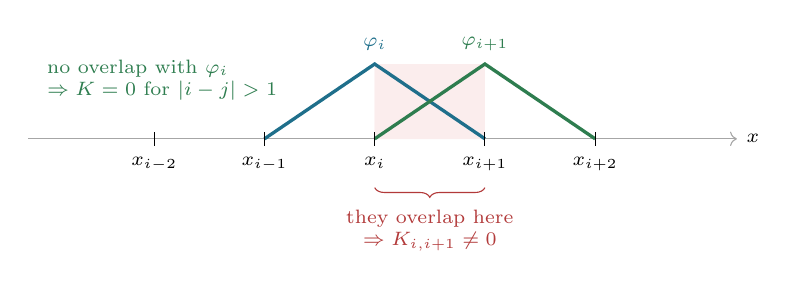
\begin{tikzpicture}[scale=1.0, every node/.style={font=\small}]
  \draw[->,gray!70] (-0.4,0) -- (8.6,0) node[right,font=\scriptsize,black] {$x$};
  % overlap shading
  \fill[PitBack] (4,0) -- (5.4,0.95) -- (5.4,0) -- cycle;
  \fill[PitBack] (4,0) -- (5.4,0.95) -- (4,0.95) -- cycle;
  \fill[PitBack] (4,0) rectangle (5.4,0.0);
  \begin{scope}
    \clip (4,0) rectangle (5.4,1.1);
    \fill[PitBack] (2.6,0) -- (4,0.95) -- (5.4,0) -- cycle;
    \fill[PitBack] (4,0) -- (5.4,0.95) -- (6.8,0) -- cycle;
  \end{scope}
  % hats
  \draw[very thick,IntFrame] (2.6,0) -- (4,0.95) -- (5.4,0);
  \draw[very thick,MEFrame]  (4,0)   -- (5.4,0.95) -- (6.8,0);
  \node[IntFrame,above,font=\scriptsize] at (4,1.0)   {$\phih_{i}$};
  \node[MEFrame,above,font=\scriptsize]  at (5.4,1.0) {$\phih_{i+1}$};
  \foreach \x/\l in {1.2/{x_{i-2}}, 2.6/{x_{i-1}}, 4/{x_{i}}, 5.4/{x_{i+1}}, 6.8/{x_{i+2}}}{
    \draw (\x,-0.09) -- (\x,0.09);
    \node[below,font=\scriptsize] at (\x,-0.11) {$\l$};}
  \draw[decorate,decoration={brace,amplitude=3.5pt,mirror},thin,PitFrame]
        (4,-0.62) -- (5.4,-0.62);
  \node[below,font=\scriptsize,PitFrame,align=center] at (4.7,-0.78)
       {they overlap here\\ $\Rightarrow K_{i,i+1}\ne0$};
  \node[font=\scriptsize,align=left,MEFrame] at (1.3,0.75)
       {no overlap with $\phih_{i}$\\ $\Rightarrow K=0$ for $\abs{i-j}>1$};
\end{tikzpicture}
\caption{Adjacent hats overlap on one element, so only $j=i-1,i,i+1$ give a
nonzero entry. Sparsity is a consequence of small support, nothing more.}
\label{fig:overlap}
\end{figure}

% ==================================================================
\subsection*{Worked example: $a\equiv1$, uniform mesh $h_{j}\equiv h$}

\paragraph{Diagonal.} $\phih_{i}'=+1/h$ on $(x_{i-1},x_{i})$ and $-1/h$ on
$(x_{i},x_{i+1})$, so $(\phih_{i}')^{2}=1/h^{2}$ on both:
\begin{align}
  K_{ii} &= \int_{0}^{1} 1\cdot\phih_{i}'\phih_{i}'\dx
        = \int_{x_{i-1}}^{x_{i}}(\phih_{i}')^{2}\dx
        + \int_{x_{i}}^{x_{i+1}}(\phih_{i}')^{2}\dx \notag\\
        &= \frac{1}{h^{2}}(x_{i}-x_{i-1}) + \frac{1}{h^{2}}(x_{i+1}-x_{i})
        = \frac{1}{h}+\frac{1}{h} = \frac{2}{h}.
\end{align}

\paragraph{Off-diagonal.} On $(x_{i},x_{i+1})$: $\phih_{i}'=-1/h$ while
$\phih_{i+1}'=+1/h$, so the product is $-1/h^{2}$ over a length $h$:
\begin{equation}
  K_{i,i+1}=\int_{x_{i}}^{x_{i+1}}\phih_{i}'\,\phih_{i+1}'\dx
  = -\frac{1}{h^{2}}\cdot h = -\frac{1}{h}.
\end{equation}

\paragraph{Load vector.} By the composite trapezoidal rule on
$[x_{i-1},x_{i+1}]$, using $\phih_{i}(x_{i\pm1})=0$ and $\phih_{i}(x_{i})=1$:
\begin{equation}
  b_{i}=\int_{x_{i-1}}^{x_{i+1}} f\,\phih_{i}\dx
  \approx \frac{h}{2}\Bigl[f(x_{i-1})\underbrace{\phih_{i}(x_{i-1})}_{0}
  + 2f(x_{i})\underbrace{\phih_{i}(x_{i})}_{1}
  + f(x_{i+1})\underbrace{\phih_{i}(x_{i+1})}_{0}\Bigr]
  = h\,f(x_{i}).
\end{equation}

\paragraph{Result.}
\begin{equation}\label{eq:tridiag}
  \Kmat=\frac{1}{h}
  \begin{bmatrix}
     2 & -1 &    &    &   \\
    -1 &  2 & -1 &    &   \\
       & -1 &  2 & -1 &   \\
       &    & \ddots & \ddots & \ddots\\
       &    &    & -1 &  2
  \end{bmatrix},
  \qquad
  \bm{b}=h\bigl(f(x_{1}),f(x_{2}),\dots,f(x_{M})\bigr)^{T}.
\end{equation}

\begin{mechanics}[this is your assembled bar stiffness]
Take the 2-node bar element of length $h$ with $EA=a=1$. Its element stiffness
is the one you derive by hand:
\[
  \bm{k}^{e}=\frac{EA}{h}\begin{bmatrix}1&-1\\-1&1\end{bmatrix}
  =\frac{1}{h}\begin{bmatrix}1&-1\\-1&1\end{bmatrix}.
\]
Assemble: node $i$ is shared by elements $(i{-}1,i)$ and $(i,i{+}1)$, so it
collects $\tfrac1h+\tfrac1h=\tfrac2h$ on the diagonal, and $-\tfrac1h$ from the
single shared element off-diagonal. That is exactly \eqref{eq:tridiag}.

\textbf{So the lecturer's $\Kmat$ and your assembled bar stiffness are the same
matrix} --- derived from a variational principle here, from equilibrium of
springs in a mechanics course. And $\bm{b}=h f(x_{i})$ is the consistent load
vector, which trapezoidal quadrature has turned into the \emph{lumped} one.
\end{mechanics}

% ==================================================================
\subsection*{Note: this is exactly the central finite difference method}

\noindent\textbf{FDM will provide the same matrix as FEM for the 2-pt BVP.} Row
$i$ of \eqref{eq:tridiag} reads
\begin{equation}
  \frac{1}{h}\bigl(-\xi_{i-1}+2\xi_{i}-\xi_{i+1}\bigr) = h\,f(x_{i})
  \qquad\Longleftrightarrow\qquad
  \frac{-\xi_{i-1}+2\xi_{i}-\xi_{i+1}}{h^{2}} = f(x_{i}),
\end{equation}
which is the $O(h^{2})$ central difference approximation of $-u''=f$.

\todoq{Page 6 reads ``FDM will also provide the same \emph{Mathematic}\dots'' ---
I think this is ``the same \emph{matrix}''. Confirm.}

\begin{pitfall}[same matrix here, different methods in general]
The two coincide only because of a stack of special choices: $a\equiv1$, a
\emph{uniform} mesh, linear elements, and trapezoidal quadrature for $\bm b$.
Change any one and they part company:
\begin{center}\small
\renewcommand{\arraystretch}{1.2}
\begin{tabular}{@{}ll@{}}
\toprule
\textbf{change} & \textbf{consequence}\\
\midrule
non-uniform $h_{j}$      & FEM handles it directly; FDM needs a new stencil\\
variable $a(x)$          & FEM integrates $a$ exactly; FDM must average it\\
exact quadrature for $\bm b$ & $\bm b\ne h f(x_{i})$ --- the systems differ\\
2D/3D, unstructured mesh & FDM has no counterpart\\
\bottomrule
\end{tabular}
\end{center}

\noindent
And they were \emph{derived} differently even here: FDM discretises the
\emph{equation}, FEM discretises the \emph{space}. That distinction --- the
first sentence of Lecture 1 --- is why FEM keeps working when the mesh stops
being a grid. Agreement on this one problem is a coincidence worth noticing,
not a general fact.
\end{pitfall}

\lecture{Nonhomogeneous Dirichlet and Neumann BCs}{Lecture 5 --- Wednesday, September 2, 2026}{Math 6660 --- \texttt{5th.pdf}}

\begin{roadmap}[Lecture 5]
\roadq{What changes when the ends are not clamped at zero?}
\begin{roadlist}
\item \textbf{Prescribed displacement} (Dirichlet, ``essential''): construct a
  function that already satisfies it and solve for the correction. This is the
  \emph{lifting} trick, and in code it is the constrained-dof step.
\item \textbf{Half-hat} basis functions appear at the boundary nodes.
\item \textbf{Prescribed force} (Neumann, ``natural''): does not constrain the
  space at all. It falls out of the integration by parts as an extra term on
  the right-hand side.
\end{roadlist}
\payoff{The essential-vs-natural distinction in one sentence: displacement BCs
modify $\Kmat$ and the space; force BCs modify $\Fvec$ only.}
\end{roadmap}

% ==================================================================
\subsection*{Nonhomogeneous Dirichlet BCs}

\begin{equation}\label{eq:nhd}
  -(au')' = f \ \text{ in } (0,1),
  \qquad u(0)=\alpha,\quad u(1)=\beta .
\end{equation}

\paragraph{Variational problem.} Integrating by parts,
\begin{equation}
  \int_{0}^{1} a u'v'\dx - \Bigl[a u'v\Bigr]_{0}^{1} = \int_{0}^{1} f v\dx .
\end{equation}
To make the boundary term vanish, define two spaces:
\begin{align}
  \Vsp   &= \Bigl\{ v : \textstyle\int_{0}^{1}\bigl[v^{2}+(v')^{2}\bigr]\dx <\infty,\ \ v(0)=\alpha,\ v(1)=\beta \Bigr\},\\
  \Vsp_0 &= \Bigl\{ v : \textstyle\int_{0}^{1}\bigl[v^{2}+(v')^{2}\bigr]\dx <\infty,\ \ v(0)=0=v(1) \Bigr\}.
\end{align}

\begin{equation}\label{eq:nhdvar}
  \text{Find } u\in \Vsp \text{ such that }
  \int_{0}^{1} a u'v'\dx = \int_{0}^{1} f v\dx
  \qquad \forall\, v\in \Vsp_{0}.
\end{equation}

\todoq{My notes write the integrability condition as $<\alpha$, but $\alpha$ is
already the boundary value. It must be $<\infty$.}

\begin{pitfall}[trial $\ne$ test --- this is the case Lecture 2 warned about]
$u\in\Vsp$ but $v\in\Vsp_{0}$. Lecture 2 noted they coincide only when the
essential BC is homogeneous; \eqref{eq:nhd} is exactly the case where they part.
$\Vsp$ is not even a vector space --- $u_1+u_2$ has boundary value $2\alpha$.
\end{pitfall}

\begin{mechanics}
$\Vsp$ = displacement fields that satisfy the prescribed support movement.
$\Vsp_{0}$ = virtual displacements, which must not violate the supports.
A settling foundation moves the structure; the virtual motion still respects it.
\end{mechanics}

% ------------------------------------------------------------------
\subsection*{Half-hat functions}

\begin{center}
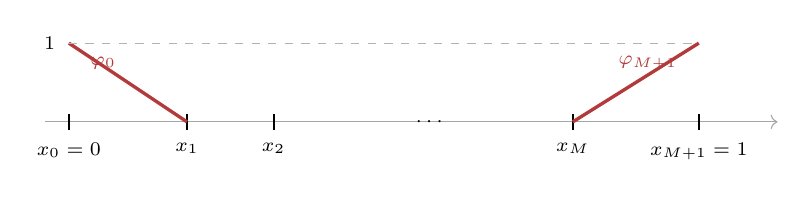
\begin{tikzpicture}[scale=1.0]
  \draw[->,gray!70] (-0.3,0) -- (9.0,0);
  \foreach \x/\l in {0/{x_{0}=0}, 1.5/{x_{1}}, 2.6/{x_{2}}, 6.4/{x_{M}}, 8.0/{x_{M+1}=1}}{
    \draw[thick] (\x,-0.1) -- (\x,0.1);
    \node[below,font=\scriptsize] at (\x,-0.14) {$\l$};}
  \node at (4.6,0) {\scriptsize$\cdots$};
  \draw[very thick,PitFrame] (0,1.0) -- (1.5,0);
  \draw[very thick,PitFrame] (6.4,0) -- (8.0,1.0);
  \draw[dashed,gray!60] (0,1.0) -- (8.0,1.0);
  \node[left,font=\scriptsize] at (-0.05,1.0) {$1$};
  \node[PitFrame,font=\scriptsize,right] at (0.15,0.75) {$\phih_{0}$};
  \node[PitFrame,font=\scriptsize,left]  at (7.85,0.75) {$\phih_{M+1}$};
\end{tikzpicture}
\end{center}

Use the same basis $\phih_{j}(x)$, $j=1,\dots,M$, and introduce two
\emph{half-hat} functions:
\begin{equation}\label{eq:halfhat}
  \phih_{0}(x)=\frac{x_{1}-x}{x_{1}-x_{0}},\ \ x\in(x_{0},x_{1});
  \qquad
  \phih_{M+1}(x)=\frac{x-x_{M}}{x_{M+1}-x_{M}},\ \ x\in[x_{M},x_{M+1}].
\end{equation}

\paragraph{Trial function.}
\begin{equation}\label{eq:lift}
  U(x) = \alpha\,\phih_{0}(x) + \beta\,\phih_{M+1}(x)
         + \sum_{j=1}^{M}\xi_{j}\,\phih_{j}(x).
\end{equation}
\paragraph{Test functions.} $v=\phih_{i}(x)$, $i=1,\dots,M$.

\medskip
\noindent
\textbf{\#} homogeneous means the boundary is zero:
$\alpha=\beta\ne0$ is \emph{not} homogeneous; $\alpha=\beta=0$ is homogeneous.

\begin{intuition}[the first two terms are a prescribed-displacement lift]
$\alpha\phih_{0}+\beta\phih_{M+1}$ is a fixed, known function that carries the
boundary data --- nothing in it is solved for. Only the $\xi_{j}$ are unknowns,
so $\dim\Vh$ is still $M$.

This is what a solver does when you prescribe a nonzero DOF: it does not add an
equation, it moves that column's contribution to the right-hand side.
\end{intuition}

% ------------------------------------------------------------------
\subsection*{The modified system}

Substituting \eqref{eq:lift} into \eqref{eq:nhdvar}:
\begin{equation}
  \sum_{j=1}^{M}\xi_{j}\int_{0}^{1} a\,\phih_{i}'\phih_{j}'\dx
  \;+\;\alpha\int_{0}^{1} a\,\phih_{0}'\phih_{i}'\dx
  \;+\;\beta\int_{0}^{1} a\,\phih_{M+1}'\phih_{i}'\dx
  \;=\;\int_{0}^{1} f\phih_{i}\dx .
\end{equation}
Moving the known terms across, and using
$\phih_{0}'=-1/h_{1}$, $\phih_{1}'=+1/h_{1}$ on $(x_{0},x_{1})$:
\begin{equation}\label{eq:nhdsystem}
  \boxed{\;
  \sum_{j=1}^{M}\xi_{j}\int_{0}^{1} a\,\phih_{i}'\phih_{j}'\dx
  = \int_{0}^{1} f\phih_{i}\dx
  + \delta_{1i}\,\frac{\alpha}{h_{1}^{2}}\int_{x_{0}}^{x_{1}} a(x)\dx
  + \delta_{Mi}\,\frac{\beta}{h_{M+1}^{2}}\int_{x_{M}}^{x_{M+1}} a(x)\dx \;}
\end{equation}

\begin{intuition}[the BC becomes a load on the first and last equation only]
The Kronecker deltas confine the new terms to rows $1$ and $M$. Every interior
equation is untouched.

Reason: $\phih_{0}$ overlaps only $\phih_{1}$, so
$\int a\,\phih_{0}'\phih_{i}'=0$ for $i\ge2$. Small support again.

Mechanically, $\Kmat$ is unchanged and $\Fvec$ picks up a reaction-like entry at
the constrained nodes --- exactly the ``move the known DOF to the RHS'' step.
\end{intuition}

\medskip
\noindent\textbf{Note.} Dirichlet BCs are enforced \emph{strongly} and modify
the RHS $\Rightarrow$ no error in the BCs. In FEM language, Dirichlet BCs are
called \textbf{essential} BCs: they must be imposed in the definition of the
function space $\Vsp$.

\todoq{My notes read ``No error in BC from BCs'' --- garbled. I have written
``no error in the BCs,'' \ie the boundary values are reproduced exactly.}

% ==================================================================
\subsection*{Neumann BCs}

\begin{equation}\label{eq:neu}
  -(au')'=f \ \text{ in } (0,1),
  \qquad
  \underbrace{u(0)=0}_{\text{Dirichlet}},
  \qquad
  \underbrace{a(1)u'(1)=g_{1}}_{\text{Neumann}} .
\end{equation}
Here
\begin{equation}\label{eq:Vneu}
  \Vsp = \Bigl\{ v : \textstyle\int_{0}^{1}\bigl(v^{2}+(v')^{2}\bigr)\dx<\infty,\ \ v(0)=0 \Bigr\}.
\end{equation}
\textbf{Only $v(0)=0$ is imposed} --- nothing is required at $x=1$.

Integrating by parts:
\begin{equation}
  \int_{0}^{1} a u'v'\dx
  - \underbrace{a(1)u'(1)}_{=\,g_{1}}v(1)
  + a(0)u'(0)\underbrace{v(0)}_{=\,0}
  = \int_{0}^{1} f v\dx ,
\end{equation}
\begin{equation}\label{eq:neuvar}
  \Longrightarrow\quad
  \int_{0}^{1} a u'v'\dx - g_{1}v(1) = \int_{0}^{1} f v\dx
  \qquad \forall\, v\in\Vsp .
\end{equation}

\begin{intuition}[the Neumann datum lands in the load vector]
Compare with the Dirichlet case. There the boundary term was \emph{killed} by
forcing $v=0$; here it is \emph{kept}, because $g_{1}$ is known. It moves to the
RHS as $+g_{1}v(1)$ --- a load, not a constraint.

$g_{1}=a(1)u'(1)=N(1)$ is the end force. So ``apply a traction'' really is just
adding a term to $\Fvec$, and that is why you constrain displacement DOFs
explicitly in a solver but merely \emph{apply} a traction.
\end{intuition}

% ------------------------------------------------------------------
\subsection*{Recovering the BVP (Neumann case)}

\textbf{Q:} is the solution of the variational problem also a solution of the
2-pt BVP?

Start from \eqref{eq:neuvar} and reverse the integration by parts:
\begin{equation}
  -\int_{0}^{1}(au')'v\dx + a(1)u'(1)v(1) = \int_{0}^{1} f v\dx + g_{1}v(1).
\end{equation}
This must hold for all $v\in\Vsp$, \emph{including} all $v\in\Vsp$ with
$v(1)=0$. For those,
\begin{equation}
  \int_{0}^{1} f v\dx = -\int_{0}^{1}(au')'v\dx
  \quad \forall\, v\in\Vsp \text{ with } v(1)=0
  \quad\Longrightarrow\quad -(au')'=f \ \text{ in } (0,1).
\end{equation}
Putting that back leaves $a(1)u'(1)v(1)=g_{1}v(1)$, and since $v(1)$ is
arbitrary,
\begin{equation}
  \boxed{\,a(1)u'(1)=g_{1}\,}
\end{equation}

\begin{intuition}[the BC was never imposed --- it fell out]
Two-stage argument: restricting to $v(1)=0$ recovers the PDE (Lecture 2's
localisation), then releasing $v(1)$ recovers the Neumann condition.

$g_{1}$ was never put into $\Vsp$, yet the solution satisfies it. That is what
\textbf{natural} means: satisfied automatically, not enforced. It is also why
Neumann data is only met approximately by the discrete solution --- see the last
note below.
\end{intuition}

% ------------------------------------------------------------------
\subsection*{CG(1) for the Neumann problem}

\begin{align}
  \Vh &= \bigl\{ v\in\Vsp : v|_{[x_{j},x_{j+1}]} = \text{polynomial of degree }1 \bigr\}\\
  \Vh &= \operatorname{span}\bigl\{\phih_{1},\phih_{2},\dots,\phih_{M},
         \underbrace{\phih_{M+1}}_{\text{new}}\bigr\}
\end{align}
$\phih_{M+1}$ is the half-hat at the right end point. Trial function:
\begin{equation}
  U(x)=\sum_{j=1}^{M+1}\xi_{j}\phih_{j}(x),
  \qquad
  \int_{0}^{1} a U'v'\dx = \int_{0}^{1} f v\dx + g_{1}v(1)
  \quad\forall\, v\in\Vh,
\end{equation}
with $v=\phih_{i}$, $i=1,2,\dots,M,\underbrace{M+1}_{\text{new}}$. Note
\begin{equation}
  \phih_{i}(1)=0 \ \ \forall\, i=1,\dots,M,
  \qquad
  \phih_{M+1}(1)=1 \ \ \text{--- the only one nonzero at } x=1 .
\end{equation}

\begin{intuition}[$M+1$ unknowns now, not $M$]
$x_{M+1}$ is no longer prescribed, so its nodal value is an unknown and the
system grows by one. Dirichlet removes a DOF; Neumann does not.

Since $\phih_{M+1}$ is the only basis function nonzero at $x=1$, the term
$g_{1}v(1)$ contributes to exactly one entry of $\Fvec$ --- the last.
\end{intuition}

\medskip
\noindent
\textbf{At $x=1$, what is the error?} $\Rightarrow$ \textbf{Not zero.}

\begin{pitfall}[Dirichlet is exact at the boundary, Neumann is not]
Strongly enforced (Dirichlet): the boundary value is built into the space, so
the discrete solution matches it \emph{exactly}. Weakly enforced (Neumann): the
condition only holds in the limit, so $a(1)U'(1)\ne g_{1}$ on a finite mesh.

You have seen this: prescribed displacements come back exactly, while reaction
forces and surface tractions carry discretisation error and need a finer mesh.
\end{pitfall}

\lecture{Neumann assembly and the first error estimate}{Lecture 6 --- Friday, September 4, 2026}{Math 6660 --- \texttt{6th.pdf}}

\begin{roadmap}[Lecture 6]
\roadq{How wrong is the FEM answer, and measured how?}
\begin{roadlist}
\item Assemble the Neumann problem explicitly first --- the boundary rows are
  where the natural BC shows up.
\item Then error analysis begins. Two \textbf{norms} matter: the energy norm
  (strain energy stored in the error) and the $L^{2}$ norm (plain size of the
  error).
\item First \textbf{a priori} estimate: the FEM error is bounded by the
  \emph{interpolation} error --- by how well the mesh could represent $u$ at
  best, regardless of the method.
\end{roadlist}
\payoff{Convergence studies: knowing what slope to expect before you run one.}
\end{roadmap}

% ==================================================================
\subsection*{Setup, restated}

\begin{equation}
  -(au')'=f \ \text{ in }(0,1),
  \qquad
  \underbrace{u(0)=0}_{\text{Dirichlet}},
  \qquad
  \underbrace{a(1)u'=g_{1}}_{\text{Neumann}}
\end{equation}
\begin{equation}
  \Vsp=\Bigl\{v:\textstyle\int\bigl[v^{2}+(v')^{2}\bigr]\dx<\infty,\ \
  \underbrace{v(0)=0}_{\text{strongly enforced}}\Bigr\}
\end{equation}

\paragraph{CG(1) method.}
\begin{equation}
  U(x)=\sum_{j=1}^{M+1}\xi_{j}\phih_{j}(x)
  \qquad
  \text{\small trial solution; the $+1$ is because the last node is unknown}
\end{equation}
\begin{equation}\label{eq:neuweak}
  \int_{0}^{1} a U'v'\dx = \int_{0}^{1} f v\dx
  + \underbrace{g_{1}v(1)}_{\text{Neumann --- weakly enforced}},
  \qquad v=\phih_{i},\ \ i=1,2,\dots,M+1 .
\end{equation}

% ==================================================================
\subsection*{Example: $a=1$, uniform mesh $h_{i}\equiv h$}

\begin{equation}
  \sum_{j=1}^{M+1}\xi_{j}\int_{0}^{1}\phih_{i}'\phih_{j}'\dx
  = \int_{0}^{1} f\phih_{i}\dx + g_{1}\phih_{i}(1)
\end{equation}

The new entries, all on the last row and column:
\begin{align}
  A_{(M,M+1)} &= \int_{x_{M}}^{x_{M+1}}\phih_{M+1}'\,\phih_{M}'\dx
    = -\frac{1}{h^{2}}\int_{x_{M}}^{x_{M+1}}\dx = -\frac{1}{h},\\
  A_{(M+1,M)} &= -\frac{1}{h}
    \qquad\Longrightarrow\quad \text{symmetric matrix},\\
  A_{(M+1,M+1)} &= \int_{x_{M}}^{x_{M+1}}\bigl(\phih_{M+1}'\bigr)^{2}\dx
    = \frac{1}{h}.
\end{align}

So $\underline{\underline{A}}\,\underline{\xi}=\underline{b}$ with
$\underline{\xi}=(\xi_{1},\xi_{2},\xi_{3},\dots,\xi_{M+1})$ and
\begin{equation}\label{eq:Aneu}
  A=\frac{1}{h}
  \begin{bmatrix}
    2 & -1 &        &    &    \\
   -1 &  2 & -1     &    &    \\
      & \ddots & \ddots & \ddots & \\
      &    & -1 & 2 & -1\\
      &    &    & -1 & \boxed{1}
  \end{bmatrix},
  \qquad
  A\in\R^{(M+1)\times(M+1)},\ \text{symmetric, positive definite.}
\end{equation}
\begin{equation}
  b_{i}=\int_{x_{i-1}}^{x_{i+1}} f\phih_{i}\dx \ \ (i=1,\dots,M),
  \qquad
  b_{M+1}=\int_{x_{M}}^{x_{M+1}} f\phih_{M+1}\dx + g_{1}.
\end{equation}

\begin{intuition}[the last diagonal entry is $1$, not $2$]
Every interior node has two elements attached, contributing $1/h$ each: hence
$2/h$. The end node $x_{M+1}$ has only \emph{one} element, so it gets $1/h$.

The $2,-1$ pattern was never a rule --- it is just ``sum of the elements meeting
at this node.'' This is exactly element-by-element assembly: each element
contributes $\frac{1}{h}\begin{psmallmatrix}1&-1\\-1&1\end{psmallmatrix}$ to its
two nodes, and the boundary node collects one copy instead of two.

Note also $g_{1}$ enters $b_{M+1}$ alone, as a plain \emph{nodal force} --- the
end traction assembled to the end node. No mystery.
\end{intuition}

\medskip
\noindent\textbf{Note: for the 2-pt BVP.}
\begin{enumerate}[label=\textcircled{\scriptsize\arabic*},leftmargin=2.2em,itemsep=2pt]
  \item Dirichlet BCs are \textbf{strongly} enforced \ (essential).
  \item Neumann or mixed BCs are \textbf{weakly} enforced \ (natural BCs).
\end{enumerate}

\begin{dictionary}[the two BC types]
essential / Dirichlet / strong & prescribed displacement; built into $\Vsp$; removes a DOF; exact\\
natural / Neumann / weak & applied traction; appears in $\Fvec$; adds no constraint; approximate\\
\end{dictionary}

% ==================================================================
\subsection*{Error analysis}

Two kinds of error estimates:
\begin{enumerate}[label=\textcircled{\scriptsize\arabic*},leftmargin=2.2em,itemsep=4pt]
  \item \textbf{a priori}: error estimate in terms of derivatives of the exact
        solution, \eg
        \[
          \underbrace{\norm{u}}_{}\;\dots\;
          \norm{\underbrace{u}_{\text{exact}}-\underbrace{U}_{\text{FEA}}}
          \;\le\; \underbrace{C}_{\text{constant}}\,
          h^{\,\underbrace{p}_{\mathclap{\text{order of shape function}}}}\,
          \norm{u^{(\ell)}}
          \qquad \ell^{\text{th}}\text{ derivative of } u .
        \]
  \item \textbf{a posteriori}: ``error estimates in terms of a residual'', \eg
        $\mathcal{L}(U)-f$. Useful for calculating error \emph{during} the
        simulation $\Rightarrow$ adaptive error control (adaptive mesh
        refinement).
\end{enumerate}

\begin{intuition}[before vs.\ after]
A priori uses $u$, which you do not have --- it predicts the \emph{rate}
($h^{p}$), so it tells you what refinement buys before you run anything.
A posteriori uses $U$, which you do have --- it says \emph{where} the error is,
which is what drives adaptive remeshing.
\end{intuition}

% ------------------------------------------------------------------
\subsection*{Norms}

Let $e(x)\defeq u(x)-U(x)$ be the error.
\begin{align}
  \text{``Energy'' norm:}  &\qquad \norm{v}_{E} = \sqrt{\int_{0}^{1} a(x)\bigl[v'(x)\bigr]^{2}\dx}\\
  \text{weighted $L_{2}$-norm:} &\qquad \norm{w}_{a} = \sqrt{\int_{0}^{1} a(x)\bigl[w(x)\bigr]^{2}\dx}
\end{align}
\begin{equation}\label{eq:normlink}
  \textbf{Note: } \norm{v}_{E}=\norm{v'}_{a}.
\end{equation}

\begin{mechanics}
$\norm{v}_{E}^{2}=\int a(v')^{2}=2\times$ strain energy. Measuring error in the
energy norm means measuring the strain energy of the error --- \ie how much
stored energy your mesh is missing. It weights \emph{strain} error, not
displacement error, which is why stress converges more slowly than displacement.
\end{mechanics}

\paragraph{Cauchy inequalities.}
\begin{align}
  \left|\int_{0}^{1} a v'w'\dx\right| &\le \norm{v'}_{a}\norm{w'}_{a}
     = \norm{v}_{E}\norm{w}_{E}, \label{eq:cauchyE}\\
  \left|\int_{0}^{1} v w\dx\right| &\le \norm{v}_{a}\norm{w}_{a^{-1}}.
\end{align}

% ------------------------------------------------------------------
\subsection*{An a priori error estimate}

CG(1) for homogeneous Dirichlet BCs: $-(au')'=f$ in $(0,1)$, $u(0)=u(1)=0$.

\paragraph{Error calculation.}
\begin{align}
  \int_{0}^{1} a U'v'\dx &= \int_{0}^{1} f v\dx \qquad \forall\, v\in\Vh\subset\Vsp, \\
  \int_{0}^{1} a u'v'\dx &= \int_{0}^{1} f v\dx \qquad \forall\, v\in\Vsp .
\end{align}
Now subtract:
\begin{equation}\label{eq:GO}
  \boxed{\;\int_{0}^{1} a\,(u-U)'\,v'\dx = 0 \qquad \forall\, v\in\Vh\;}
  \qquad \text{\textbf{Galerkin orthogonality}}
\end{equation}

\paragraph{Energy norm error estimate.} Using \eqref{eq:normlink},
\begin{equation}
  \norm{u-U}_{E}^{2} = \norm{(u-U)'}_{a}^{2}
  = \int_{0}^{1} a\,(u-U)'(u-U)'\dx .
\end{equation}
For \emph{any} $v\in\Vh$, insert $-v+v$:
\begin{align}
  \norm{u-U}_{E}^{2}
  &= \int_{0}^{1} a\,(u-U)'\,(u-v+v-U)'\dx \notag\\
  &= \int_{0}^{1} a\,(u-U)'(u-v)'\dx
   + \underbrace{\int_{0}^{1} a\,(u-U)'(v-U)'\dx}_{=\;0 \text{ by Galerkin orthogonality}} .
\end{align}

\medskip
\noindent\textbf{Note.} $u-v\in\Vsp$, but $v-U\in\Vh$ --- which is what lets
\eqref{eq:GO} kill the second term.

\begin{pitfall}[the trick is choosing which difference lies in $\Vh$]
$u-U$ is \emph{not} in $\Vh$ ($u$ is not a piecewise linear). But $v-U$
\emph{is}, since both $v$ and $U$ are. Galerkin orthogonality only annihilates
against members of $\Vh$, so the split $u-U=(u-v)+(v-U)$ is engineered to put a
$\Vh$ member in the second slot.
\end{pitfall}

\medskip
So, for any $v\in\Vh$,
\begin{equation}
  \norm{u-U}_{E}^{2} = \int_{0}^{1} a\,(u-U)'(u-v)'\dx .
\end{equation}
Using Cauchy \eqref{eq:cauchyE},
\begin{equation}
  \int_{0}^{1} a\,(u-U)'(u-v)'\dx \le \norm{(u-U)'}_{a}\,\norm{(u-v)'}_{a}
  = \norm{u-U}_{E}\,\norm{u-v}_{E},
\end{equation}
so $\norm{u-U}_{E}^{2}\le \norm{u-U}_{E}\norm{u-v}_{E}$, and cancelling one
factor:
\begin{equation}\label{eq:cea1}
  \boxed{\;\norm{u-U}_{E} \;\le\; \norm{u-v}_{E} \qquad \forall\, v\in\Vh\;}
\end{equation}
The FE solution $U$ is the best solution, meaning \emph{smallest in the energy
norm}.

\todoq{The middle line of my notes mixes the two norms
($\norm{(u-U)'}_{E}$ where it should be $\norm{u-U}_{E}$, since
$\norm{v}_{E}=\norm{v'}_{a}$ already carries the derivative). Restored above.}

\begin{intuition}[C\'ea's lemma with constant $1$]
Lecture 1's sample stated C\'ea with a factor $M/\alpha$. Here it is
\emph{exactly} $1$ --- because the energy norm is built from the same $a$ as the
bilinear form, so continuity and coercivity constants are both $1$ by
construction.

Read \eqref{eq:cea1} directly: $U$ is the closest point of $\Vh$ to $u$ in
energy. No other piecewise linear on this mesh stores a more accurate energy.
Combined with Galerkin orthogonality, $U$ is the orthogonal projection of $u$
onto $\Vh$, and Pythagoras gives $\norm{U}_{E}\le\norm{u}_{E}$ ---
\textbf{the FE model is too stiff}, as always.

Practical reading: the solver is not the limit. Accuracy is set entirely by how
well piecewise linears can represent $u$ on this mesh. Better answers come from
a better mesh, not a better solve.
\end{intuition}

\lecture{A priori error estimates: energy norm and $L^2$}{Lecture 7 --- Wednesday, September 9, 2026}{Math 6660 --- \texttt{7th.pdf}}

\begin{roadmap}[Lecture 7]
\roadq{What convergence rate, exactly?}
\begin{roadlist}
\item \textbf{Energy norm:} $O(h)$ for CG(1), and the constant is driven by
  $u''$ --- curvature of the true solution. Flat solution, small error.
\item \textbf{$L^{2}$ norm:} $O(h^{2})$, one order better. The extra order is
  not free --- it comes from a duality argument, not from the same estimate.
\item The working tool throughout is the \textbf{interpolant} $\Pi_h u$:
  compare the FEM answer to it, never directly to $u$.
\end{roadlist}
\payoff{Reading the slope on a log--log convergence plot and telling whether
your element is behaving or you have a bug.}
\end{roadmap}

% ==================================================================
\subsection*{Setup}

\begin{equation}\label{eq:l7setup}
  -(au')'=f \ \text{ in } (0,1),\qquad u(0)=u(1)=0,
\end{equation}
\begin{equation}\label{eq:l7V}
  \Vsp=\Bigl\{v:\textstyle\int_0^1\bigl[v^2+(v')^2\bigr]\dx<\infty,\ v(0)=v(1)=0\Bigr\},
  \qquad \Vh \ \text{ for CG(1)}.
\end{equation}

% ==================================================================
\subsection*{(1) Energy norm}

\begin{equation}\label{eq:l7enorm}
  \norm{e}_{E}^{2}=\int_0^1 a\bigl[(u-U)'\bigr]^{2}\dx .
\end{equation}
Last time it was shown that the FEM solution satisfies
\begin{equation}\label{eq:l7cea}
  \norm{u-U}_{E}\;\le\;\norm{u-v}_{E}
  \qquad\forall\,v\in\Vh
  \quad\text{(any other function in } \Vh).
\end{equation}

Now take the test function
\begin{equation}\label{eq:l7interp}
  v=\Pi_h u\in\Vh,
  \qquad
  \Pi_h u=\sum_{j=1}^{M} u(x_j)\,\phih_j(x),
\end{equation}
the projection of $u\in\Vsp$ into the subspace $\Vh\subset\Vsp$: interpolate
$u(x)$ onto the mesh using piecewise linear (continuous) functions.

\todoq{Page 2 writes the sum as $\sum_{j=1}^{M}u(x_i)\phih_i(x)$ --- the index
under the sum is $j$ but the terms carry $i$. Transcribed with $j$ throughout.
The word before ``functions'' is hard to read; from context it must be
\emph{linear}, not \emph{Green}.}

\begin{intuition}[what $\Pi_h u$ is, and why it is the right test function]
$\Pi_h u$ is the piecewise-linear function that \emph{agrees with $u$ at every
node} --- connect the dots of the exact solution with straight lines. It is
computable in principle and, crucially, it is a legal member of $\Vh$.

Why feed it into \eqref{eq:l7cea}: that inequality holds for \emph{every}
$v\in\Vh$, so it holds for the one we can estimate. C\'ea says $U$ is at least
as good as $\Pi_h u$, so bounding how badly a straight line approximates $u$ on
one element bounds the entire FE error. The solver never enters.
\end{intuition}

\medskip\noindent\textbf{Note.}
\begin{equation}\label{eq:l7interperr}
  \norm{u-\Pi_h u}_{E}=\norm{(u-\Pi_h u)'}_{a}\le C\,\norm{h\,u''}_{a},
\end{equation}
which just comes from approximating $u'$ by a piecewise constant function; $C$
is a constant that depends only on $a(x)$.

\begin{theorem}\label{thm:l7apriori}
The FEM approximation $U\in\Vh$ satisfies $\norm{u-U}_{E}\le\norm{u-v}_{E}$ for
all $v\in\Vh\subset\Vsp$. In particular there exists a constant $C$, depending
only on $a(x)$, such that
\begin{equation}\label{eq:l7thm}
  \boxed{\ \norm{u-U}_{E}\le C\,\norm{h\,u''}_{a}\ }
\end{equation}
\end{theorem}

\medskip\noindent\textbf{Note.} This shows that CG(1) is \emph{first order
accurate in the energy norm}, provided $u''\in L^{2}(0,1)$.

\begin{mechanics}[what first order buys you]
Halve the mesh, halve the energy-norm error. And the energy norm weights
\emph{strain}, so \eqref{eq:l7thm} is a statement about stress accuracy.

Note the proviso: $u''\in L^{2}$. At a re-entrant corner or a point load $u''$
is not square integrable, the right-hand side is infinite, and the estimate
says nothing --- which is exactly the case where uniform refinement stalls.
\end{mechanics}

% ==================================================================
\subsection*{(2) $L^{2}(0,1)$ norm}

For the same problem \eqref{eq:l7setup}, consider the following
\textbf{dual problem}:
\begin{equation}\label{eq:l7dual}
  -(a\phi')'=e,\qquad \phi(0)=\phi(1)=0,
  \qquad\text{where } e=u-U .
\end{equation}

\medskip\noindent\textbf{Note.} Because the original 2-pt BVP is self-adjoint,
the primal and dual operators are the same.

\begin{intuition}[the dual problem, and why self-adjointness matters]
The dual problem is an auxiliary BVP whose \emph{load is the error itself}.
Solve it and you obtain a $\phi$ engineered so that pairing it against $e$
reproduces $\norm{e}^{2}$ --- which is the whole trick below.

Self-adjointness (Lecture 1's Green's formula) is what makes the dual operator
identical to the primal one. For a non-self-adjoint problem you would have to
solve a genuinely different equation here.
\end{intuition}

\paragraph{$L^{2}$-norm.} Multiply \eqref{eq:l7dual} by $e$ and integrate:
\begin{align}
  \norm{e}^{2}
   &= \int_0^1 e^{2}\dx
    = -\int_0^1 e\,(a\phi')'\dx \notag\\
   &= \int_0^1 a\,e'\phi'\dx - \Bigl[a\,e\,\phi'\Bigr]_0^1 ,
   \label{eq:l7ibp}
\end{align}
and the boundary term vanishes because $e(0)=e(1)=0$, so
\begin{equation}\label{eq:l7esq}
  \norm{e}^{2}=\int_0^1 a\,e'\phi'\dx .
\end{equation}

\medskip\noindent
\textbf{Recall Galerkin orthogonality:}
$\int_0^1 a\,e'v'\dx=0$ for all $v\in\Vh$. Take $v=\Pi_h\phi$:
\begin{equation}\label{eq:l7GO}
  \norm{e}^{2}
   = \int_0^1 a\,e'\phi'\dx-\int_0^1 a\,e'\,(\Pi_h\phi)'\dx
   = \int_0^1 a\,e'\,(\phi-\Pi_h\phi)'\dx .
\end{equation}

\begin{intuition}[subtracting zero is the whole move]
$\int a\,e'(\Pi_h\phi)'\dx$ is zero by Galerkin orthogonality, so
\eqref{eq:l7GO} subtracts nothing. But it converts $\phi'$ into the
\emph{interpolation error} $(\phi-\Pi_h\phi)'$, which is small --- order $h$ ---
whereas $\phi'$ itself is not small at all. That single substitution is what
buys the extra power of $h$.
\end{intuition}

\paragraph{Cauchy's inequality.}
\begin{align}
  \norm{e}^{2} &\le \norm{e'}_{a}\,\norm{(\phi-\Pi_h\phi)'}_{a}
   \label{eq:l7cauchy}\\
  \norm{e}^{2} &\le C_{I}\,h_{\max}\,\norm{e'}_{a}\,
                    \underbrace{\norm{\phi''}_{a}}_{\text{interpolation error}}
   \label{eq:l7cauchy2}
\end{align}
But recall, from part (1),
\begin{equation}\label{eq:l7recall}
  \norm{e'}_{a}=\norm{e}_{E}\le C_{I}\,h_{\max}\,\norm{u''}_{a},
\end{equation}
so
\begin{equation}\label{eq:l7chain}
  \norm{e}^{2}\le C_{I}^{2}\,h_{\max}^{2}\,\norm{u''}_{a}\,\norm{\phi''}_{a}
  = C_{I}^{2}\,h_{\max}^{2}\,\norm{u''}_{a}\,
    \frac{\norm{\phi''}_{a}}{\norm{e}}\,\norm{e},
\end{equation}
and dividing by $\norm{e}$,
\begin{equation}\label{eq:l7L2}
  \norm{e}\le C_{I}^{2}\,h_{\max}^{2}\,\norm{u''}_{a}\,
              \frac{\norm{\phi''}_{a}}{\norm{e}} .
\end{equation}
Let
\begin{equation}\label{eq:l7Sa}
  S_{a}=\max_{\xi\neq0}\frac{\norm{\psi''}_{a}}{\norm{\xi}},
  \qquad\text{where}\qquad
  -(a\psi')'=\xi,\quad \psi(0)=\psi(1)=0 .
\end{equation}

\medskip\noindent\textbf{Note.} If $a\equiv$ constant, then
$-(a\psi')'=-a\psi''=\xi$, so
\begin{equation}\label{eq:l7const}
  \frac{\psi''}{\norm{\xi}}=\frac{1}{a}.
\end{equation}

\todoq{Two things to check here. (i) The last line divides a \emph{function}
$\psi''$ by a \emph{number} $\norm{\xi}$; it should presumably read
$\norm{\psi''}/\norm{\xi}=1/a$, and the sign from $\psi''=-\xi/a$ has been
dropped. (ii) That $1/a$ comes out only if the numerator is the plain $L^2$
norm, not the $a$-weighted $\norm{\cdot}_a$ used in \eqref{eq:l7Sa} --- with the
weighted norm one gets $1/\sqrt{a}$. Ask which norm is meant in $S_a$.}

\begin{intuition}[the payoff: $L^2$ converges one order faster]
Combining \eqref{eq:l7L2} with \eqref{eq:l7Sa} gives
$\norm{e}\le C_{I}^{2}h_{\max}^{2}S_{a}\norm{u''}_{a}$ --- \textbf{second}
order in $h$, against first order for the energy norm \eqref{eq:l7thm}.

Where the extra power came from: interpolation error was used \emph{twice} ---
once on $e$ through \eqref{eq:l7recall}, once on $\phi$ through
\eqref{eq:l7GO}. Each contributes one factor of $h$. This is the duality
(Aubin--Nitsche) argument.

Engineering reading: \textbf{displacements converge faster than stresses}. The
energy norm measures strain error and gives $O(h)$; the $L^2$ norm measures
displacement error and gives $O(h^2)$. That is why a displacement plot can look
converged while the stress plot is still visibly wrong.
\end{intuition}

\todoq{The notes stop at \eqref{eq:l7const} without writing the final $L^2$
estimate explicitly. Confirm the intended statement is
$\norm{e}\le C_I^{2}h_{\max}^{2}S_a\norm{u''}_a$.}

\lecture{The stability constant, and a posteriori error}{Lecture 8 --- Friday, September 11, 2026}{Math 6660 --- \texttt{8th.pdf}}

\begin{roadmap}[Lecture 8]
\roadq{Why does the $L^{2}$ estimate get an extra power of $h$, and what is the
difference between the two kinds of error bound?}
\begin{roadlist}
\item The duality argument needs a \textbf{stability constant} $C_{S}$: the
  auxiliary (dual) problem's solution must not blow up. That is what is proved
  here.
\item The \textbf{Poincar\'e inequality} is the tool that delivers it --- a
  function pinned at the boundary cannot be large if its derivative is small.
\item Result: $\norm{e}\le C\,h^{2}\norm{u''}$.
\item Then the switch: \textbf{a priori} bounds involve $u$, which you do not
  have. \textbf{A posteriori} bounds involve $U$, which you just computed.
\end{roadlist}
\payoff{Separating ``what rate should this element give'' from ``how wrong is
\emph{this particular} run''.}
\end{roadmap}

% ==================================================================
\subsection*{Recap}

For $-(au')'=f$ on $(0,1)$, $u(0)=u(1)=0$, with CG(1):

\paragraph{(1) Energy norm.}
$\norm{u-U}_{E}^{2}=\int_0^1 a\bigl[(u-U)'\bigr]^{2}\dx$, and
$\norm{u-U}_{E}\le\norm{u-v}_{E}$ for all $v\in\Vh$. Taking $v=\Pi_h u$,
\begin{equation}\label{eq:l8e}
  \norm{e}_{E}\le C\,\norm{h\,u''}_{a}.
\end{equation}

\paragraph{(2) $L^{2}$ norm.}
$\norm{u-U}^{2}=\int_0^1 (u-U)^{2}\dx$, and the summary bound from last lecture,
\begin{equation}\label{eq:l8summary}
  \norm{e}\le C_{I}^{2}\,h_{\max}\,\norm{u''}_{a}\,
              \frac{\norm{\phi''}_{a}}{\norm{e}},
\end{equation}
which still contains the unknown $\phi$ from the \textbf{dual problem}
\begin{equation}\label{eq:l8dual}
  -(a\phi')'=e,\qquad \phi(0)=\phi(1)=0 .
\end{equation}

\begin{intuition}[what this lecture is for]
\eqref{eq:l8summary} is not yet an error estimate --- the right-hand side still
mentions $\phi$, which depends on the error you are trying to bound. The whole
lecture is one job: show that $\norm{\phi''}_a/\norm{e}$ is bounded by a
constant depending only on $a$, so it can be absorbed and the estimate closed.
\end{intuition}

% ==================================================================
\subsection*{Claim (the stability constant)}

\begin{theorem}\label{thm:l8claim}
For
\begin{equation}\label{eq:l8psi}
  -(a\psi')'=\xi,\qquad \psi(0)=\psi(1)=0,
\end{equation}
we have
\begin{equation}\label{eq:l8CS}
  \max_{\xi\neq0}\frac{\norm{\psi''}_{a}}{\norm{\xi}}\;\le\;C_{S},
\end{equation}
where $C_{S}$ depends only on $a$.
\end{theorem}

\begin{proof}
Expanding \eqref{eq:l8psi}, $-a\psi''=a'\psi'+\xi$, so
\begin{equation}\label{eq:l8start}
  \norm{a\psi''}\le\norm{\xi}+\norm{a'\psi'}
                 \le\norm{\xi}+\norm{a'}_{\infty}\norm{\psi'},
  \qquad
  \norm{a'}_{\infty}=\max_{x\in[0,1]}\abs{a'(x)} .
\end{equation}
Take the BVP, multiply by $\psi$ and integrate by parts:
\begin{equation}\label{eq:l8parts}
  -\int_0^1\psi\,(a\psi')'\dx=\int_0^1\xi\,\psi\dx
  \quad\Longrightarrow\quad
  \int_0^1 a\,(\psi')^{2}\dx=\int_0^1\xi\,\psi\dx ,
\end{equation}
and since $a\ge a_{\min}$,
\begin{equation}\label{eq:l8amin}
  a_{\min}\int_0^1(\psi')^{2}\dx\le\int_0^1\xi\,\psi\dx
  \quad\Longrightarrow\quad
  a_{\min}\norm{\psi'}^{2}\le\norm{\xi}\,\norm{\psi} .
\end{equation}
\end{proof}

% ------------------------------------------------------------------
\subsection*{Aside: Poincar\'e inequality}

Let $v\in\Vsp$. Then
\begin{equation}\label{eq:l8poin}
  v(x)=\int_0^{x} v'(y)\,\mathrm{d}y,
  \qquad
  \abs{v}\le\int_0^1\abs{v'}\,\mathrm{d}y
          \le\sqrt{\int_0^1 (v')^{2}\,\mathrm{d}y},
\end{equation}
so $\int_0^1 v^{2}\dx\le\int_0^1(v')^{2}\,\mathrm{d}y$, i.e.
\begin{equation}\label{eq:l8poin2}
  \norm{v}\le\norm{v'} .
\end{equation}

\begin{mechanics}[Poincar\'e is ``pinned ends cannot move for free'']
$v(0)=0$ and $v$ is built up by integrating its own slope, so a function that is
small in slope cannot be large in value --- it has nowhere to start from. In
mechanics: constrain a bar at one end, and its displacement is controlled by its
strain. Remove the constraint and \eqref{eq:l8poin2} fails immediately: a rigid
translation has $v'\equiv0$ but $\norm{v}\neq0$.
\end{mechanics}

% ------------------------------------------------------------------
\subsection*{Back to the proof}

From \eqref{eq:l8amin} and Poincar\'e \eqref{eq:l8poin2},
\begin{equation}\label{eq:l8back}
  a_{\min}\norm{\psi'}^{2}\le\norm{\xi}\,\norm{\psi}\le\norm{\xi}\,\norm{\psi'}
  \qquad\Longrightarrow\qquad
  \norm{\psi'}\le\frac{\norm{\xi}}{a_{\min}} .
\end{equation}
Substituting into \eqref{eq:l8start},
\begin{align}
  \norm{a\psi''} &\le \norm{\xi}+\norm{a'}_{\infty}\frac{\norm{\xi}}{a_{\min}}
   \notag\\
                 &\le \left(1+\frac{\norm{a'}_{\infty}}{a_{\min}}\right)\norm{\xi}.
   \label{eq:l8apsi}
\end{align}
But $\sqrt{a_{\min}}\,\norm{\psi''}_{a}\le\norm{a\psi''}$, since
\begin{equation}\label{eq:l8two}
  \norm{\psi''}_{a}=\sqrt{\int_0^1 a\,(\psi'')^{2}\dx}
  \qquad\text{while}\qquad
  \norm{a\psi''}=\sqrt{\int_0^1 a^{2}(\psi'')^{2}\dx}.
\end{equation}
Therefore
\begin{equation}\label{eq:l8CSdef}
  \norm{\psi''}_{a}\le
   \underbrace{\frac{1+\dfrac{\norm{a'}_{\infty}}{a_{\min}}}{\sqrt{a_{\min}}}}_{C_{S}}
   \,\norm{\xi},
  \qquad\text{so}\qquad
  \frac{\norm{\psi''}_{a}}{\norm{\xi}}\le C_{S}.
\end{equation}

\begin{intuition}[$C_S$ is a conditioning number]
$C_S$ grows when $a_{\min}$ is small (a nearly-zero-stiffness region) or when
$\norm{a'}_\infty$ is large (a sharply varying material). Both are the cases an
engineer already treats as ill-conditioned --- and the estimate degrades exactly
there, not by coincidence.
\end{intuition}

% ==================================================================
\subsection*{Conclusion of the $L^{2}$ estimate}

Feeding \eqref{eq:l8CSdef} into \eqref{eq:l8summary},
\begin{equation}\label{eq:l8final}
  \boxed{\;\norm{e}\le \underbrace{C_{I}^{2}C_{S}}_{\text{constant}}
                       \norm{h^{2}u''}_{a}\;}
  \qquad\text{or}\qquad
  \norm{e}\le C_{I}^{2}\,C_{S}\,h_{\max}^{2}\,\norm{u''}_{a}.
\end{equation}
Assuming $\norm{u''}_{a}$ is bounded, then $\norm{e}=O(h^{2})$.

\begin{dictionary}[the two a priori rates]
$\norm{e}_{E}=O(h)$ & strain/stress error: first order \\
$\norm{e}=O(h^{2})$ & displacement error: second order \\
the extra power & interpolation used twice --- on $e$ and on $\phi$ \\
\end{dictionary}

% ==================================================================
\subsection*{A posteriori error}

\paragraph{(1) Energy norm.}
\begin{align}
  \norm{e}_{E}^{2}
    &= \norm{e'}_{a}^{2} = \int_0^1 a\,(e')^{2}\dx \notag\\
    &= \int_0^1 a\,u'e'\dx-\int_0^1 a\,U'e'\dx \notag\\
    &= \int_0^1 f\,e\dx-\int_0^1 a\,U'e'\dx .
  \label{eq:l8post}
\end{align}
Subtract from this the discrete equation, which vanishes for any $v\in\Vh$:
\begin{equation}\label{eq:l8sub}
  \int_0^1 f\,v\dx-\int_0^1 a\,U'v'\dx=0,
  \qquad\text{with } v=\Pi_h e\in\Vh ,
\end{equation}
giving
\begin{equation}\label{eq:l8postfinal}
  \norm{e}_{E}^{2}
   =\int_0^1 f\,\bigl(e-\Pi_h e\bigr)\dx
   -\int_0^1 a\,U'\bigl(e-\Pi_h e\bigr)'\dx .
\end{equation}

\begin{intuition}[why this one is computable]
Everything on the right of \eqref{eq:l8postfinal} involves $f$ and $U$ --- data
and the computed solution. The exact $u$ has disappeared. That is the whole
point of an \emph{a posteriori} bound: it can be evaluated after the solve, on
the mesh you actually used, which is what makes adaptive refinement possible.
Lecture 9 turns it into a per-element number.
\end{intuition}

\lecture{A posteriori error and adaptive refinement}{Lecture 9 --- Monday, September 14, 2026}{Math 6660 --- \texttt{9th.pdf}}

\begin{roadmap}[Lecture 9]
\roadq{How does a solver decide \emph{where} to refine?}
\begin{roadlist}
\item The \textbf{residual} $R(U)=f+(aU')'$ measures how badly the computed $U$
  fails the strong equation inside each element. It does \emph{not} shrink under
  refinement --- it stays $O(1)$.
\item What shrinks is its weighted contribution: the element indicator
  $E_j^{2}$ multiplies the residual by the element size squared.
\item \textbf{Equidistribution}: split the global error budget evenly over the
  elements and refine anything carrying more than its share. Repeat.
\end{roadlist}
\payoff{This is literally the adaptive mesh refinement loop in a commercial
solver, and $E_j$ is the per-element indicator it colours on the screen.}
\end{roadmap}

% ==================================================================
\subsection*{Error analysis: where we are}

\begin{center}\small
\renewcommand{\arraystretch}{1.2}
\begin{tabular}{@{}ll@{}}
\toprule
\textbf{a priori} & \textcircled{\scriptsize1} energy norm \quad
                    \textcircled{\scriptsize2} $L^{2}$ norm\\
\textbf{a posteriori} & \textcircled{\scriptsize1} energy norm\\
\bottomrule
\end{tabular}
\end{center}

% ==================================================================
\subsection*{A posteriori error, energy norm}

\begin{equation}\label{eq:l9enorm}
  \norm{e}_{E}^{2}=\int_0^1 a\,e'e'\dx ,
\end{equation}
and from the FEM (Lecture 8),
\begin{equation}\label{eq:l9fem}
  \norm{e}_{E}^{2}
   =\int_0^1 f\,\bigl(e-\Pi_h e\bigr)\dx
   -\int_0^1 a\,U'\bigl(e-\Pi_h e\bigr)'\dx .
\end{equation}
But from interpolation,
\begin{equation}\label{eq:l9interp}
  \underbrace{\norm{h^{-1}\bigl(e-\Pi_h e\bigr)}_{a}}_{O(h^{2})}
  \;\le\;C\,\underbrace{\norm{e'}_{a}}_{O(h)} .
\end{equation}

\medskip\noindent\textbf{Note.} Roughly speaking $R(U)=O(1)$.

\begin{intuition}[why the residual does not shrink]
$R(U)$ is the amount by which the computed $U$ fails to satisfy the strong
equation pointwise. It stays $O(1)$ under refinement --- it does not go to zero.
What goes to zero is its \emph{weighted} contribution, because it gets
multiplied by the interpolation error. The estimator is small not because the
residual is small, but because the residual is paired against something small.
\end{intuition}

% ==================================================================
\subsection*{In practice: the adaptive algorithm}

\begin{enumerate}[label=\textcircled{\scriptsize\arabic*},leftmargin=2.2em,itemsep=5pt]

\item On some initial coarse mesh, compute the FEM solution.

\item Calculate on each element the residual
\begin{equation}\label{eq:l9Ej}
  E_{j}^{2}=\bigl(x_{j}-x_{j-1}\bigr)^{2}
            \int_{x_{j-1}}^{x_{j}}\frac{1}{a(x)}\,R^{2}(U)\dx ,
  \qquad\text{where}\qquad
  R(U)=f+\bigl(aU'\bigr)' .
\end{equation}
We want
\begin{equation}\label{eq:l9target}
  E^{2}=\sum_{j=1}^{M+1}E_{j}^{2}\;\le\;\frac{\epsilon^{2}}{c^{2}} ,
\end{equation}
which is achieved if each element satisfies
\begin{equation}\label{eq:l9perelem}
  E_{j}^{2}\;\le\;\frac{\epsilon^{2}}{c^{2}(M+1)} .
\end{equation}

\item Recalculate the solution on the new mesh, then repeat
\textcircled{\scriptsize2} $+$ \textcircled{\scriptsize3}.

\end{enumerate}

\begin{intuition}[equidistribution]
\eqref{eq:l9perelem} splits the global budget $\epsilon^{2}/c^{2}$ evenly over
the $M+1$ elements. An element carrying more than its share gets refined; one
carrying less is left alone. The converged mesh has roughly \emph{equal error
per element} --- which is why adaptive meshes come out fine near a corner or a
load and coarse in the quiet regions, without anyone specifying that by hand.

Note also the factor $(x_j-x_{j-1})^2$ in \eqref{eq:l9Ej}: halving an element
cuts its indicator by four even at fixed residual, so refinement pays.
\end{intuition}

\begin{mechanics}
This is what a commercial solver's adaptive mesh refinement does. $R(U)$ is the
equilibrium residual --- how badly the computed stress field fails to balance
the applied load inside each element --- and $E_j$ is the per-element error
indicator you see coloured on the screen before remeshing.
\end{mechanics}

\todoq{The notes write $\norm{h^{-1}(e-\Pi_h e)}_a \le C\norm{e'}_a$ with
$O(h^2)$ under the left side and $O(h)$ under the right. With the $h^{-1}$
factor in front the left side should be $O(h)$, matching the right; the
$O(h^{2})$ presumably labels $e-\Pi_h e$ alone, before dividing by $h$. Check
which grouping was meant.}

\lecture{CG(2); the beam equation and CG(3)}{Lectures 10--11 (combined)}{Math 6660 --- \texttt{missing.pdf} (colleague's notes)}

\noindent{\small\itshape These two lectures are missing from my own notebook;
the transcription below is from a classmate's notes, so the wording is his, not
mine. The material picks up mid-sentence from the adaptive criterion at the end
of Lecture 9.}

\begin{roadmap}[Lectures 10--11]
\roadq{Two questions: what if $O(h)$ is not good enough? And what changes when
the structure bends instead of stretches?}
\begin{roadlist}
\item \textbf{CG(2)}: add a midside node so each element carries a parabola.
  Rates improve to $O(h^{2})$ in energy and $O(h^{3})$ in $L^{2}$. The price is
  bandwidth --- the matrix stops being tridiagonal.
\item \textbf{The beam}, $u^{(iv)}=f$: four derivatives get shared two-and-two
  by integration by parts, so \emph{both} $u$ and $v$ now need two derivatives.
  The space jumps from $H^{1}$ to $H^{2}$.
\item That jump forbids kinks. Slope must match across element boundaries, so
  the elements must be \textbf{$C^{1}$} and each node carries a deflection
  \emph{and} a rotation.
\item \textbf{CG(3)}: cubic Hermite shape functions --- the classical beam
  element, derived from scratch.
\end{roadlist}
\payoff{Why a bar element has one dof per node and a beam element has two, and
why continuity requirements are a property of the \emph{equation}, not a
modelling choice.}
\end{roadmap}

% ##################################################################
\subsection*{Finishing the adaptive criterion}

\begin{equation}\label{eq:l10adapt}
  \text{If } E_{j}^{2}\le\frac{\eps^{2}}{c^{2}(M+1)}
  \text{ move to the next element; else refine.}
\end{equation}

% ##################################################################
\subsection*{CG(2) method}

Same problem as before,
\begin{equation}\label{eq:l10bvp}
  \left\{
  \begin{aligned}
    -(au')'&=f &&\text{on }(0,1),\\
    u(0)=u(1)&=0,
  \end{aligned}\right.
\end{equation}
with the same variational problem
\begin{equation}\label{eq:l10var}
  \int_0^1 a\,u'v'\dx=\int_0^1 f v\dx\qquad\forall\,v\in\Vsp ,
\end{equation}
\begin{equation}\label{eq:l10V}
  \Vsp=\Bigl\{v:\ \int_0^1\bigl(v^{2}+(v')^{2}\bigr)\dx<\infty,\ \
  v(0)=v(1)=0\Bigr\}.
\end{equation}
What changes is only the subspace. For CG(2),
\begin{equation}\label{eq:l10Vh}
  \Vh=\bigl\{v\in\Vsp:\ v|_{[x_{j-1},x_{j}]}=a_{j}+b_{j}x+c_{j}x^{2}\bigr\}.
\end{equation}

\medskip\noindent
\textbf{Key:} need to find a suitable basis for $\Vh$.

\medskip\noindent
\textbf{Mesh} $\Th$: $\;0=x_{0}<x_{1}<\dots<x_{M}<x_{M+1}=1$.

\medskip\noindent
The simplest way to write CG(2) is to use Lagrangian polynomials. To do this,
introduce a \emph{submesh}:

\begin{center}
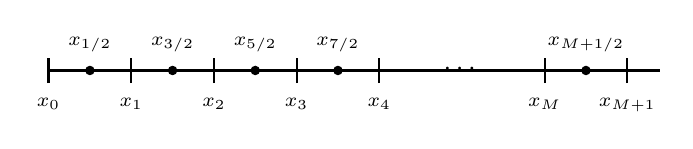
\begin{tikzpicture}[x=1.05cm,y=1cm]
  \draw[thick] (0,0) -- (7.4,0);
  \foreach \i/\lab in {0/{x_{0}},1/{x_{1}},2/{x_{2}},3/{x_{3}},4/{x_{4}}}{
     \draw[thick] (\i,-0.16) -- (\i,0.16);
     \node[below=2pt] at (\i,-0.16) {\scriptsize$\lab$};}
  \foreach \i/\lab in {6/{x_{M}},7/{x_{M+1}}}{
     \draw[thick] (\i,-0.16) -- (\i,0.16);
     \node[below=2pt] at (\i,-0.16) {\scriptsize$\lab$};}
  \foreach \i/\lab in {0.5/{x_{1/2}},1.5/{x_{3/2}},2.5/{x_{5/2}},3.5/{x_{7/2}},
                       6.5/{x_{M+1/2}}}{
     \filldraw (\i,0) circle (1.5pt);
     \node[above=3pt] at (\i,0) {\scriptsize$\lab$};}
  \node at (5,0.02) {$\cdots$};
\end{tikzpicture}
\end{center}

\noindent
The half-integer nodes need not be the midpoints, but we take them to be.

\begin{intuition}[what the extra node buys]
CG(1) fitted a straight line on each element, so two endpoint values pinned it
down. A parabola has three coefficients, so it needs a third condition, and the
cheapest place to put it is inside the element. The submesh node
$x_{j-1/2}$ is not a new mesh point --- the elements are unchanged --- it is
just a third \emph{degree of freedom} carried by the same element.
\end{intuition}

\begin{mechanics}
This is the three-node bar element. CG(1) is the 2-node linear bar with constant
strain; CG(2) is the 3-node quadratic bar whose strain varies linearly along the
element. The midside node is exactly the midside node of a Q8 or T6 element.
\end{mechanics}

% ------------------------------------------------------------------
\subsubsection*{The basis}

For a given element there are $3$ Lagrange polynomials:

\begin{center}
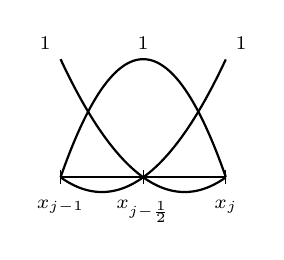
\begin{tikzpicture}[x=2.1cm,y=1.5cm]
  \draw[thick] (0,0) -- (1,0);
  \foreach \i/\lab in {0/{x_{j-1}},0.5/{x_{j-\frac12}},1/{x_{j}}}{
     \draw (\i,-0.06) -- (\i,0.06);
     \node[below=2pt] at (\i,-0.06) {\scriptsize$\lab$};}
  % L_left = 2t^2-3t+1 ; L_mid = 4t(1-t) ; L_right = 2t^2-t
  \draw[thick,domain=0:1,samples=60,smooth]
        plot (\x,{2*\x*\x-3*\x+1});
  \draw[thick,domain=0:1,samples=60,smooth]
        plot (\x,{4*\x*(1-\x)});
  \draw[thick,domain=0:1,samples=60,smooth]
        plot (\x,{2*\x*\x-\x});
  \node[above left]  at (0,1)   {\scriptsize$1$};
  \node[above]       at (0.5,1) {\scriptsize$1$};
  \node[above right] at (1,1)   {\scriptsize$1$};
\end{tikzpicture}
\end{center}

\noindent
As \emph{basis functions} over the whole mesh there are two shapes: the one
sitting at an integer node, which spans two elements, and the bubble sitting at
a half-integer node, which lives inside one element.

\begin{center}
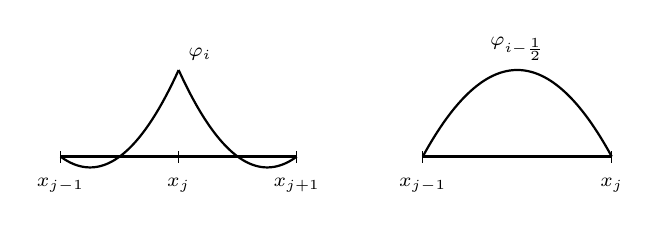
\begin{tikzpicture}[x=1.5cm,y=1.1cm]
  \begin{scope}
  \draw[thick] (0,0) -- (2,0);
  \foreach \i/\lab in {0/{x_{j-1}},1/{x_{j}},2/{x_{j+1}}}{
     \draw (\i,-0.07) -- (\i,0.07);
     \node[below=2pt] at (\i,-0.07) {\scriptsize$\lab$};}
  \draw[thick,domain=0:1,samples=50,smooth] plot (\x,{2*\x*\x-\x});
  \draw[thick,domain=1:2,samples=50,smooth]
        plot (\x,{2*(\x-1)*(\x-1)-3*(\x-1)+1});
  \node[above right] at (1,1) {\scriptsize$\phih_{i}$};
  \end{scope}
  \begin{scope}[xshift=4.6cm]
  \draw[thick] (0,0) -- (1.6,0);
  \foreach \i/\lab in {0/{x_{j-1}},1.6/{x_{j}}}{
     \draw (\i,-0.07) -- (\i,0.07);
     \node[below=2pt] at (\i,-0.07) {\scriptsize$\lab$};}
  \draw[thick,domain=0:1.6,samples=60,smooth]
        plot (\x,{4*(\x/1.6)*(1-\x/1.6)});
  \node[above] at (0.8,1) {\scriptsize$\phih_{i-\frac12}$};
  \end{scope}
\end{tikzpicture}
\end{center}

Explicitly,
\begin{equation}\label{eq:l10phii}
  \phih_{i}(x)=
  \begin{cases}
    \dfrac{2\bigl(x-x_{i+\frac12}\bigr)\bigl(x-x_{i+1}\bigr)}
          {\bigl(x_{i+1}-x_{i}\bigr)^{2}}, & x_{i}\le x\le x_{i+1},\\[2.2ex]
    \dfrac{2\bigl(x-x_{i-\frac12}\bigr)\bigl(x-x_{i-1}\bigr)}
          {\bigl(x_{i}-x_{i-1}\bigr)^{2}}, & x_{i-1}\le x\le x_{i},\\[2.2ex]
    0, & \text{otherwise,}
  \end{cases}
\end{equation}
\begin{equation}\label{eq:l10phihalf}
  \phih_{i-\frac12}(x)=
  \begin{cases}
    \dfrac{4\bigl(x_{i}-x\bigr)\bigl(x-x_{i-1}\bigr)}
          {\bigl(x_{i}-x_{i-1}\bigr)^{2}}, & x_{i-1}\le x\le x_{i},\\[2.2ex]
    0, & \text{otherwise.}
  \end{cases}
\end{equation}
Therefore
\begin{equation}\label{eq:l10span}
  \Vh=\operatorname{span}\bigl\{\phih_{\frac12},\phih_{1},\phih_{\frac32},
      \phih_{2},\dots,\phih_{M},\phih_{M+\frac12}\bigr\},
\end{equation}
so if $U\in\Vh$ then
\begin{equation}\label{eq:l10U}
  U(x)=\sum_{j=1}^{2M+1}\xi_{j}\,\phih_{j/2}(x).
\end{equation}

\medskip\noindent
\textbf{Note.} For any function $v\in\Vsp$,
\begin{equation}\label{eq:l10interp}
  \Pi_h v=\sum_{k=1}^{2M+1}v\bigl(x_{k/2}\bigr)\phih_{k/2}(x),
\end{equation}
and the test functions are $v=\phih_{i/2}(x)$ for $i=1,2,\dots,2M+1$.

% ------------------------------------------------------------------
\subsubsection*{CG(2) variational problem}

\begin{equation}\label{eq:l10cg2var}
  \sum_{j=1}^{2M+1}\xi_{j}\int_0^1 a(x)\,\phih'_{i/2}\phih'_{j/2}\dx
  =\int_0^1 f\,\phih_{i/2}\dx .
\end{equation}
This is a $(2M+1)\times(2M+1)$ symmetric positive definite system, \emph{but not
tridiagonal}.

\begin{pitfall}[the bandwidth changes, not just the size]
Going from CG(1) to CG(2) is not simply ``more unknowns.'' A basis function at
an integer node now overlaps the bubbles on \emph{both} neighbouring elements
and the integer node two slots away, so the matrix picks up a second
off-diagonal: it becomes pentadiagonal. Higher order buys accuracy per node and
pays for it in bandwidth --- the same trade a higher-order element makes in a
commercial solver.
\end{pitfall}

% ------------------------------------------------------------------
\subsubsection*{Example: $a\equiv1$ and $h_{j}=h$ for all $j$}

\noindent\textbf{Stiffness matrix.}

\medskip
\textcircled{\scriptsize1}\; $i=1,3,\dots,2M+1$ (the half-integer nodes):
\begin{align}
  A_{ii}&=\int_{x_{\frac{i}{2}-\frac12}}^{x_{\frac{i}{2}+\frac12}}
          \bigl(\phih'_{i/2}\bigr)^{2}\dx=\frac{16}{3h},
          \label{eq:l10Aodd}\\[0.4ex]
  A_{(i-1,i)}=A_{(i,i-1)}&=\int_{x_{\frac{i-1}{2}}}^{x_{\frac{i+1}{2}}}
          \phih'_{i/2}\,\phih'_{\frac{i-1}{2}}\dx=-\frac{8}{3h}.
          \label{eq:l10Aoddoff}
\end{align}

\textcircled{\scriptsize2}\; $i=2,4,6,\dots,2M$ (the integer nodes):
\begin{align}
  A_{ii}&=\int_{x_{\frac{i-1}{2}}}^{x_{\frac{i+1}{2}}}
          \bigl[\phih'_{i/2}\bigr]^{2}\dx=\frac{14}{3h},
          \label{eq:l10Aeven}\\[0.4ex]
  A_{(i,i-1)}=A_{(i-1,i)}&=\int_{x_{\frac{i-1}{2}}}^{x_{\frac{i}{2}}}
          \phih'_{i/2}\,\phih'_{\frac{i}{2}-\frac12}\dx=-\frac{8}{3h},
          \label{eq:l10Aevenoff1}\\[0.4ex]
  A_{(i,i-2)}=A_{(i-2,i)}&=\int_{x_{\frac{i-1}{2}}}^{x_{i/2}}
          \phih'_{i/2}\,\phih'_{\frac{i}{2}-1}\dx=\frac{1}{3h}.
          \label{eq:l10Aevenoff2}
\end{align}

\medskip\noindent\textbf{RHS vector.} Replace $f$ by its interpolant,
\begin{equation}\label{eq:l10fint}
  f\approx\widetilde{\Pi}_h f=\sum_{j=0}^{2M+2}f\bigl(x_{j/2}\bigr)\phih_{j/2}(x).
\end{equation}

\textcircled{\scriptsize1}\; $i=1,3,\dots,2M+1$:
\begin{equation}\label{eq:l10fodd}
  f_{i}=\sum_{j=1}^{2M+1}f\bigl(x_{j/2}\bigr)
        \int_{x_{\frac{i-1}{2}}}^{x_{\frac{i+1}{2}}}\phih_{j/2}\,\phih_{i/2}\dx
      =\frac{h}{15}\Bigl[f\bigl(x_{\frac{i-1}{2}}\bigr)
        +8f\bigl(x_{i/2}\bigr)+f\bigl(x_{\frac{i+1}{2}}\bigr)\Bigr].
\end{equation}

\textcircled{\scriptsize2}\; $i=2,4,\dots,2M$:
\begin{equation}\label{eq:l10feven}
  f_{i}=\frac{h}{30}\Bigl[-f\bigl(x_{\frac{i-2}{2}}\bigr)
        +2f\bigl(x_{\frac{i-1}{2}}\bigr)+8f\bigl(x_{i/2}\bigr)
        +2f\bigl(x_{\frac{i+1}{2}}\bigr)-f\bigl(x_{\frac{i+2}{2}}\bigr)\Bigr].
\end{equation}

\medskip\noindent
Therefore
\begin{equation}\label{eq:l10Amat}
  \bm{A}=\frac{1}{3h}
  \begin{bmatrix}
    16 & -8 &    &    &    &    &   \\
    -8 & 14 & -8 &  1 &    &    &   \\
       & -8 & 16 & -8 &    &    &   \\
       &  1 & -8 & 14 & -8 &  1 &   \\
       &    &    & \ddots & \ddots & \ddots & \\
       &    &    &  1 & -8 & 14 & -8\\
       &    &    &    &    & -8 & 16
  \end{bmatrix},
  \qquad \bm{A}\bm{x}=\bm{b}.
\end{equation}

\medskip\noindent
\textbf{Note (energy norm error).} Galerkin orthogonality gives
$\norm{u-U}_{E}\le\norm{u-v}_{E}$ for all $v\in\Vh$; taking $v=\Pi_h u$,
\begin{equation}\label{eq:l10eng}
  \boxed{\;\norm{u-U}_{E}\le c\,\norm{h^{2}u'''}\;}
\end{equation}

\noindent
\textbf{Note ($L^{2}$ error).}
\begin{equation}\label{eq:l10l2}
  \boxed{\;\norm{u-U}\le c\,\norm{h^{3}u'''}\;}
\end{equation}

\begin{intuition}[what the exponents say]
CG(1) gave $O(h)$ in energy and $O(h^{2})$ in $L^{2}$; CG(2) gives $O(h^{2})$
and $O(h^{3})$. Each extra polynomial degree buys one extra power of $h$ in both
norms, and the $L^{2}$ rate stays one power ahead of the energy rate --- the
duality argument of Lecture 8 is what produces that extra power, and it does not
care what degree the elements are.
\end{intuition}

% ##################################################################
\subsection*{Beam equation}

\begin{equation}\label{eq:l11beam}
  \left\{
  \begin{aligned}
    u^{(iv)}&=f &&\text{on }0<x<1,\\
    u(0)=u'(0)&=u(1)=u'(1)=0 .
  \end{aligned}\right.
\end{equation}

% ------------------------------------------------------------------
\subsubsection*{Variational problem}

Multiply by $v$ and integrate by parts twice:
\begin{align}
  \int_0^1 v\,u^{(iv)}\dx&=\int_0^1 f v\dx ,\label{eq:l11ibp0}\\
  -\int_0^1 v'u'''\dx+\underbrace{\bigl[v\,u'''\bigr]_0^1}_{=\,0}
     &=\int_0^1 f v\dx
     &&\text{(let } v(0)=v(1)=0),\label{eq:l11ibp1}\\
  \int_0^1 v''u''\dx-\underbrace{\bigl[v'u''\bigr]_0^1}_{=\,0}
     &=\int_0^1 f v\dx
     &&\text{(let } v'(0)=v'(1)=0),\label{eq:l11ibp2}
\end{align}
so
\begin{equation}\label{eq:l11weak}
  \int_0^1 u''v''\dx=\int_0^1 f v\dx .
\end{equation}
The space is
\begin{equation}\label{eq:l11V}
  \Vsp=\Bigl\{v:\ \int_0^1\bigl[v^{2}+(v')^{2}+(v'')^{2}\bigr]\dx<\infty,\ \
  v(0)=v(1)=v'(0)=v'(1)=0\Bigr\},
\end{equation}
and functions in $\Vsp$ are $C^{1}[0,1]$.

\medskip
\noindent\fbox{\parbox{0.93\linewidth}{%
\textbf{(Variational problem)} Find $u\in\Vsp$ such that
$\displaystyle\int_0^1 u''v''\dx=\int_0^1 f v\dx$ for all $v\in\Vsp$.}}

\begin{intuition}[why the space jumps from $H^{1}$ to $H^{2}$]
The bar equation lost one derivative to the test function and kept one, so
$\int(v')^{2}<\infty$ was enough. The beam equation has four derivatives to
share, two each, so now $\int(v'')^{2}<\infty$ is required. That extra
requirement is what forces $C^{1}$: a function with a corner has a jump in $v'$,
hence a delta in $v''$, hence $\int(v'')^{2}=\infty$. Kinks were legal for the
bar; they are illegal for the beam.
\end{intuition}

\begin{mechanics}
$\tfrac12\int(u'')^{2}$ is the bending strain energy $\tfrac12\int EI\,\kappa^{2}$
with $EI\equiv1$, since $u''$ is the curvature. Requiring finite bending energy
is requiring $u\in H^{2}$. And $C^{1}$ continuity is just the physical statement
that a beam does not develop a kink under a distributed load --- deflection
\emph{and} slope must match across an element boundary.
\end{mechanics}

% ------------------------------------------------------------------
\subsubsection*{Energy minimization}

Define
\begin{equation}\label{eq:l11F}
  F(w)=\frac12\int_0^1(w'')^{2}\dx-\int_0^1 f w\dx .
\end{equation}

\noindent\fbox{\parbox{0.93\linewidth}{%
\textbf{(Minimization problem)} Find $u\in\Vsp$ such that
$F(u)\le F(w)$ for all $w\in\Vsp$.}}

\medskip\noindent
\textbf{Claim.} (Var.\ Prob.)\;$\Longleftrightarrow$\;(Min.\ Prob.)

\medskip\noindent
($\Longrightarrow$) Assume $u\in\Vsp$ satisfies the variational problem. Let
$w=u+v\in\Vsp$. Then
\begin{align}
  F(w)=F(u+v)&=\underbrace{\frac12\int_0^1(u'')^{2}\dx-\int_0^1 fu\dx}_{=\,F(u)}
    \;+\;\frac12\int_0^1(v'')^{2}\dx
    \;+\;\underbrace{\int_0^1 u''v''\dx-\int_0^1 f v\dx}_{=\,0\ \text{by \eqref{eq:l11weak}}},
    \label{eq:l11expand}
\end{align}
so
\begin{equation}\label{eq:l11FwFu}
  F(w)=F(u)+\frac12\int_0^1(v'')^{2}\dx\;\ge\;F(u).
\end{equation}

\medskip\noindent
\textbf{Note.} $F(w)=F(u)\ \Rightarrow\ v''\equiv0\ \Rightarrow\ v\equiv0$
(due to the BCs) $\Rightarrow\ u\equiv w$.

\begin{intuition}[why $v''\equiv 0$ forces $v\equiv 0$ here]
$v''\equiv0$ only says $v$ is a straight line, $v=\alpha+\beta x$. It is the
four boundary conditions in \eqref{eq:l11V} that kill it: $v(0)=v'(0)=0$ already
force $\alpha=\beta=0$. For the bar, the same step used $v'\equiv0$ plus the two
Dirichlet conditions. Same mechanism, one derivative higher.
\end{intuition}

% ------------------------------------------------------------------
\subsection*{CG(3) method}

We need $\Vh\subseteq\Vsp$. On each element $[x_{j-1},x_{j}]$ we need a
polynomial that matches \emph{value and derivative} to its neighbours at
$x_{j-1}$ and $x_{j}$ --- that is $4$ conditions, so we need a cubic
($4$ coefficients):
\begin{equation}\label{eq:l11Vh}
  \Vh=\bigl\{v\in\Vsp:\ v|_{[x_{j-1},x_{j}]}
      =a_{j}+b_{j}x+c_{j}x^{2}+d_{j}x^{3}\bigr\}.
\end{equation}

\medskip\noindent
\textbf{Key:} find a basis for $\Vh$. Two basis functions are attached to each
node --- one controlling the value, one controlling the slope:

\begin{center}
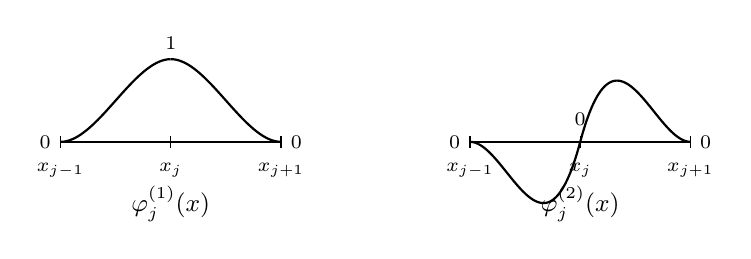
\begin{tikzpicture}[x=1.4cm,y=1.05cm]
  \begin{scope}
  \draw[thick] (0,0) -- (2,0);
  \foreach \i/\lab in {0/{x_{j-1}},1/{x_{j}},2/{x_{j+1}}}{
     \draw (\i,-0.07) -- (\i,0.07);
     \node[below=2pt] at (\i,-0.07) {\scriptsize$\lab$};}
  \draw[thick,domain=0:1,samples=60,smooth] plot (\x,{3*\x*\x-2*\x*\x*\x});
  \draw[thick,domain=1:2,samples=60,smooth]
        plot (\x,{3*(2-\x)*(2-\x)-2*(2-\x)*(2-\x)*(2-\x)});
  \node[above] at (1,1) {\scriptsize$1$};
  \node[left]  at (0,0) {\scriptsize$0$};
  \node[right] at (2,0) {\scriptsize$0$};
  \node at (1,-0.75) {\small$\phih_{j}^{(1)}(x)$};
  \end{scope}
  \begin{scope}[xshift=5.2cm]
  \draw[thick] (0,0) -- (2,0);
  \foreach \i/\lab in {0/{x_{j-1}},1/{x_{j}},2/{x_{j+1}}}{
     \draw (\i,-0.07) -- (\i,0.07);
     \node[below=2pt] at (\i,-0.07) {\scriptsize$\lab$};}
  % left: t^2(t-1) scaled ; right: u^2(1+u) with u=x-2
  \draw[thick,domain=0:1,samples=60,smooth]
        plot (\x,{5*(\x*\x*(\x-1))});
  \draw[thick,domain=1:2,samples=60,smooth]
        plot (\x,{5*((\x-2)*(\x-2)*(1+\x-2))});
  \node[left]  at (0,0) {\scriptsize$0$};
  \node[above] at (1,0.08) {\scriptsize$0$};
  \node[right] at (2,0) {\scriptsize$0$};
  \node at (1,-0.75) {\small$\phih_{j}^{(2)}(x)$};
  \end{scope}
\end{tikzpicture}
\end{center}

\noindent
They are fixed by the nodal table
\begin{center}\small
\renewcommand{\arraystretch}{1.35}
\begin{tabular}{@{}l|ccc@{}}
\toprule
 & $x_{j-1}$ & $x_{j}$ & $x_{j+1}$\\
\midrule
$\phih_{j}^{(1)}$      & $0$ & $1$ & $0$\\
$\bigl(\phih_{j}^{(1)}\bigr)'$ & $0$ & $0$ & $0$\\
$\phih_{j}^{(2)}$      & $0$ & $0$ & $0$\\
$\bigl(\phih_{j}^{(2)}\bigr)'$ & $0$ & $1$ & $0$\\
\bottomrule
\end{tabular}
\end{center}

\noindent
which gives
\begin{equation}\label{eq:l11phi1}
  \phih_{j}^{(1)}=
  \begin{cases}
    3\left(\dfrac{x-x_{j-1}}{x_{j}-x_{j-1}}\right)^{2}
      -2\left(\dfrac{x-x_{j-1}}{x_{j}-x_{j-1}}\right)^{3},
      & x_{j-1}\le x\le x_{j},\\[3ex]
    3\left(\dfrac{x-x_{j+1}}{x_{j}-x_{j+1}}\right)^{2}
      -2\left(\dfrac{x-x_{j+1}}{x_{j}-x_{j+1}}\right)^{3},
      & x_{j}\le x\le x_{j+1},\\[3ex]
    0, & \text{otherwise,}
  \end{cases}
\end{equation}
\begin{equation}\label{eq:l11phi2}
  \phih_{j}^{(2)}=
  \begin{cases}
    -\dfrac{1}{h_{j}}\bigl(x-x_{j-1}\bigr)^{2}
      +\dfrac{1}{h_{j}^{2}}\bigl(x-x_{j-1}\bigr)^{3},
      & x_{j-1}\le x\le x_{j},\\[3ex]
    \dfrac{1}{h_{j+1}}\bigl(x-x_{j+1}\bigr)^{2}
      +\dfrac{1}{h_{j+1}^{2}}\bigl(x-x_{j+1}\bigr)^{3},
      & x_{j}\le x\le x_{j+1},\\[3ex]
    0, & \text{otherwise.}
  \end{cases}
\end{equation}

\medskip\noindent\fbox{\parbox{0.93\linewidth}{%
\textbf{CG(3) FEM:} Find $U\in\Vh$ such that
$\displaystyle\int_0^1 U''v''\dx=\int_0^1 f v\dx$ for all $v\in\Vh$.}}

\begin{mechanics}
This is the Hermite beam element, exactly as it appears in a structural code.
$\phih_{j}^{(1)}$ and $\phih_{j}^{(2)}$ are the cubic Hermite shape functions
$N_{1},N_{2},N_{3},N_{4}$; node $j$ carries two degrees of freedom, a deflection
and a rotation. The table above is the statement $N_{i}(\text{dof}_{k})=
\delta_{ik}$ --- each shape function switches on one dof and leaves the other
three at zero. The $C^{1}$ requirement is why a beam element has a rotational
dof at all, while a bar element does not.
\end{mechanics}

\todoq{In the nodal table for the Hermite basis, the entry for
$\bigl(\phih_{j}^{(1)}\bigr)'$ at $x_{j}$ is written in a way that reads as a
$6$ in the scan. It has to be $0$ --- \eqref{eq:l11phi1} has a flat top at
$x_{j}$ --- and I have transcribed it as $0$. Worth a glance at the original.}

\todoq{Page~4 of the scan writes the two CG(2) error notes with $u'''$ on both
right-hand sides, $\norm{u-U}_{E}\le c\norm{h^{2}u'''}$ and
$\norm{u-U}\le c\norm{h^{3}u'''}$. Check whether the second was meant to carry
$u'''$ or $u^{(4)}$.}

\lecture{CG(3) assembly: the Hermite stiffness matrix}{Lecture 12 --- Wednesday, September 23, 2026}{Math 6660 --- \texttt{12th.pdf}}

\noindent{\small\itshape Lecture 12 re-states the beam problem from
Lecture 11 and then carries the CG(3) discretisation all the way to the
assembled linear system. Pages 7--9 of \texttt{missing.pdf} cover the same
material; the two sources agree throughout, and the transcription below follows
my own notes.}

\begin{roadmap}[Lecture 12]
\roadq{What does the beam stiffness matrix actually look like once assembled?}
\begin{roadlist}
\item Two kinds of unknown per node (a value, a slope) means every matrix entry
  is one of four pairings. The matrix splits into blocks: $\bm{A}$
  deflection--deflection, $\bm{B}$ rotation--rotation, $\bm{C}$ the coupling.
\item $\bm{C}$ is \emph{anti}-symmetric --- and the assembled $\bm{S}$ is still
  symmetric. Worth understanding rather than memorising.
\item The load side now needs \textbf{two} vectors: a distributed load lumps
  into nodal forces \emph{and} nodal moments.
\item The numbers that come out --- $12/h^{3}$, $6/h^{2}$, $4/h$, $2/h$ --- are
  the textbook Euler--Bernoulli element matrix with $EI=1$.
\end{roadlist}
\payoff{Recognising the beam element you already know, written in the
mathematics department's notation.}
\end{roadmap}

% ==================================================================
\subsection*{Recap: the beam problem and its CG(3) space}

\begin{equation}\label{eq:l12beam}
  \left\{
  \begin{aligned}
    u^{(iv)}&=f &&\text{in }(0,1),\\
    u(0)=u(1)&=u'(0)=u'(1)=0 ,
  \end{aligned}\right.
\end{equation}
\begin{equation}\label{eq:l12V}
  \Vsp=\Bigl\{v:\ \int_0^1\bigl[v^{2}+(v')^{2}+(v'')^{2}\bigr]\dx<\infty,\ \
  v(0)=v(1)=v'(0)=v'(1)=0\Bigr\}.
\end{equation}
Functions in $\Vsp$ are $C^{1}$. Find $u\in\Vsp$ such that
\begin{equation}\label{eq:l12weak}
  \int_0^1 u''v''\dx=\int_0^1 f v\dx\qquad\forall\,v\in\Vsp .
\end{equation}

\medskip\noindent
\textbf{FEM:} $\Vh\subset\Vsp$, spanned by the two Hermite shapes per node ---
$\phih_{j}^{(1)}$, which carries the nodal value, and $\phih_{j}^{(2)}$, which
carries the nodal slope (Lecture 11, \eqref{eq:l11phi1}--\eqref{eq:l11phi2}):
\begin{equation}\label{eq:l12span}
  \Vh=\operatorname{span}\bigl\{\phih_{1}^{(1)},\dots,\phih_{M}^{(1)},\
      \phih_{1}^{(2)},\dots,\phih_{M}^{(2)}\bigr\},\qquad\dim\Vh=2M .
\end{equation}
\textbf{Trial functions:}
\begin{equation}\label{eq:l12trial}
  U=\sum_{j=1}^{M}\xi_{j}\,\phih_{j}^{(1)}(x)
    +\sum_{j=1}^{M}\eta_{j}\,\phih_{j}^{(2)}(x).
\end{equation}
\textbf{Test functions:} $v=\phih_{1}^{(1)},\dots,\phih_{M}^{(1)},
\phih_{1}^{(2)},\dots,\phih_{M}^{(2)}$.

% ==================================================================
\subsection*{The interpolant and its errors}

If $u\in\Vsp$, then
\begin{equation}\label{eq:l12PI}
  \Pi_h u=\sum_{j=1}^{M}u(x_{j})\,\phih_{j}^{(1)}(x)
          +\sum_{j=1}^{M}u'(x_{j})\,\phih_{j}^{(2)}(x),
  \qquad\text{where }\Pi_h u\in\Vh .
\end{equation}

\medskip\noindent
\textbf{Interpolation errors:}
\begin{align}
  \norm{u-\Pi_h u}_{\Ltwo[0,1]}     &\le c_{1}\norm{h^{4}u^{(4)}}_{\Ltwo[0,1]},
     \label{eq:l12int0}\\
  \norm{(u-\Pi_h u)'}_{\Ltwo[0,1]}  &\le c_{2}\norm{h^{3}u^{(4)}}_{\Ltwo[0,1]},
     \label{eq:l12int1}\\
  \norm{(u-\Pi_h u)''}_{\Ltwo[0,1]} &\le c_{3}\norm{h^{2}u^{(4)}}_{\Ltwo[0,1]}.
     \label{eq:l12int2}
\end{align}

\begin{intuition}[why $u^{(4)}$, and why the exponents step down]
The Hermite interpolant matches value and slope at both ends of every element,
so it reproduces \emph{every cubic exactly}. The first thing it cannot
reproduce is the fourth derivative --- which is why $u^{(4)}$, and nothing
lower, sits on every right-hand side. Each derivative you take of the error
costs one power of $h$: $h^{4}$ for the function, $h^{3}$ for the slope,
$h^{2}$ for the curvature. Since the energy norm for the beam measures $v''$,
\eqref{eq:l12int2} is the one that controls the FEM error, giving $O(h^{2})$.
\end{intuition}

% ==================================================================
\subsection*{Example: uniform mesh, $h_{j}=h$ for all $j$}

With
\begin{equation}\label{eq:l12fem}
  \int_0^1 U''v''\dx=\int_0^1 f v\dx,
  \qquad v=\phih_{1}^{(1)},\dots,\phih_{M}^{(1)},
            \phih_{1}^{(2)},\dots,\phih_{M}^{(2)} ,
\end{equation}
the stiffness matrix comes out of four families of integrals. Testing against
$\phih_{k}^{(1)}$, $k=1,2,\dots,M$:
\begin{equation}\label{eq:l12rowa}
  \int_0^1 U''v''\dx
  =\sum_{j=1}^{M}\xi_{j}\int_0^1\bigl(\phih_{j}^{(1)}\bigr)''
     \bigl(\phih_{k}^{(1)}\bigr)''\dx
  +\sum_{j=1}^{M}\eta_{j}\int_0^1\bigl(\phih_{j}^{(2)}\bigr)''
     \bigl(\phih_{k}^{(1)}\bigr)''\dx ,
\end{equation}
and then again, testing against $\phih_{k}^{(2)}$, $k=1,2,\dots,M$:
\begin{equation}\label{eq:l12rowb}
  \sum_{j=1}^{M}\xi_{j}\int_0^1\bigl(\phih_{j}^{(1)}\bigr)''
     \bigl(\phih_{k}^{(2)}\bigr)''\dx
  +\sum_{j=1}^{M}\eta_{j}\int_0^1\bigl(\phih_{j}^{(2)}\bigr)''
     \bigl(\phih_{k}^{(2)}\bigr)''\dx .
\end{equation}
That is a block matrix
\begin{equation}\label{eq:l12block}
  \left[\begin{array}{c|c}
    \bm{A} & \bm{C}\\\hline
    -\bm{C} & \bm{B}
  \end{array}\right]\in\R^{2M\times2M},
  \qquad\text{here }\bm{A},\bm{B},\bm{C}\in\R^{M\times M}.
\end{equation}

\begin{intuition}[where the four blocks come from]
There are two kinds of unknown ($\xi$, a value; $\eta$, a slope) and two kinds
of test function, so every entry of the matrix is one of four pairings:
value--value, value--slope, slope--value, slope--slope. $\bm{A}$ is the first,
$\bm{B}$ the last, $\bm{C}$ the cross terms. Nothing about the physics changed
--- it is still $\int u''v''$ --- only the bookkeeping, because each node now
carries two numbers.
\end{intuition}

% ------------------------------------------------------------------
\subsubsection*{The three blocks}

\medskip\noindent
Now,
\begin{equation}\label{eq:l12Ajk}
  A_{jk}=\int_0^1\bigl(\phih_{j}^{(1)}\bigr)''\bigl(\phih_{k}^{(1)}\bigr)''\dx,
  \qquad
  \bm{A}=\frac{12}{h^{3}}
  \begin{bmatrix}
    2 & -1 &        &    \\
   -1 &  2 & \ddots &    \\
      & \ddots & \ddots & -1\\
      &    & -1 & 2
  \end{bmatrix},
\end{equation}
which is $M\times M$, tridiagonal, symmetric.

\begin{equation}\label{eq:l12Bjk}
  B_{jk}=\int_0^1\bigl(\phih_{j}^{(2)}\bigr)''\bigl(\phih_{k}^{(2)}\bigr)''\dx,
  \qquad
  \bm{B}=\frac{2}{h}
  \begin{bmatrix}
    4 & 1 &        &   \\
    1 & 4 & \ddots &   \\
      & \ddots & \ddots & 1\\
      &   & 1 & 4
  \end{bmatrix},
\end{equation}
which is $M\times M$, tridiagonal, symmetric.

\begin{equation}\label{eq:l12Cjk}
  C_{jk}=\int_0^1\bigl(\phih_{j}^{(1)}\bigr)''\bigl(\phih_{k}^{(2)}\bigr)''\dx,
  \qquad
  \bm{C}=\frac{6}{h^{2}}
  \begin{bmatrix}
    0 & 1 &        &   \\
   -1 & 0 & \ddots &   \\
      & \ddots & \ddots & 1\\
      &   & -1 & 0
  \end{bmatrix},
\end{equation}
which is $M\times M$, tridiagonal --- but \emph{not} symmetric. It is
anti-symmetric:
\begin{equation}\label{eq:l12anti}
  \bm{C}^{T}=-\bm{C}.
\end{equation}
Therefore
\begin{equation}\label{eq:l12S}
  \bm{S}=\left[\begin{array}{c|c}
    \bm{A} & \bm{C}\\\hline
    \bm{C}^{T} & \bm{B}
  \end{array}\right],
  \qquad \bm{S}^{T}=\bm{S},
\end{equation}
so $\bm{S}$ is $2M\times2M$ and symmetric.

\begin{pitfall}[an anti-symmetric block does not break symmetry]
$\bm{C}^{T}=-\bm{C}$ is exactly what makes $\bm{S}$ symmetric: the lower-left
block \emph{is} $\bm{C}^{T}$, so writing it as $-\bm{C}$ in
\eqref{eq:l12block} is the same statement. The minus sign is a consequence of
the sign convention for the slope degree of freedom, not a loss of symmetry ---
$\int u''v''$ is self-adjoint, so the matrix could not have come out
unsymmetric.
\end{pitfall}

\begin{mechanics}
The $12/h^{3}$, $6/h^{2}$, $4/h$, $2/h$ pattern in
\eqref{eq:l12Ajk}--\eqref{eq:l12Cjk} is the classical Euler--Bernoulli beam
element stiffness matrix with $EI=1$. In a structural code the element matrix
is written once as
$\frac{EI}{L^{3}}\begin{bsmallmatrix}12&6L&-12&6L\\6L&4L^{2}&-6L&2L^{2}\\
-12&-6L&12&-6L\\6L&2L^{2}&-6L&4L^{2}\end{bsmallmatrix}$
and assembled; here the same numbers arrive sorted by \emph{type} of degree of
freedom instead of by node, which is why they appear as three separate blocks.
\end{mechanics}

% ==================================================================
\subsection*{RHS}

Interpolate the load with the same Hermite basis,
\begin{equation}\label{eq:l12fint}
  f\ \longrightarrow\ \widetilde{\Pi}_h f
  =\sum_{j=0}^{M+1}f(x_{j})\,\phih_{j}^{(1)}(x)
   +\sum_{j=0}^{M+1}f'(x_{j})\,\phih_{j}^{(2)}(x),
\end{equation}
\begin{equation}\label{eq:l12fsub}
  \int_0^1 f v\dx\ \longrightarrow\ \int_0^1\bigl(\widetilde{\Pi}_h f\bigr)v\dx .
\end{equation}
Now, for $j=1,2,\dots,M$,
\begin{align}
  f_{j}^{(1)}&=\frac{h}{70}\Bigl[9f(x_{j-1})+52f(x_{j})+9f(x_{j+1})\Bigr]
     +\frac{13h^{2}}{420}\Bigl[f'(x_{j-1})-f'(x_{j+1})\Bigr],
     \label{eq:l12f1}\\[0.6ex]
  f_{j}^{(2)}&=\frac{13h^{2}}{420}\Bigl[f(x_{j+1})-f(x_{j-1})\Bigr]
     -\frac{h^{3}}{420}\Bigl[3f'(x_{j-1})-8f'(x_{j})+3f'(x_{j+1})\Bigr].
     \label{eq:l12f2}
\end{align}

% ==================================================================
\subsection*{The final system}

\begin{equation}\label{eq:l12system}
  \left[\begin{array}{c|c}
    \bm{A} & \bm{C}\\\hline
    -\bm{C} & \bm{B}
  \end{array}\right]
  \left[\begin{array}{c}\bm{\xi}\\\hline\bm{\eta}\end{array}\right]
  =\left[\begin{array}{c}\bm{f}^{(1)}\\\hline\bm{f}^{(2)}\end{array}\right],
\end{equation}
which is $2M\times2M$, symmetric, positive definite. Here $\bm{\eta}$ is the
vector of \emph{derivative values at the nodes}.

\begin{mechanics}
\eqref{eq:l12system} is the assembled beam problem in the form a structural
solver produces it: $\bm{\xi}$ are the nodal deflections, $\bm{\eta}$ the nodal
rotations, $\bm{f}^{(1)}$ the consistent nodal forces and $\bm{f}^{(2)}$ the
consistent nodal moments. The $13h^{2}/420$ and $h^{3}/420$ coefficients in
\eqref{eq:l12f1}--\eqref{eq:l12f2} are the consistent load vector for a
distributed load on a Hermite beam element --- the same numbers a code computes
when you apply a pressure rather than a point load.
\end{mechanics}

\begin{dictionary}[beam FEM]
$\xi_{j}$, the coefficient of $\phih_{j}^{(1)}$ & the nodal deflection $w_{j}$\\
$\eta_{j}$, the coefficient of $\phih_{j}^{(2)}$ & the nodal rotation $\theta_{j}$\\
$\bm{A}$ block & deflection--deflection stiffness\\
$\bm{B}$ block & rotation--rotation stiffness\\
$\bm{C}$ block & the deflection--rotation coupling\\
$\bm{S}$ symmetric positive definite & the structure is stable and the energy is a genuine minimum\\
$\widetilde{\Pi}_h f$ & lumping the distributed load onto nodal forces and moments\\
\end{dictionary}

\todoq{On page~2 the first interpolation error is written
$\norm{u-\Pi_h u}\le c_{1}\norm{h^{4}u^{4}}$ --- the exponent on $u$ should be
the superscript $(4)$, matching the other two lines; transcribed as $u^{(4)}$.
Similarly the second sum in $\Pi_h u$ on that page runs to $n$ rather than $M$.}


\end{document}
